\documentclass{scu-thesis}
\usepackage{amsmath}	% for advanced typesetting of mathematics
\usepackage{graphicx}	% for including graphics
\usepackage[numbers]{natbib}	% for better citation styles
\usepackage{txfonts}	% for using the Times-Roman font
\usepackage{multirow}
\usepackage{multicol}
\usepackage{arydshln}
\usepackage{float}
\setcitestyle{square}
\usepackage{listings}
\usepackage{xcolor}

\definecolor{codegreen}{rgb}{0,0.6,0}
\definecolor{codegray}{rgb}{0.5,0.5,0.5}
\definecolor{codepurple}{rgb}{0.58,0,0.82}
\definecolor{backcolour}{rgb}{0.95,0.95,0.92}

\lstdefinestyle{mystyle}{
    backgroundcolor=\color{backcolour},   
    commentstyle=\color{codegreen},
    keywordstyle=\color{magenta},
    numberstyle=\tiny\color{codegray},
    stringstyle=\color{codepurple},
    basicstyle=\ttfamily\footnotesize,
    breakatwhitespace=false,         
    breaklines=true,                 
    captionpos=b,                    
    keepspaces=true,                 
    numbers=left,                    
    numbersep=5pt,                  
    showspaces=false,                
    showstringspaces=false,
    showtabs=false,                  
    tabsize=2
}

\lstset{style=mystyle}

% These must be set first ... the rest of the thesis commands rely on them.

\author{Madeleine Waldie}
\title{The Journey to Desensitization: A Mobile App for Oral Immunotherapy Patients}
\department{Department of Computer Science and Engineering}
\degree{Bachelor of Science in Computer Science and Engineering}

% Only bachelor's theses should have multiple authors and/or be from
% multiple departments.  Signatures required:
%
% Bachelor's theses: advisor(s), department chair(s)
% Master's theses: advisor, reader, department chair
% Doctoral theses: doctoral committee (including advisor), department chair

\begin{document}
\frontmatter
\signature{Thesis Advisor}
% \signature{Thesis Advisor}
\signature{Department Chair}
% \signature{Department Chair}

\maketitle
\begin{abstract}
Millions of individuals in the United States confront the daily challenges of food allergies, with the threat of potentially life-threatening reactions ever-present. Oral Immunotherapy (OIT) emerges as a beacon of hope in this landscape, gradually desensitizing patients to their allergens. This groundbreaking treatment, contrasting avoidance strategies, promises a life with fewer restrictions. However, it is a journey fraught with complexities, requiring rigorous adherence to protocols, emotional fortitude, and frequent medical supervision for patients. This thesis centers on the creation of an iPhone application tailored to OIT patients, leveraging Apple's privacy and security features. The app integrates seamlessly with the Apple Health app, providing a platform for dose tracking, symptom logging, and the visualization of long-term trends. As a comprehensive resource, it educates users about anaphylaxis and OIT. This project seeks to address the unmet needs of OIT patients, offering vital support, guidance, and resources, ultimately enhancing the quality of life for those grappling with food allergies.
\end{abstract}


\tableofcontents
\listoftables
\listoffigures

\mainmatter
\chapter{Introduction}

\section{Background}

Every day, approximately 32 million Americans grapple with the challenges of food allergies \cite{FARE}. A staggering 10 percent of the population finds itself on the precipice of a potentially life-threatening reaction with every meal. 

Living with food allergies is a relentless battle – a constant state of vigilance. The mere act of eating transforms into a high-stakes game of Russian roulette, where the wrong choice can lead to dire consequences. Exclusion from social activities, bullying, and the looming specter of emergency room visits become haunting hallmarks of life for those afflicted \cite{Brown}. Having lived with life-threatening, airborne food allergies my entire life, I know firsthand what this is like. In the first six months of my junior year of high school, I had over thirty-two allergic reactions, received seven epinephrine injections, was evacuated from school by ambulance four times, and was hospitalized once. The physical and emotional toll of living like this is immeasurable.

However, there is a glimmer of hope on the horizon – oral immunotherapy. Oral immunotherapy (OIT) is a medical treatment that gradually exposes a person to increasing amounts of an allergen to desensitize them to it. The goal of OIT is to help people with food allergies develop a tolerance to an allergen so that they can safely consume small amounts of it without experiencing an allergic reaction \cite{AAAAI}. This groundbreaking approach represents a paradigm shift in the treatment of food allergies. Unlike the decades-old strategy of avoidance \cite{ACAAI}, oral immunotherapy offers the prospect of desensitizing patients to their allergens. By reaching a maintenance dose, a new level of protection allows them to be near, touch, or even consume foods they were previously forced to shun. This revolutionary approach has shown remarkable promise in clinical trials, raising the possibility of a life with fewer dietary restrictions and reduced fear of accidental allergen exposure.

Despite its immense potential, oral immunotherapy is not without its complexities and uncertainties – especially for the patient. It requires rigorous adherence to protocols, frequent medical supervision, and the emotional fortitude to face one's allergens head-on – not to mention, patients frequently experience side effects when updosing (i.e., increasing the intake of their allergen), such as itchiness or vomiting, and risk more severe complications, like anaphylaxis.

As with any medical treatment, patients need to log their doses and symptoms to keep track of their progress. But, for many, this is a difficult, impractical task. The magnitude of this challenge is evident in my three-inch binder filled with over 1,600 handwritten logs from my five-year OIT journey. And this binder will only grow, as I continue to take my maintenance dose of OIT for the rest of my life.

The lack of accessible tools to support patients throughout this journey is glaring, and it is within this context that the need for an innovative solution emerges. The overarching problem addressed by this thesis lies in the unmet needs of oral immunotherapy patients. These individuals require comprehensive support, guidance, and resources to navigate the intricate path toward desensitization safely and effectively. 

\section{Project Goal}

This project primarily focuses on the design and development of an iPhone application for OIT patients. By opting for the iOS platform, I aim to leverage Apple's robust privacy and security features, ensuring the safe storage of sensitive information. A key feature of the app will be its integration with the Apple Health app, allowing users to seamlessly view their oral immunotherapy data with other health metrics such as exercise and heart rate, all of which can significantly influence treatment outcomes. Integration with the Apple Health app will allow patients to easily, and securely, share their OIT information with their doctors.

Not only will the app facilitate daily dose tracking and symptom logging, but also it will provide the visualization of long-term trends, providing users with valuable insights into their progress. It will also serve as an educational resource, offering essential information about anaphylaxis and oral immunotherapy. Ultimately, my goal for this app is for it to become an accessible, valuable tool for anyone navigating this stressful, yet life-changing process.



\chapter{Project Requirements}

\section{Functional and Nonfunctional Requirements}

In the development of any software application, defining clear and comprehensive requirements is essential to guide the design and development process. These requirements are typically categorized into two main types: functional and non-functional requirements. The following sections will dive into what, exactly, these two types of requirements entail, and what requirements have been identified for my project.

\subsection{Functional Requirements}

Functional requirements describe the specific features and functionalities that an application must possess to meet the needs of its users. For my application, which focuses on OIT and aims to provide a comprehensive and user-friendly experience, several functional requirements have been identified.

First, I've identified the following as critical functional requirements. Critical requirements are the highest priority and must-have features or functionalities. These are non-negotiable elements that are essential for the core functionality and success of the application. Failure to implement critical requirements would severely impact the application's usability or safety.

\begin{itemize}
    \item \textbf{Integration with Apple Health App:} The application will seamlessly integrate with the Apple Health app, allowing it to retrieve and display health metrics relevant to OIT, such as exercise and heart rate.
    \item \textbf{Data Logging and Tracking:} Users will be able to log their daily OIT doses and associated symptoms. The app will also enable users to input and track their treatment progress over time.
\end{itemize}

Next, I've identified the following as necessary functional requirements, or important features and attributes that are required for the software to function effectively and provide a satisfactory user experience. While not as vital as critical requirements, necessary requirements are still essential for the software to fulfill its intended purpose and meet user expectations.
They are the second-highest priority and are addressed immediately after critical requirements, and are crucial for the software's overall functionality and user satisfaction.

\begin{itemize}
    \item \textbf{Data Visualization:} To assist users in understanding their progress, the application will provide graphical representations of long-term trends in OIT progress. These charts and graphs will be interactive and easy to interpret.
    \item \textbf{Data Sharing:} Users will have the capability to securely share their OIT data with healthcare providers through Apple Health, ensuring efficient communication between patients and professionals.
\end{itemize}

Finally, I've identified the following optional requirements. Also known as ``nice-to-have" or ``enhancement" features, these are functionalities or attributes that are not essential for the core functionality of the software and are the lowest priority to implement.

\begin{itemize}
    \item \textbf{Educational Resources:} The application will offer educational content on essential topics like anaphylaxis and oral immunotherapy, including articles and other educational materials to empower users with knowledge.
    \item \textbf{Notifications:} The application will send reminders and alerts to users for taking their doses and logging symptoms, with customizable notification settings to accommodate individual preferences.
\end{itemize}

\subsection{Nonfunctional Requirements}

Nonfunctional requirements, on the other hand, focus on the qualities or attributes of the application that enhance its overall performance and user experience. These requirements ensure the application functions effectively and efficiently while adhering to certain standards and guidelines. 

The following are critical nonfunctional requirements that have been identified for my application. These are the highest priority nonfunctional requirements to implement, and will thus be implemented first.

\begin{itemize}
    \item \textbf{Compliance:} Adherence to Apple's App Store guidelines and healthcare data privacy regulations, such as HIPAA, is crucial to avoid legal and reputational risks.
    \item \textbf{Compatibility:} The application must be compatible with a wide range of iPhone models and iOS versions, optimizing it for different screen sizes and resolutions.
    \item \textbf{User Interface (UI) and User Experience (UX):} An intuitive, user-friendly interface with a consistent and aesthetically pleasing design is imperative to enhance user satisfaction.
\end{itemize}

Next, the necessary nonfunctional requirements are as follows.

\begin{itemize}
    \item \textbf{Reliability:} The app should function reliably without frequent crashes or errors. Implementing error handling and reporting mechanisms helps ensure a seamless user experience.
    \item \textbf{Performance:} The application must be responsive, providing a smooth user experience with minimized load times for data and visual elements to ensure users are not kept waiting.
\end{itemize}

Finally, the optional nonfunctional requirements are listed below.

\begin{itemize}
    \item \textbf{Accessibility:} Accessibility for users with disabilities is a non-negotiable requirement, necessitating compliance with accessibility guidelines and standards.
    \item \textbf{Scalability:} The application's architecture could be designed to accommodate potential growth in the user base, ensuring it can handle increased data and user loads gracefully.
\end{itemize}

\section{Use Cases}

After defining the nonfunctional and functional requirements, the next natural step is a comprehensive analysis and visualization of the system's functionalities. This section delves into the Use Case Tables and Unified Modeling Language (UML) diagrams that serve as the blueprint for my envisioned app. These diagrams are instrumental in illustrating various interactions between users and the application, offering a systematic representation of the app's behavior, structure, and relationships. The Use Case Tables and UML diagrams dive into the specific scenarios in which users engage with the application, outlining the goals and interactions within each use case.

% \begin{table}[ht]
\centering
\caption{Use Case 01: Initial App Onboarding}

\hspace{1em}
\renewcommand{\arraystretch}{1.7}

\begin{tabular}{|c|p{2em}|p{14cm}|}
\hline
\textbf{Dependencies} & \multicolumn{2}{|p{14cm}|}{User has never opened the app before} \\ 
\hline
\textbf{Description} & \multicolumn{2}{|p{14cm}|}{The system will behave in the following use case when the user initially opens the app.} \\
\hline
\textbf{Precondition} & \multicolumn{2}{|p{14cm}|}{The user has downloaded the app from the app store and goes to use it.} \\
\hline
\multirow{7}{4em}{\textbf{Ordinary Sequence}} & \textbf{Step} & \textbf{Action} \\
& 1 & Application displays a screen, with a button to get started \\
& 2 & User taps the “Get Started” button \\
& 3 & Application displays a screen with basic information for the user to fill out: Name, Birthdate, Allergens, Preferences, Share Data with Apple Health, Protect Application with FaceID \\
& 4 & User fills out the necessary information: Name, Birthdate, Allergens, Preferences, Share Data with Apple Health, Protect Application with FaceID \\
& 5 & User taps “Get Started” button \\
& 6 & Application saves information, sets a flag that the user has opened the application before, and then displays the tabbed application \\
\hline
\textbf{Postcondition} & \multicolumn{2}{|p{14cm}|}{The user will be able to use the application.} \\
\hline
\textbf{Exceptions} & 6 & If the user hasn’t filled out all of the necessary information, then an alert will be displayed to complete the information, and the user won’t be able to proceed until everything’s completed. \\
\hline
\textbf{Comments} & \multicolumn{2}{|p{14cm}|}{The information entered here will be displayed in the profile section of the app and will be editable.} \\
\hline
\end{tabular}
\end{table}

% \begin{table}[ht]
\centering
\caption{Use Case 02: Sharing Data with Apple Health}

\hspace{1em}
\renewcommand{\arraystretch}{1.7}

\begin{tabular}{|c|p{2em}|p{14cm}|}
\hline
\textbf{Dependencies} & \multicolumn{2}{|p{14cm}|}{User hasn’t enabled sharing data with Apple health yet} \\ 
\hline
\textbf{Description} & \multicolumn{2}{|p{14cm}|}{The system will behave in the following use case when the user enables sharing data with Apple health.} \\
\hline
\textbf{Precondition} & \multicolumn{2}{|p{14cm}|}{The user is going through the setup page.} \\
\hline
\multirow{6}{4em}{\textbf{Ordinary Sequence}} & \textbf{Step} & \textbf{Action} \\
& 1 & Application displays a screen with basic information for the user to fill out: Name, Birthdate, Allergens, Preferences, Share Data with Apple Health, Protect Application with FaceID \\
& 2 & User taps the “Share Data with Apple Health” toggle, toggling it on \\
& 3 & Application displays a pop up sheet, asking the user if they would like to share data with the Apple Health app. It will list out every symptom / thing that it will be reading from Apple Health / writing to Apple Health. \\
& 4 & User goes through all of the options and decides whether or not they would like to share that data, tapping on the toggles. \\
& 5 & User taps “Done” \\
\hline
\textbf{Postcondition} & \multicolumn{2}{|p{14cm}|}{The user will have all of the selected data shared with Apple Health.} \\
\hline
\textbf{Exceptions} & 0 & If the user has already gone through the onboarding process, they can edit their permissions in the Profile section, and then follow the ordinary sequence. \\
\hline
\textbf{Comments} & \multicolumn{2}{|p{14cm}|}{The user doesn’t have to select all of the categories, if they’re uncomfortable sharing that information.} \\
\hline
\end{tabular}
\end{table}


\begin{table} [H]
    \centering
    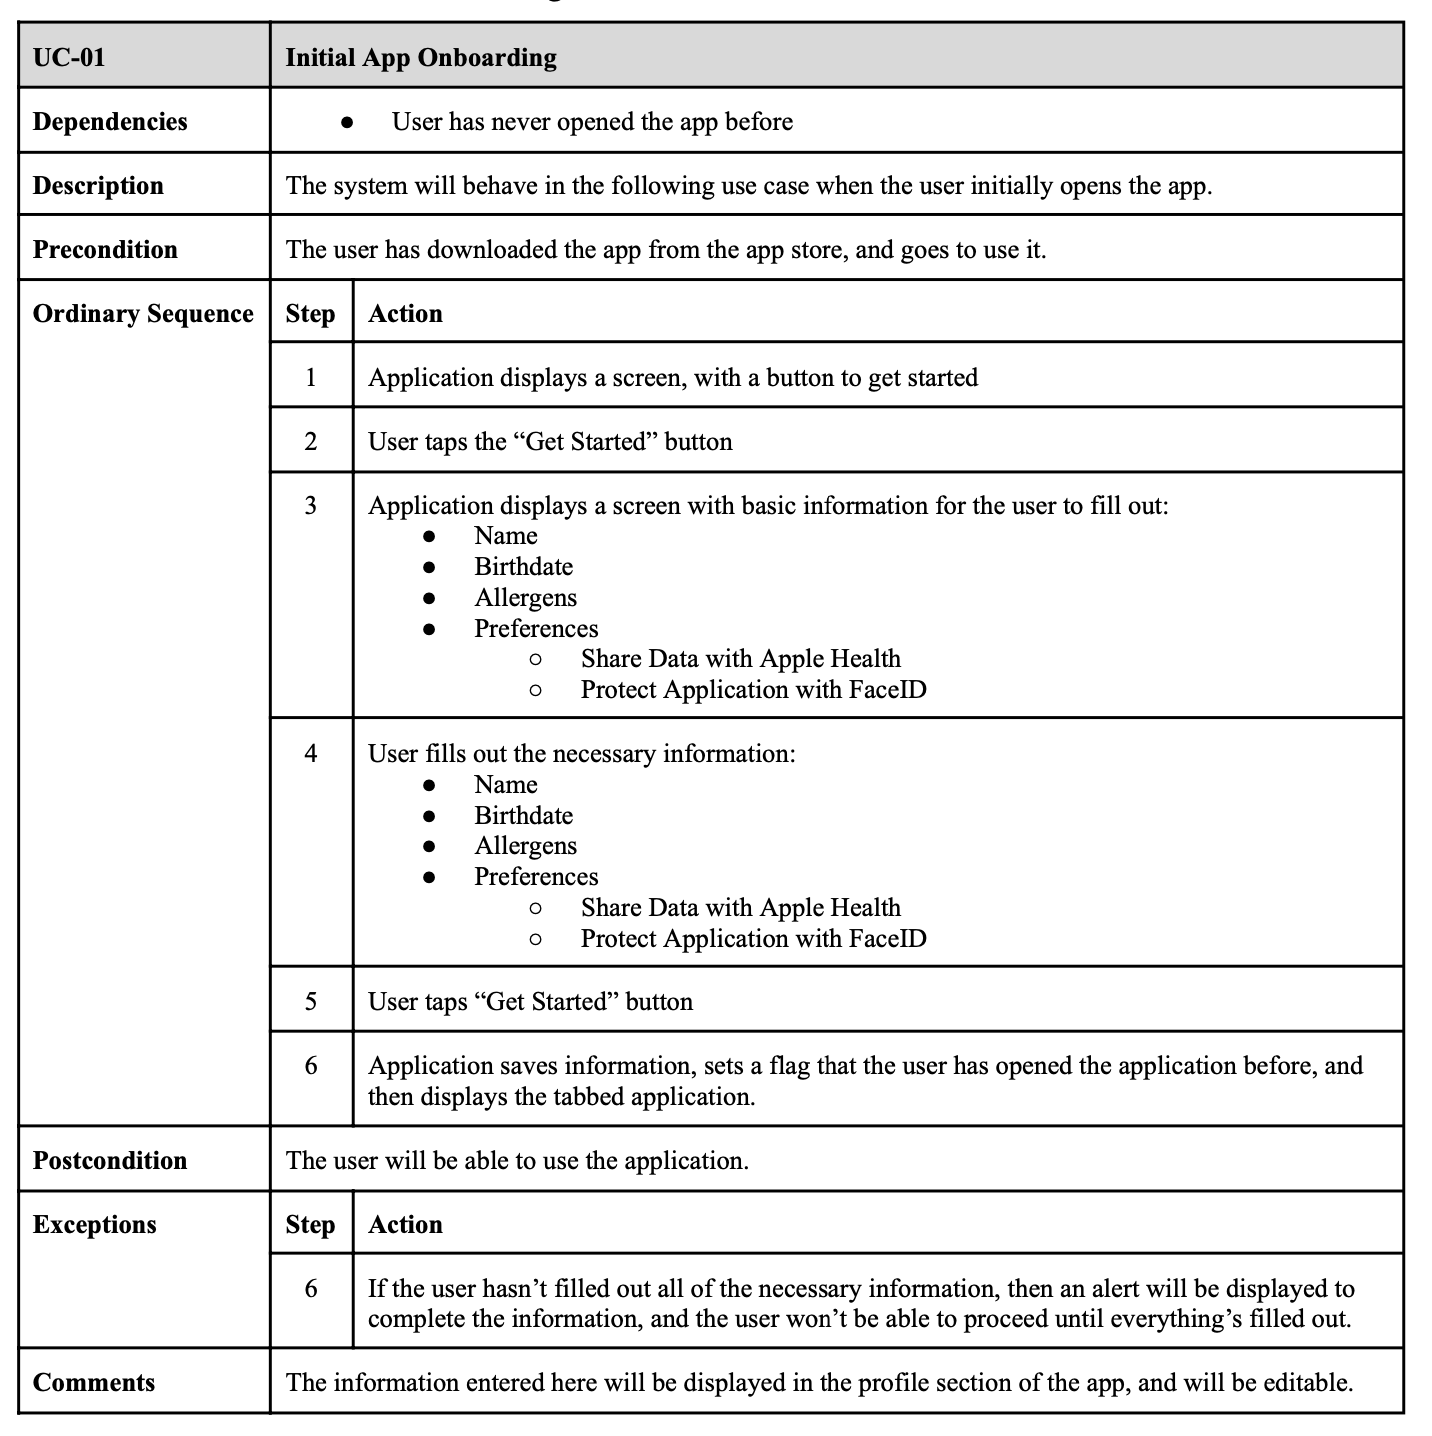
\includegraphics[width=1\linewidth]{thesis//chapters//images/uc-01.png}
    \caption{Use Case 01: Initial App Onboarding}
    \label{fig:uc01-table}
\end{table}

\begin{table} [H]
    \centering
    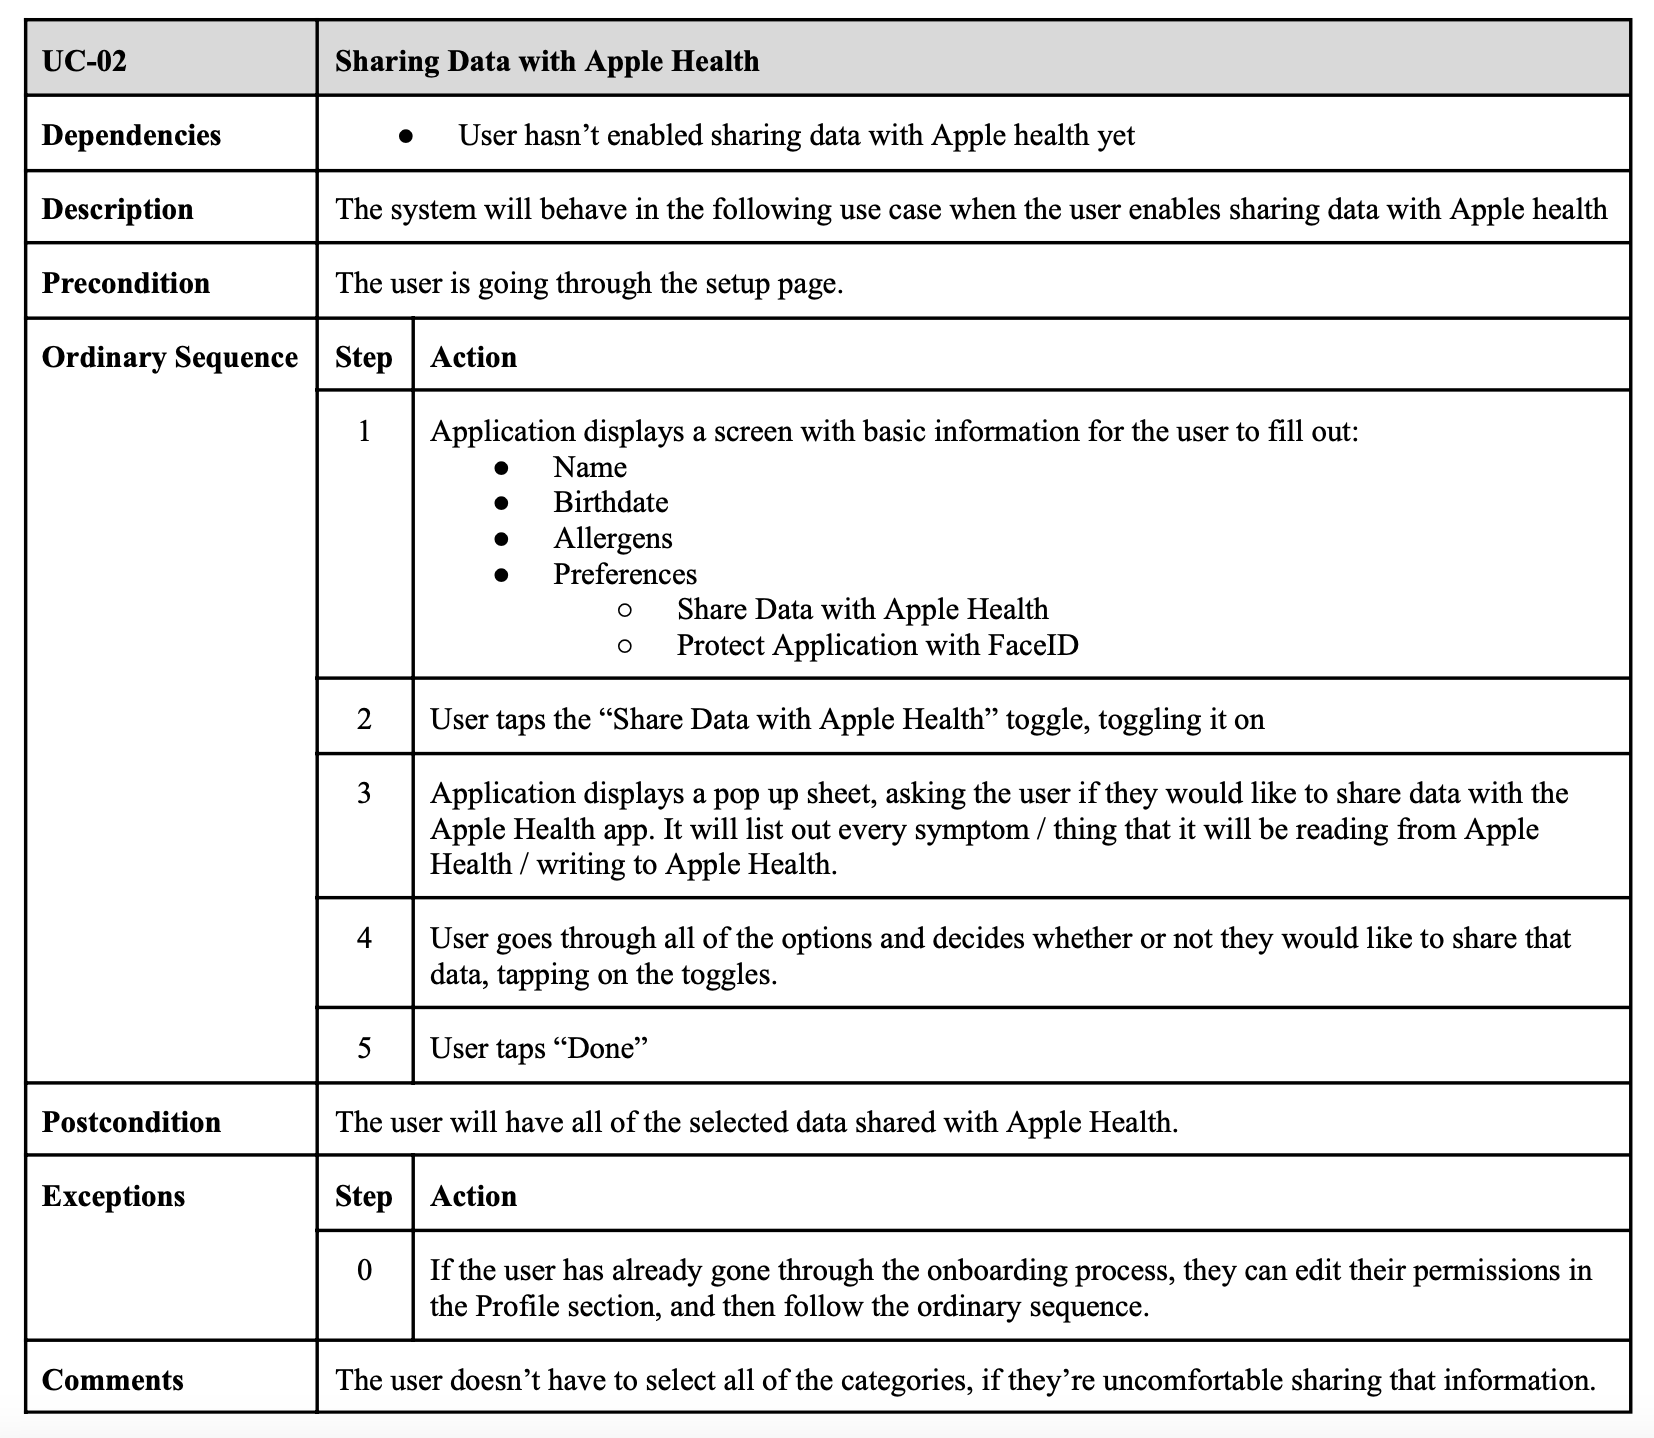
\includegraphics[width=1\linewidth]{thesis//chapters//images/uc-02.png}
    \caption{Use Case 02: Sharing Data with Apple Health}
    \label{fig:uc02-table}
\end{table}

\begin{figure} [H]
    \centering
    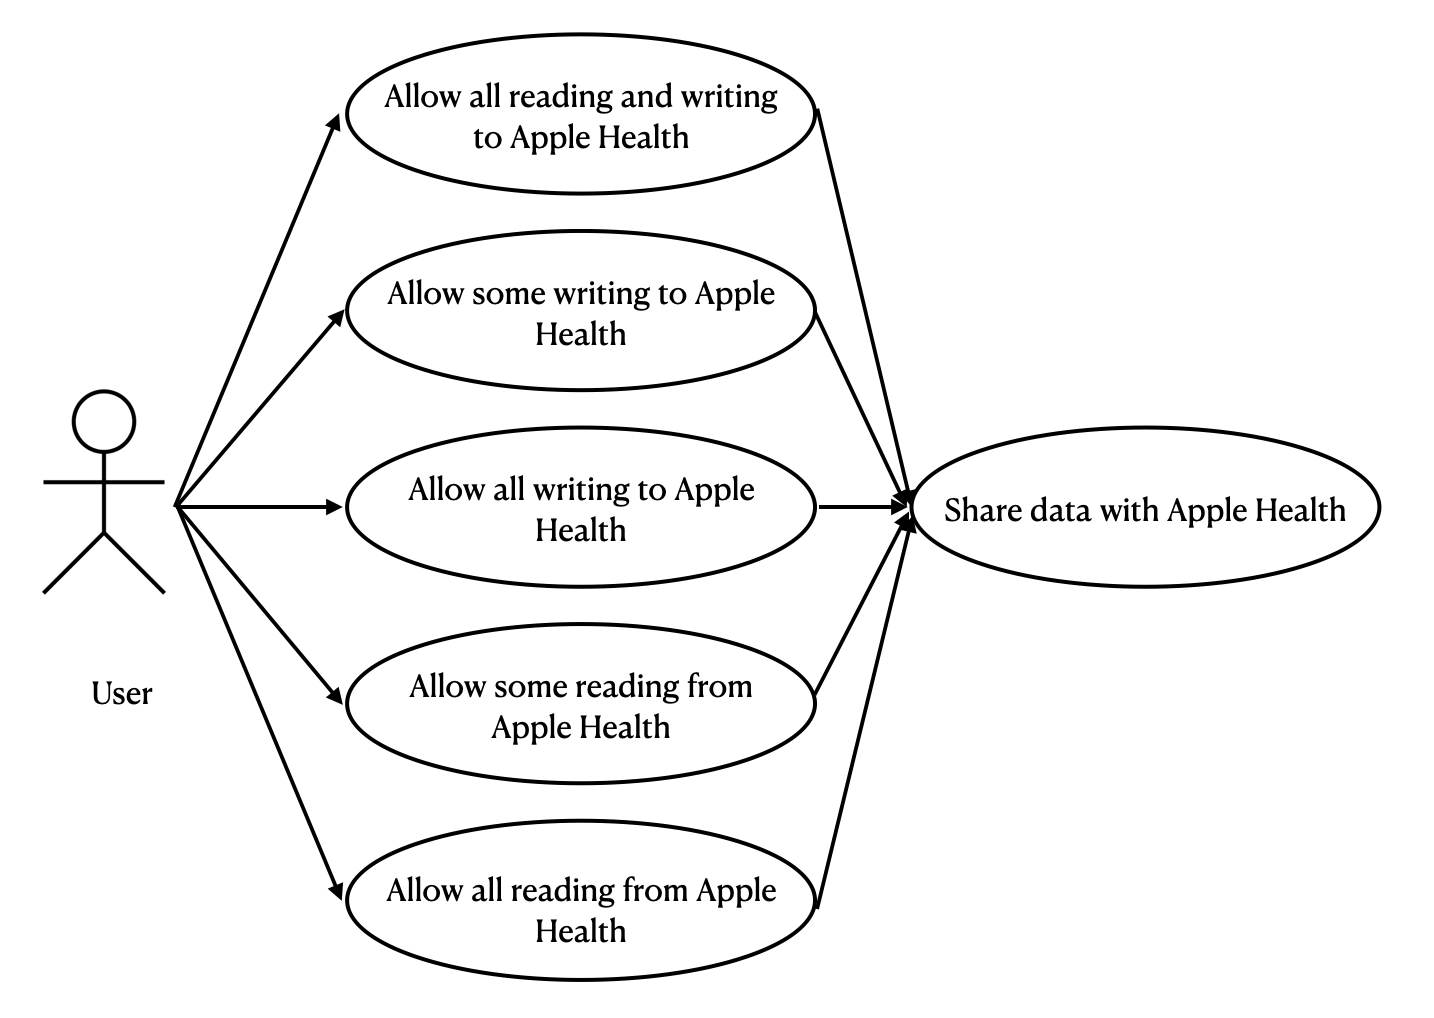
\includegraphics[width=0.75\linewidth]{thesis//chapters//images/uc-02-visual.png}
    \caption{Use Case 02: Visual Diagram}
    \label{fig:uc02-visual-diagram}
\end{figure}

\begin{table} [H]
    \centering
    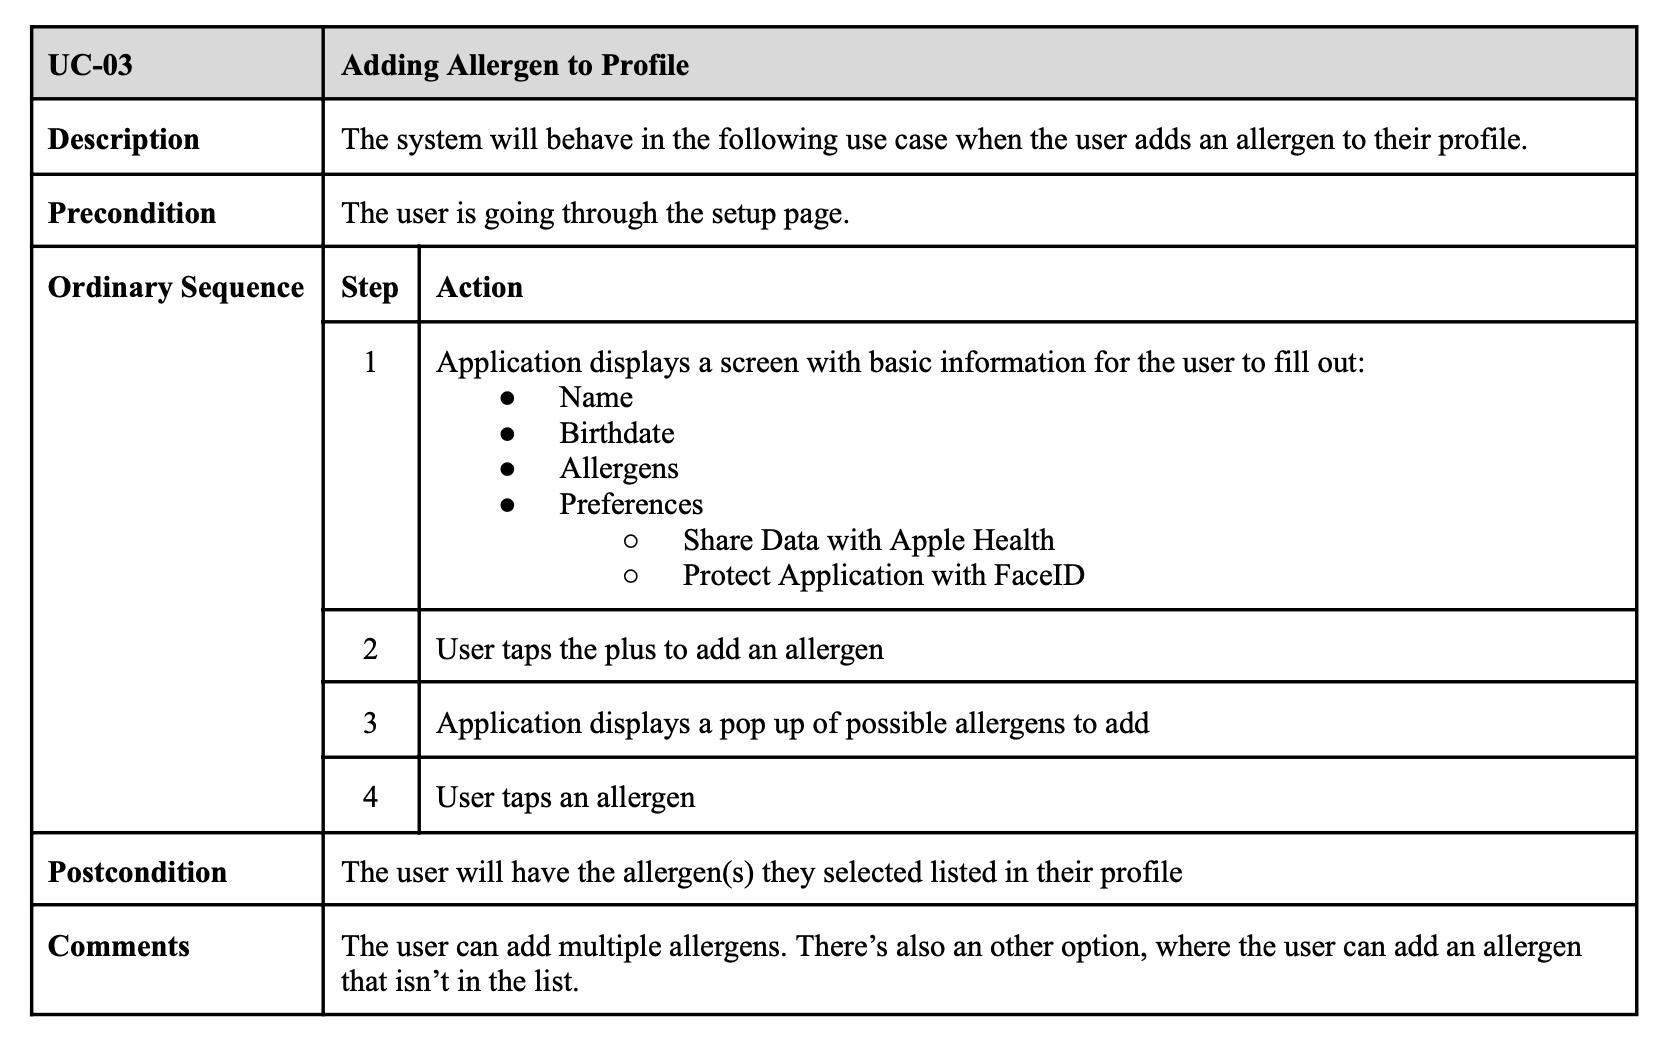
\includegraphics[width=1\linewidth]{thesis//chapters//images/uc-03.png}
    \caption{Use Case 03: Adding Allergen to Profile}
    \label{fig:uc03-table}
\end{table}

\begin{figure} [H]
    \centering
    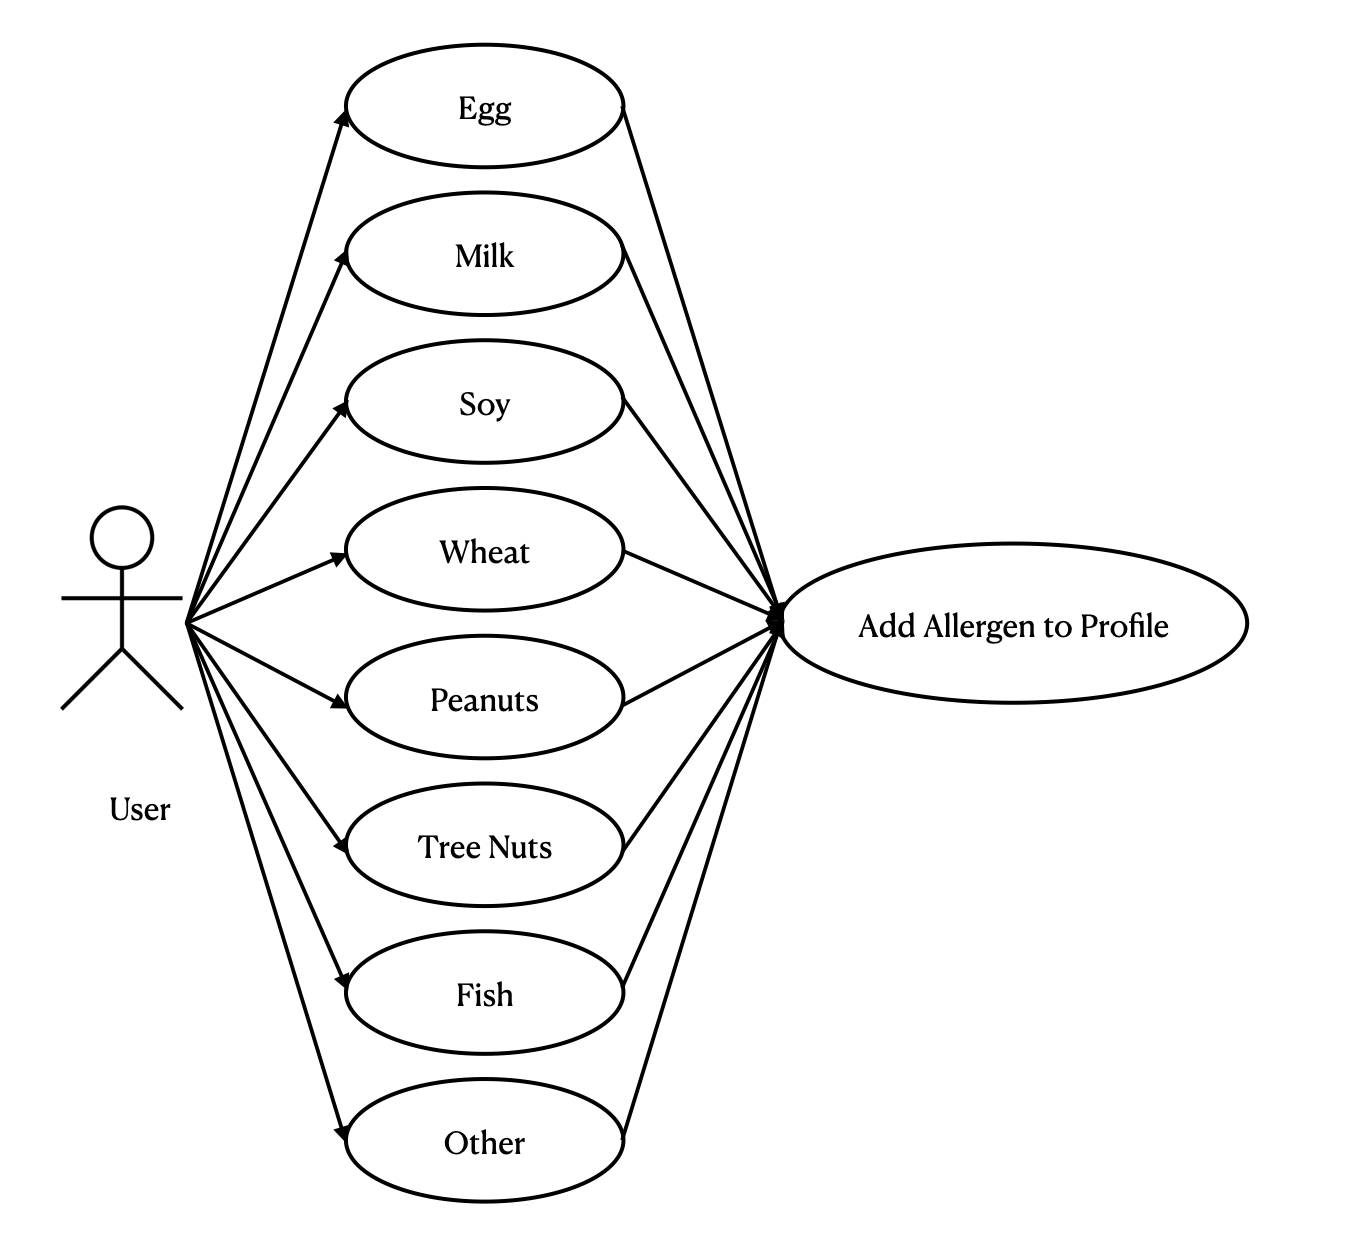
\includegraphics[width=0.75\linewidth]{thesis//chapters//images/uc-03-visual.png}
    \caption{Use Case 03: Visual Diagram}
    \label{fig:uc03-visual-diagram}
\end{figure}

\begin{table} [H]
    \centering
    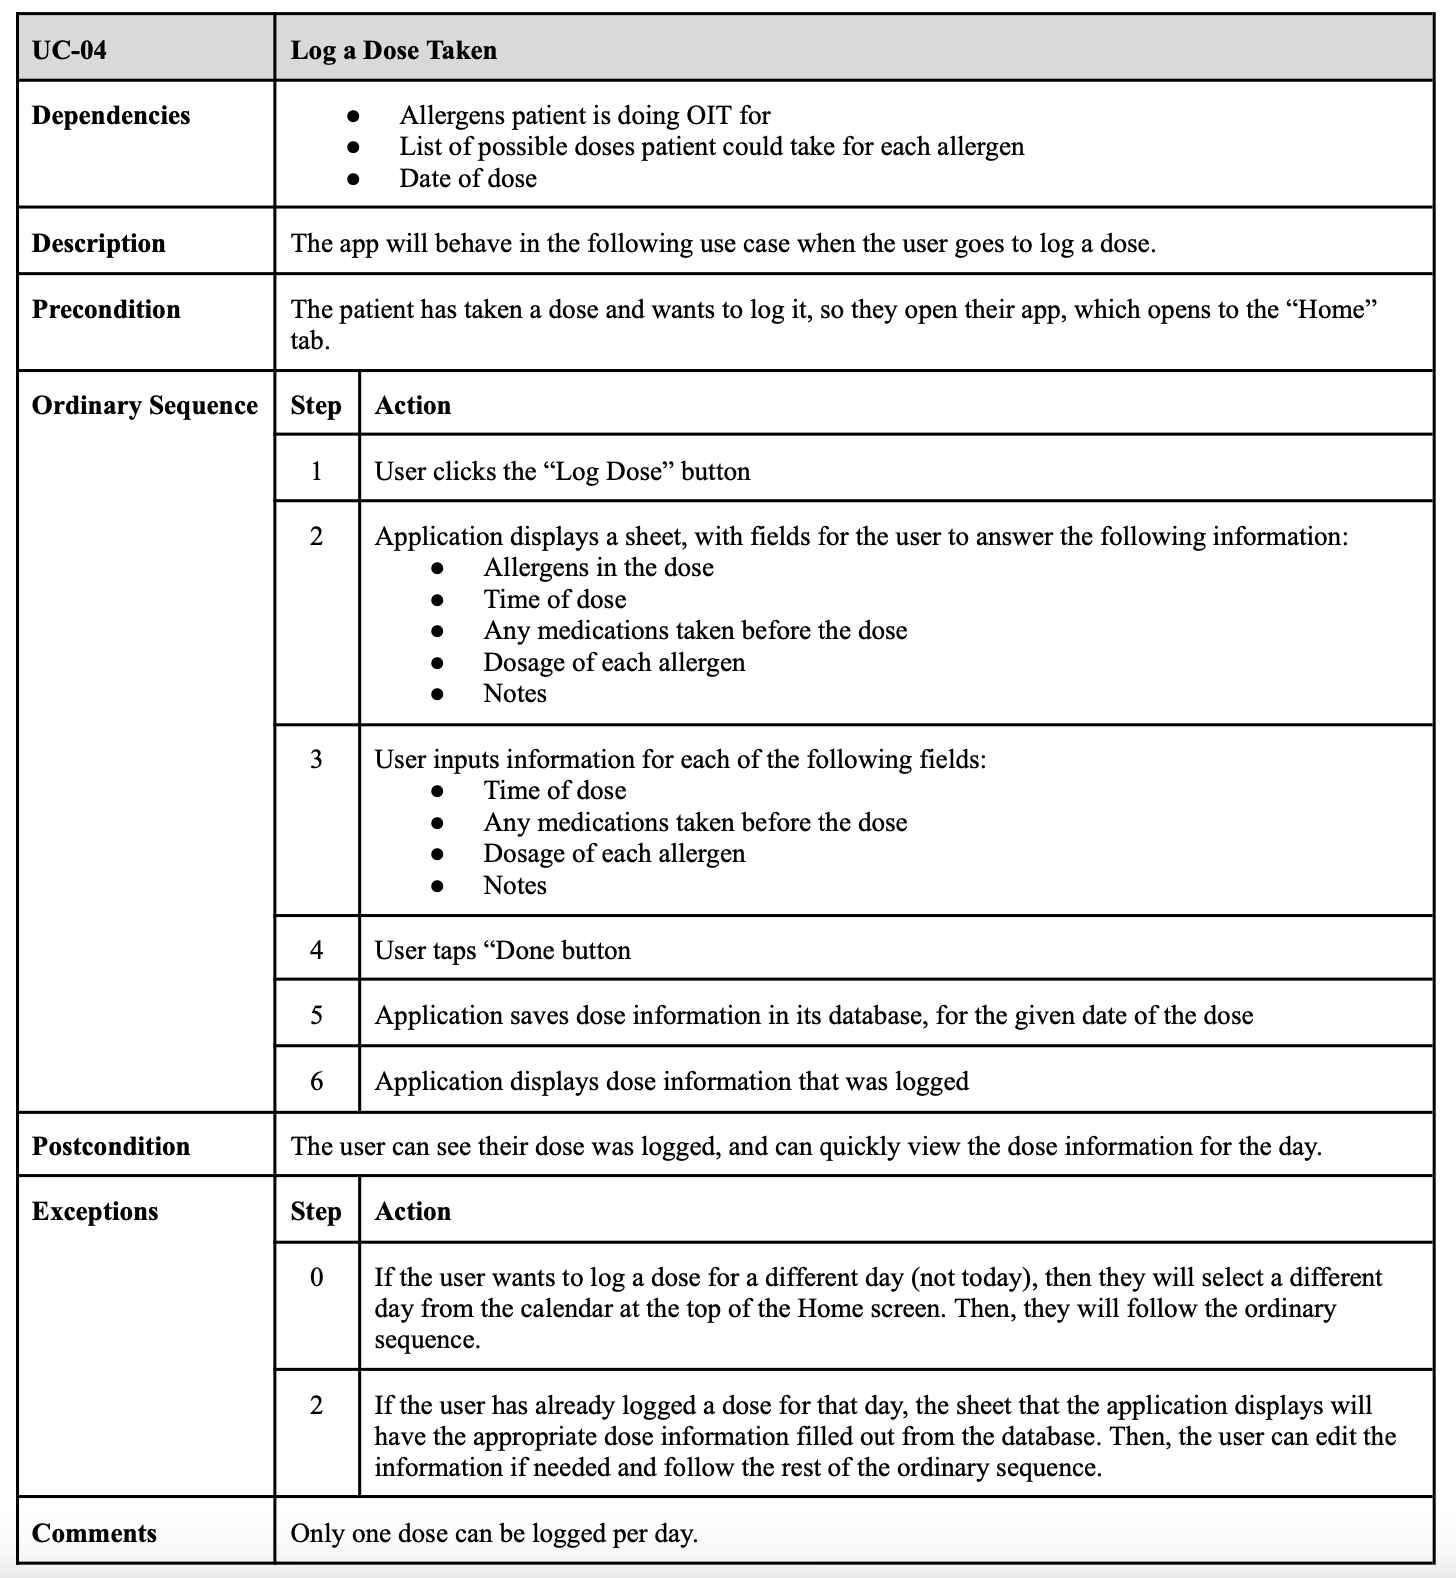
\includegraphics[width=1\linewidth]{thesis//chapters//images/uc-04.png}
    \caption{Use Case 04: Log a Dose Taken}
    \label{fig:uc04-table}
\end{table}

\begin{figure} [H]
    \centering
    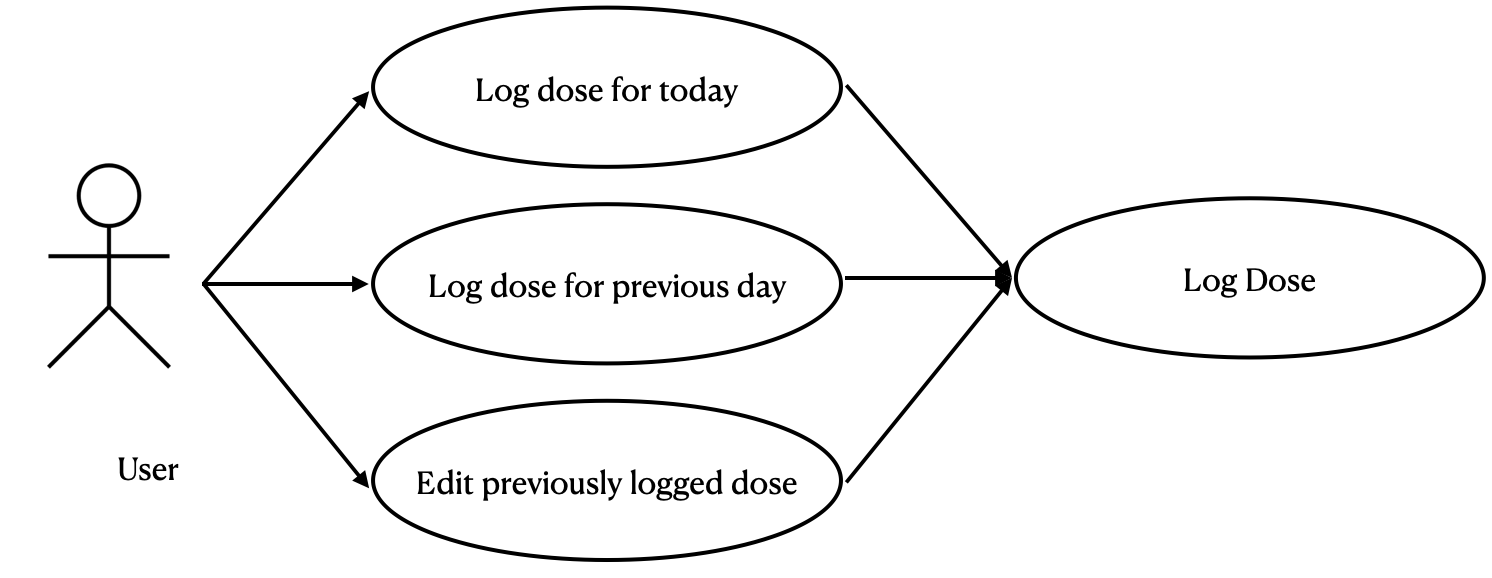
\includegraphics[width=0.75\linewidth]{thesis//chapters//images/uc-04-visual.png}
    \caption{Use Case 04: Visual Diagram}
    \label{fig:uc04-visual-diagram}
\end{figure}

\begin{table} [H]
    \centering
    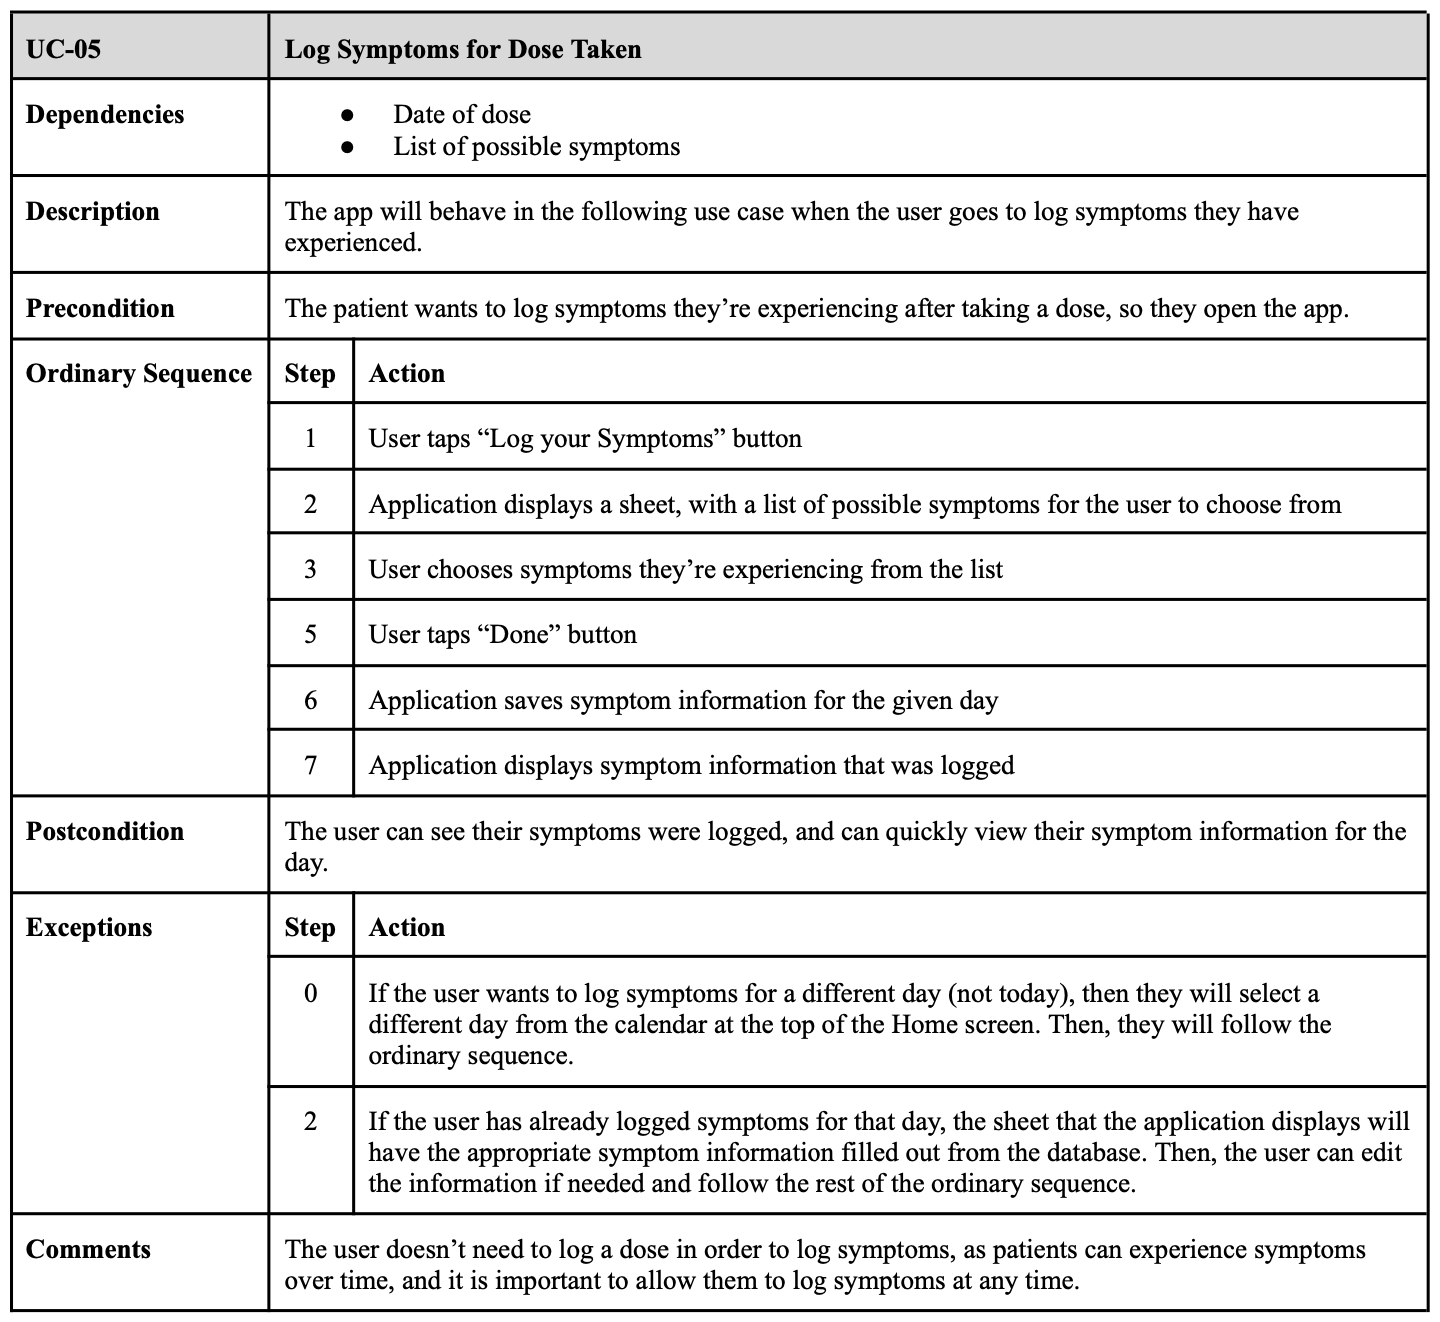
\includegraphics[width=1\linewidth]{uc-05.png}
    \caption{Use Case 05: Log Symptoms for Dose Taken}
    \label{fig:uc05-table}
\end{table}

\begin{figure} [H]
    \centering
    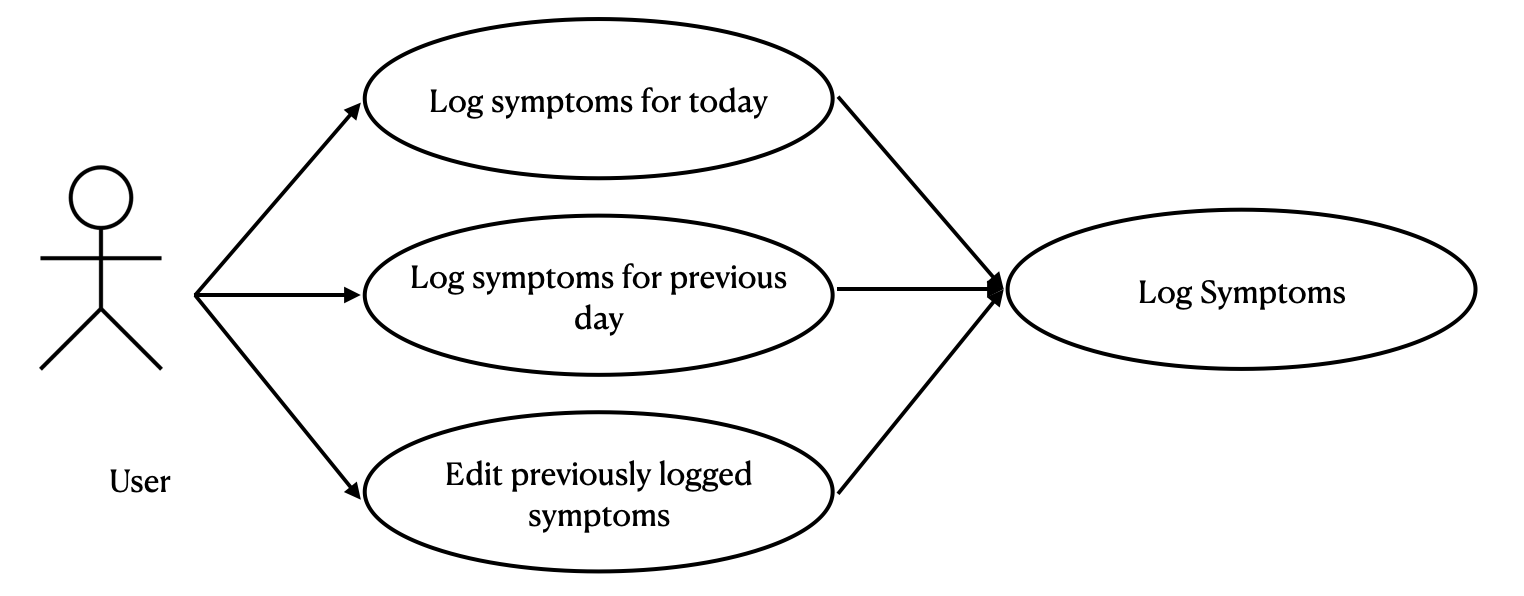
\includegraphics[width=0.75\linewidth]{thesis//chapters//images/uc-05-visual.png}
    \caption{Use Case 05: Visual Diagram}
    \label{fig:uc05-visual-diagram}
\end{figure}

\begin{table} [H]
    \centering
    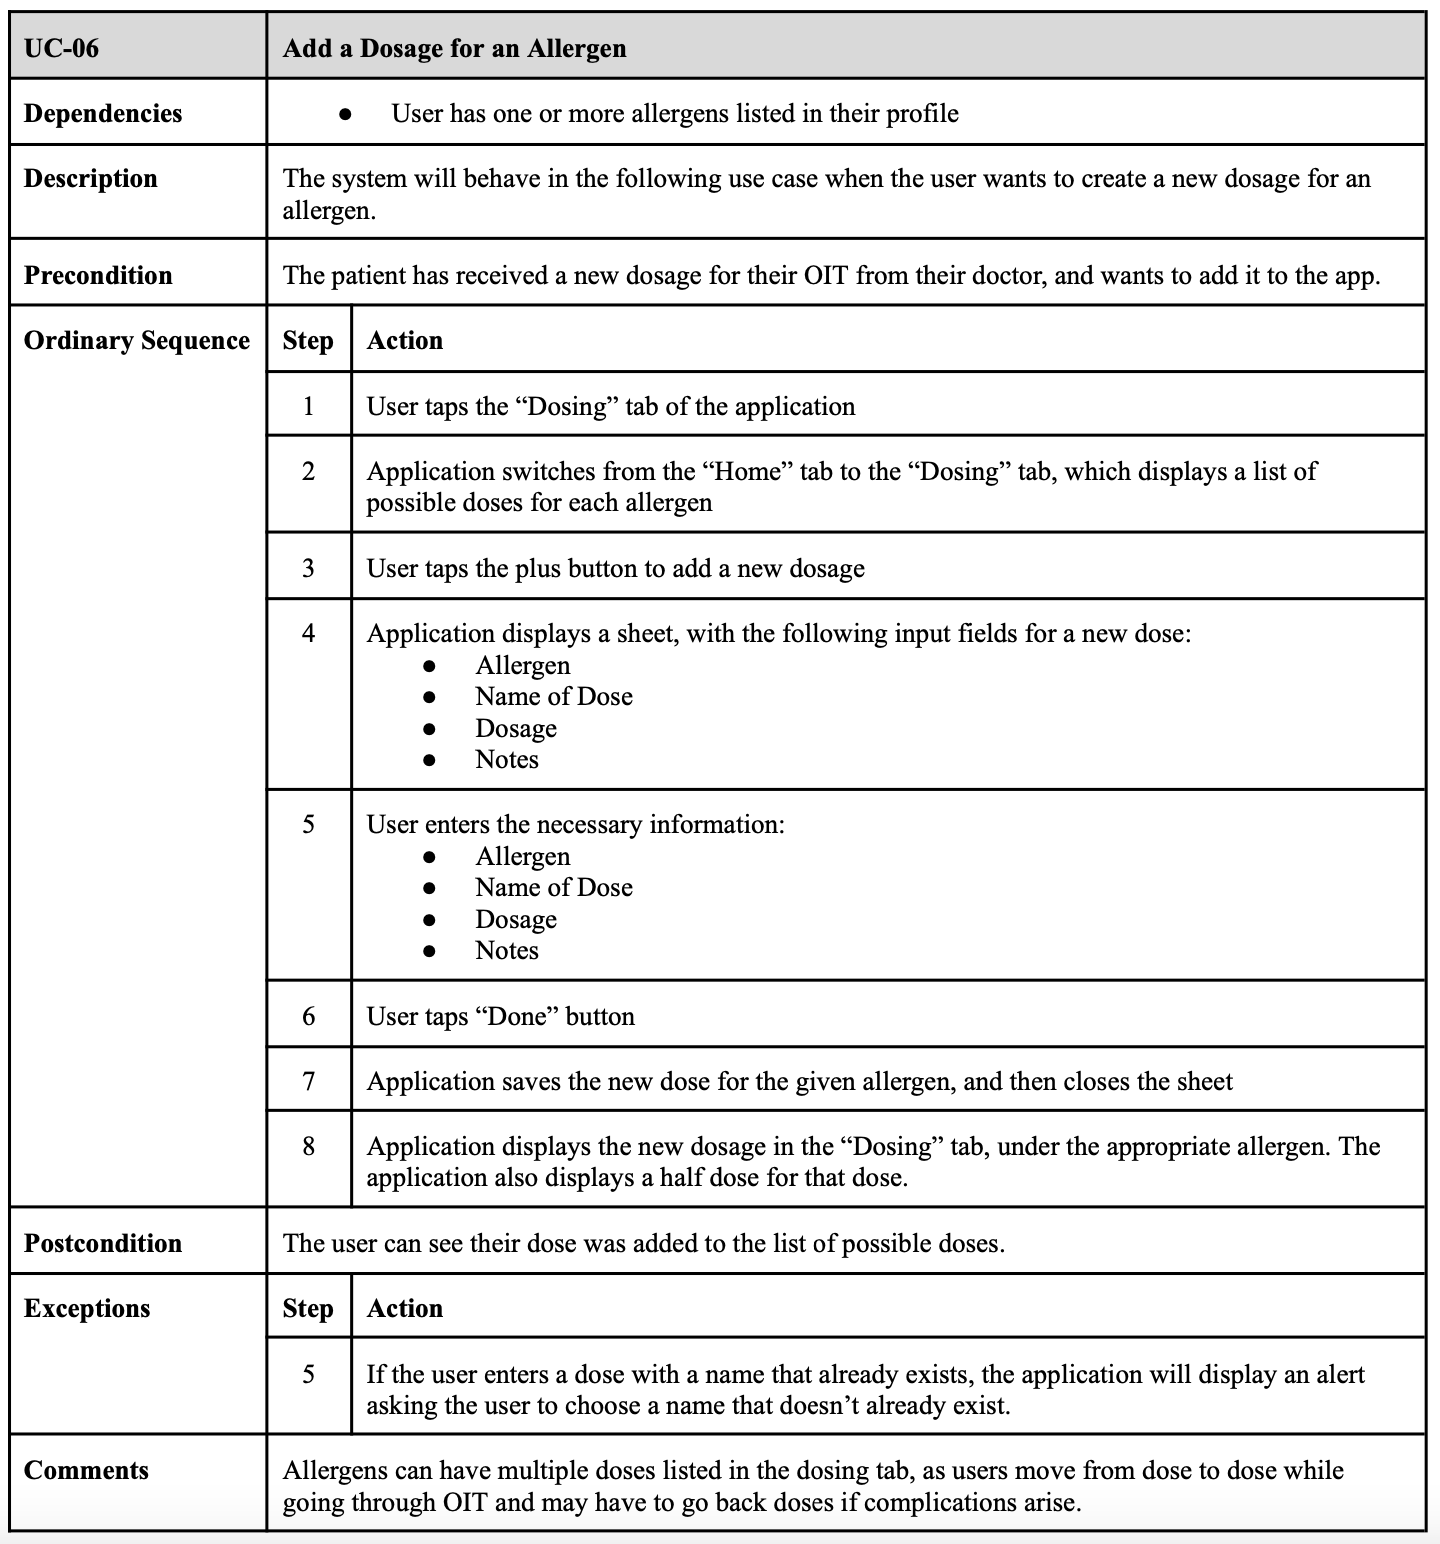
\includegraphics[width=1\linewidth]{uc-06.png}
    \caption{Use Case 06: Add a Dosage for an Allergen}
    \label{fig:uc06-table}
\end{table}

\begin{table} [H]
    \centering
    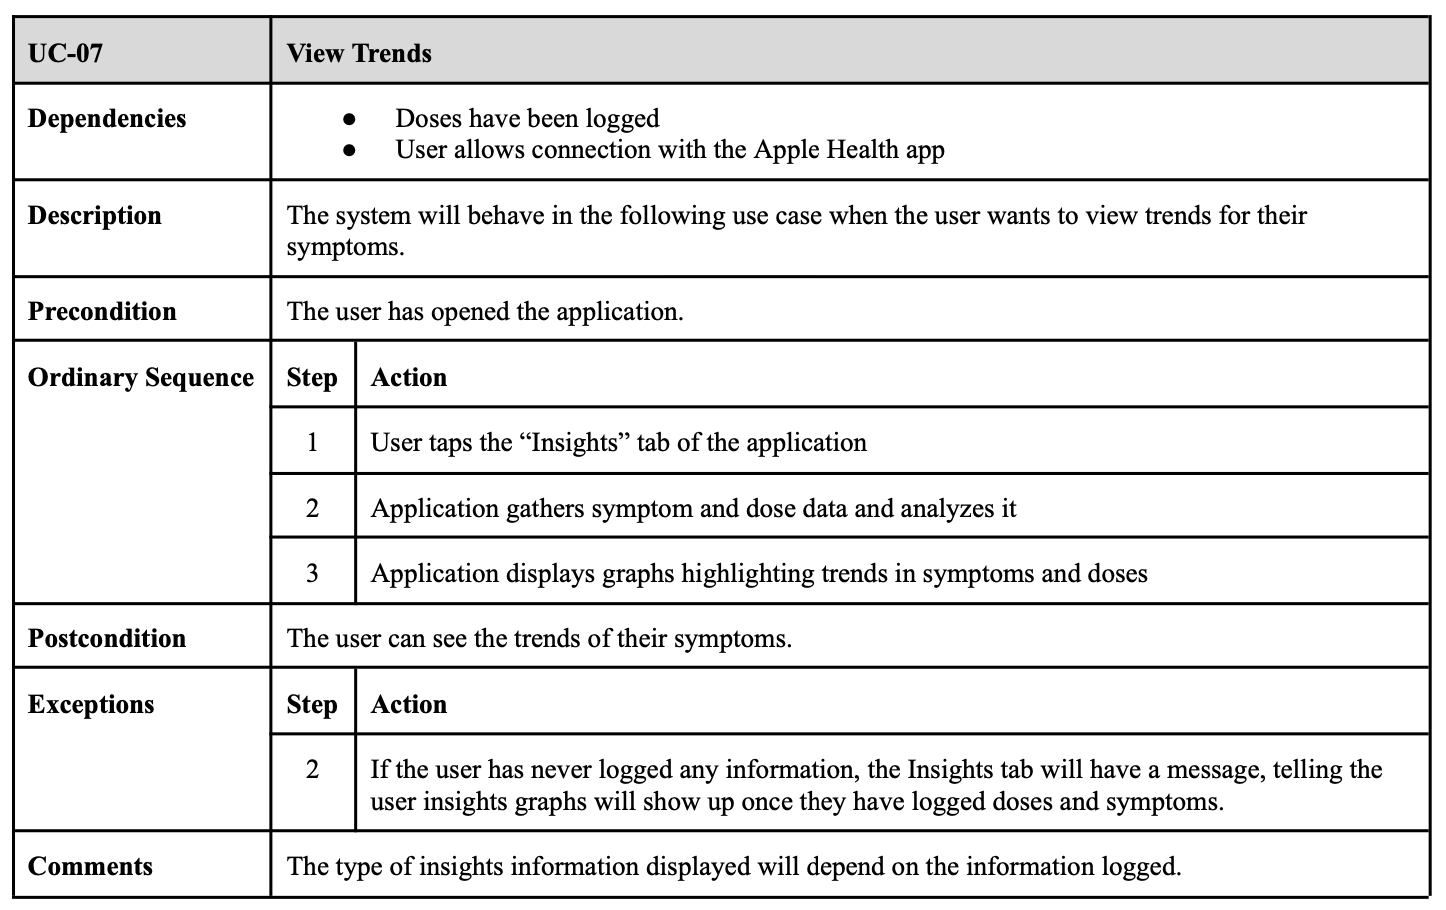
\includegraphics[width=1\linewidth]{thesis//chapters//images/uc-07.png}
    \caption{Use Case 07: View Trends}
    \label{fig:uc07-table}
\end{table}

\begin{table} [H]
    \centering
    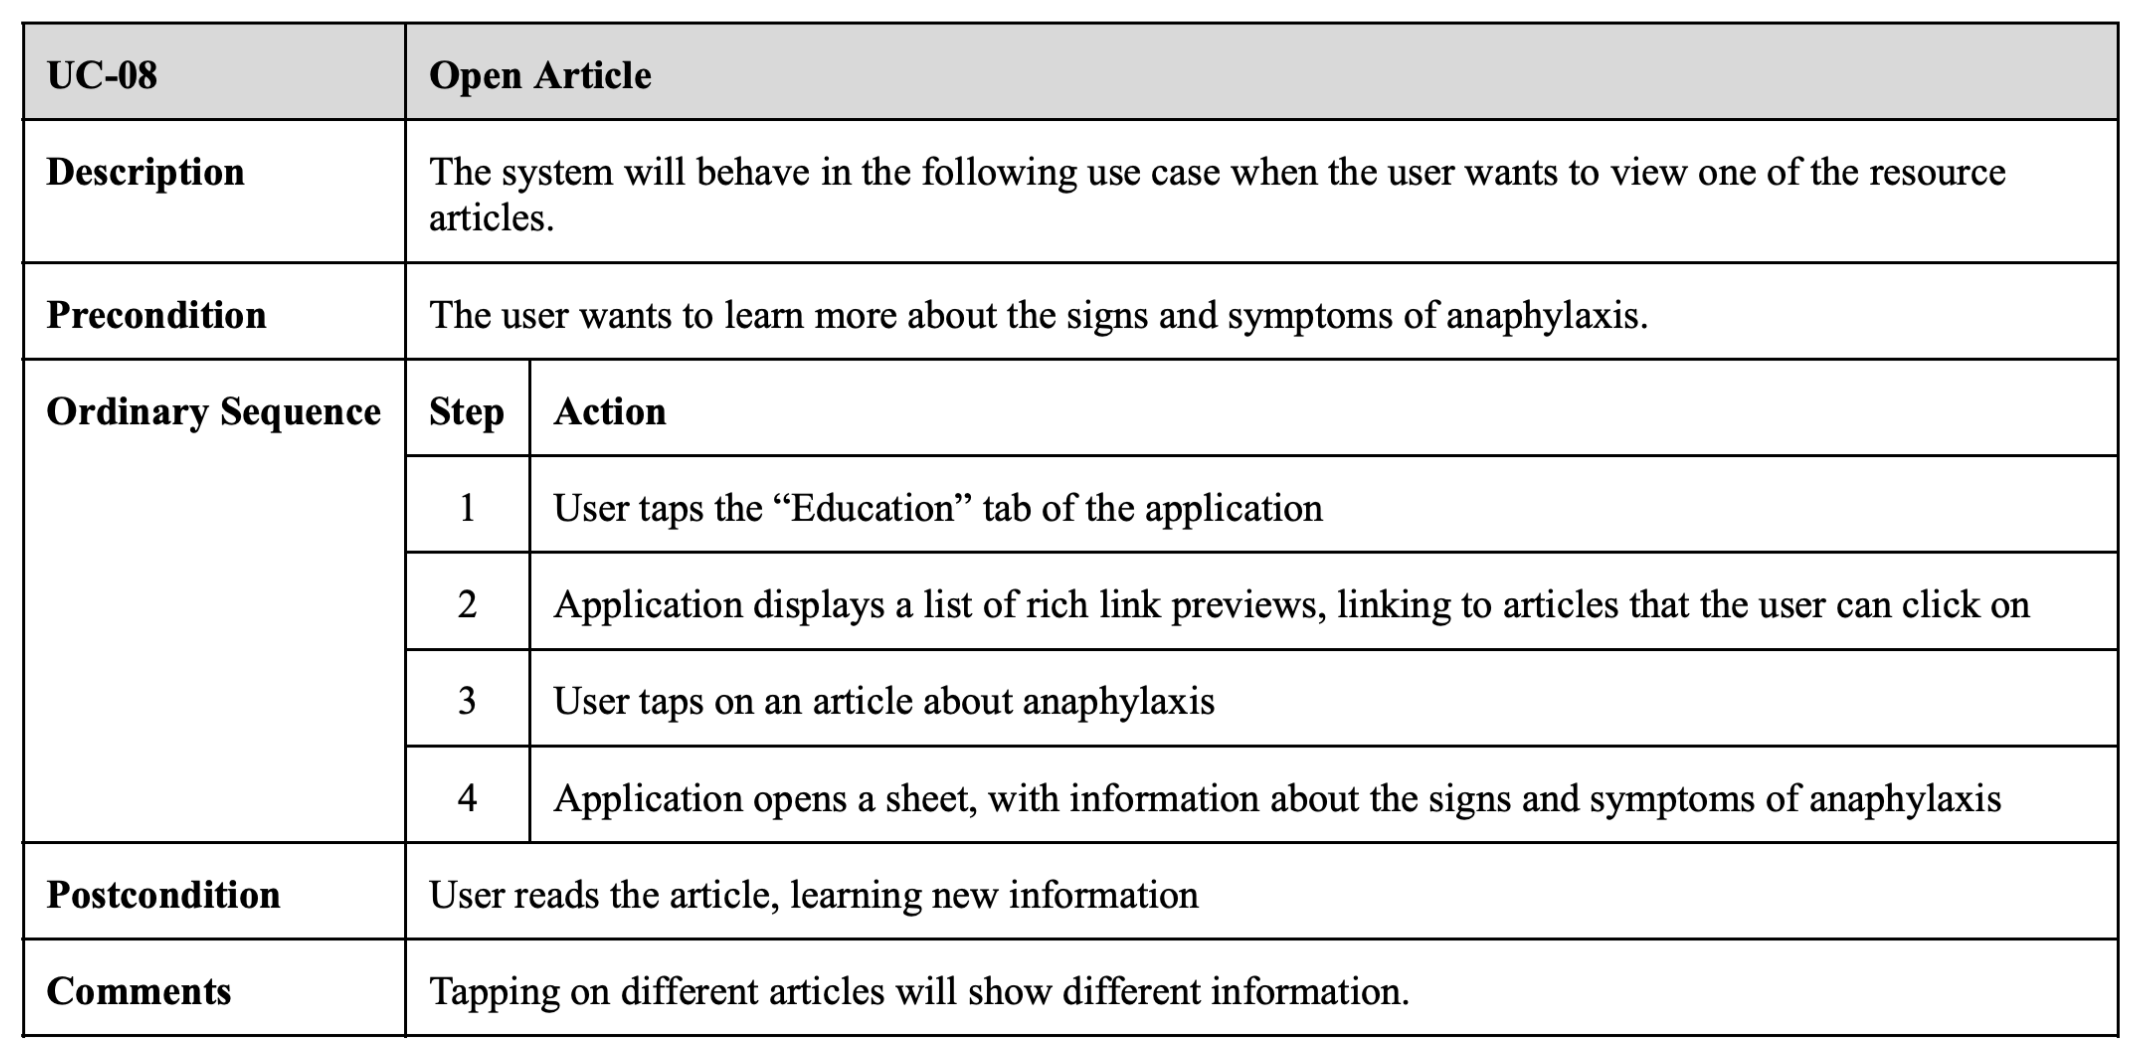
\includegraphics[width=1\linewidth]{thesis//chapters//images/uc-08.png}
    \caption{Use Case 08: Open Article}
    \label{fig:uc08-table}
\end{table}

\begin{table} [H]
    \centering
    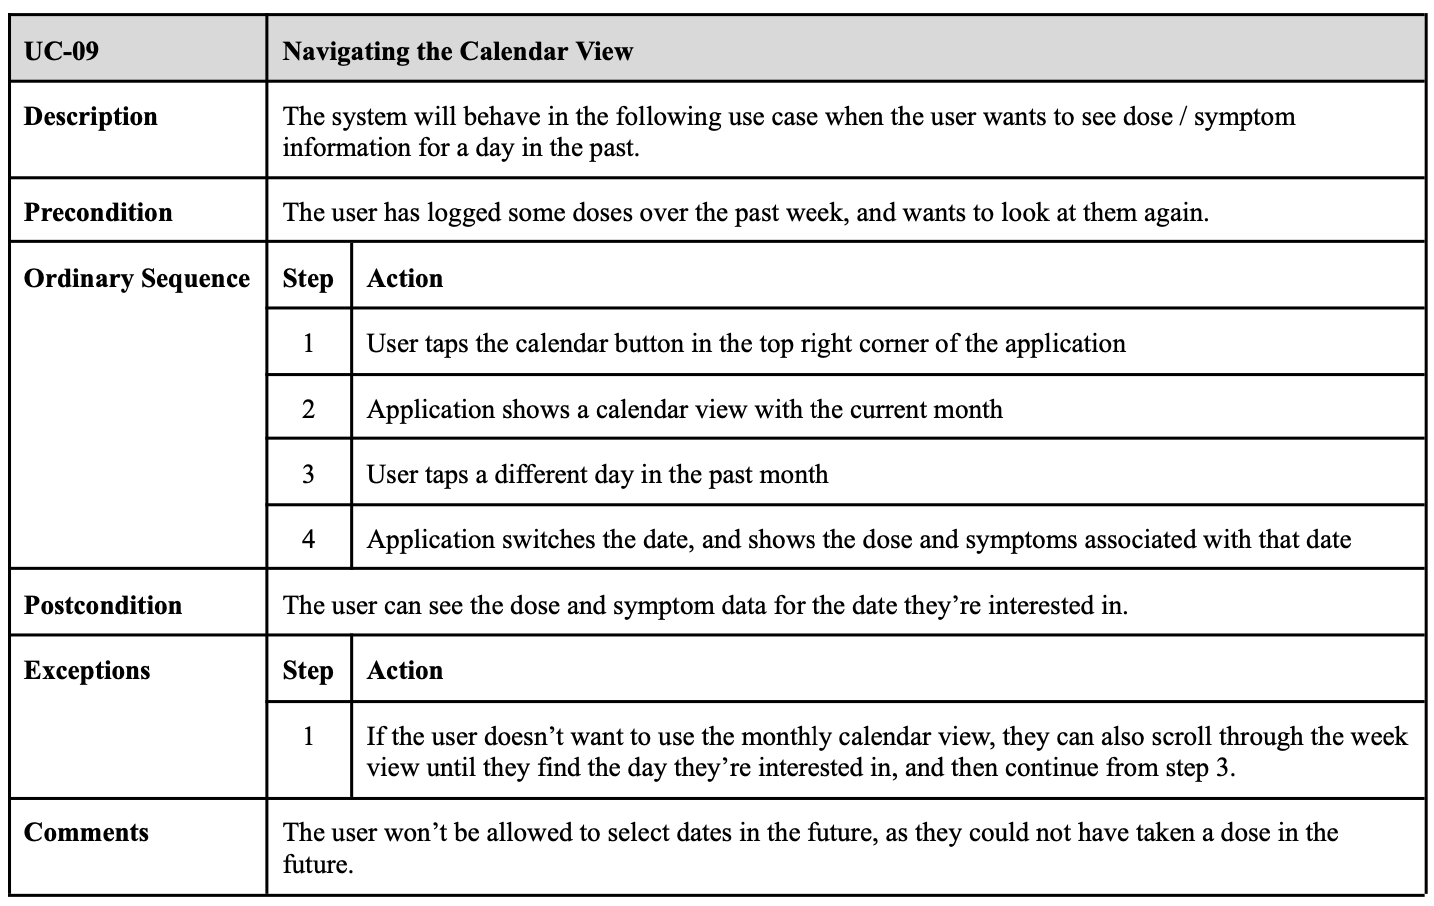
\includegraphics[width=1\linewidth]{thesis//chapters//images/uc-09.png}
    \caption{Use Case 09: Navigating the Calendar View}
    \label{fig:uc09-table}
\end{table}

\begin{figure} [H]
    \centering
    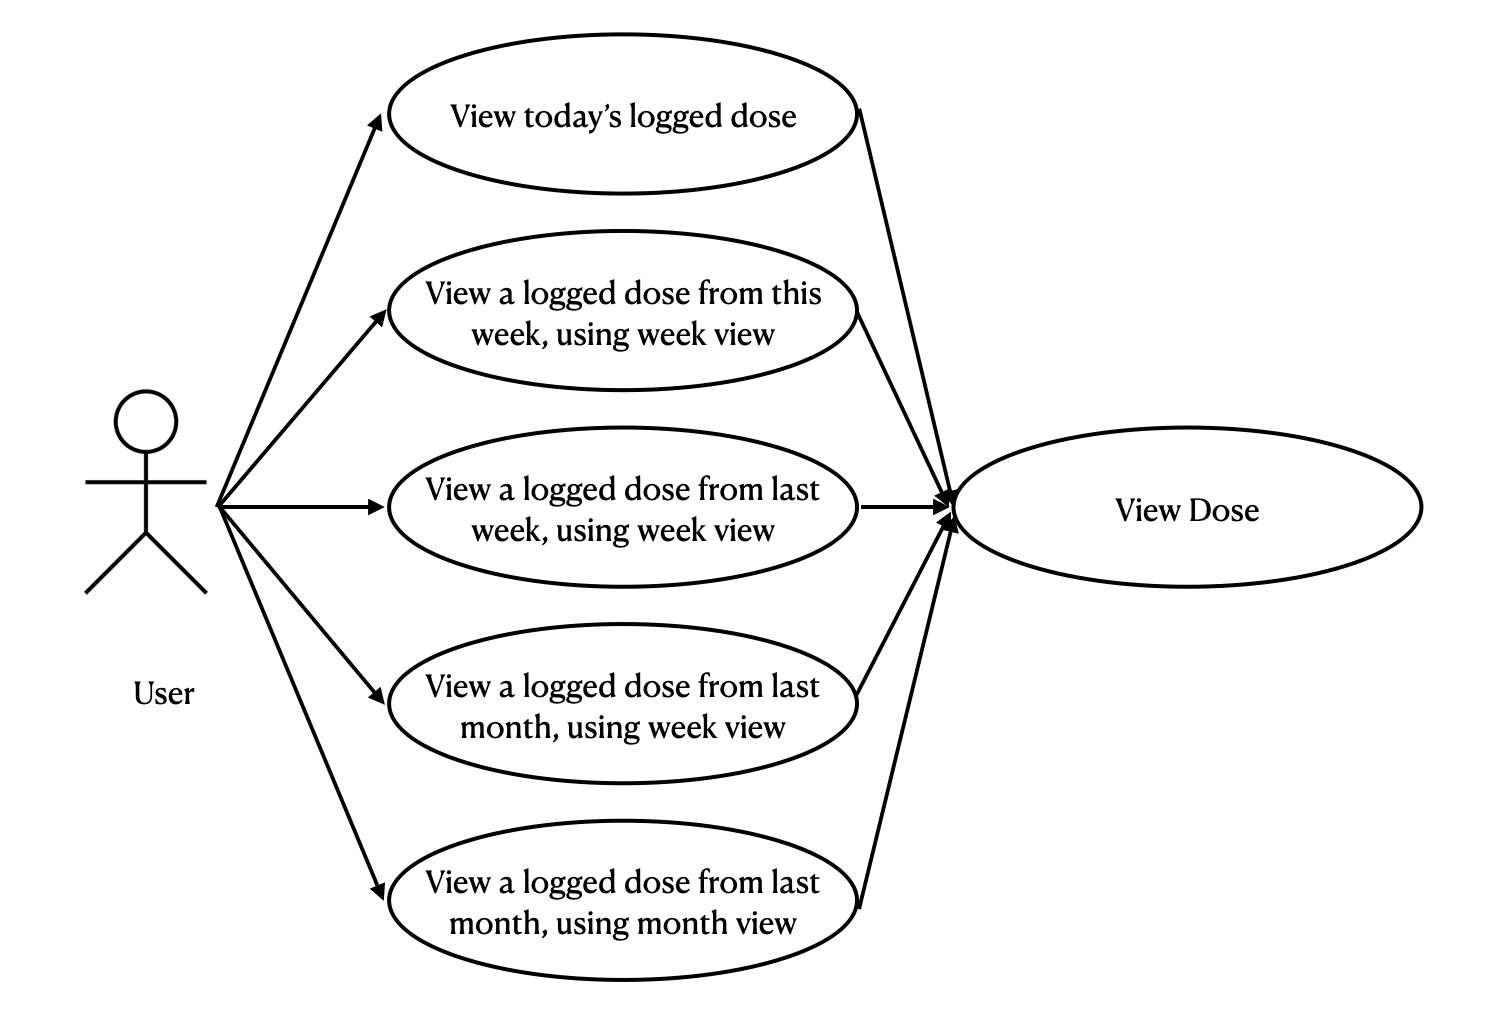
\includegraphics[width=0.75\linewidth]{thesis//chapters//images/uc-09-visual1.png}
    \caption{Use Case 09: Visual Diagram 1}
    \label{fig:uc09-visual-diagram1}
\end{figure}

\begin{figure} [H]
    \centering
    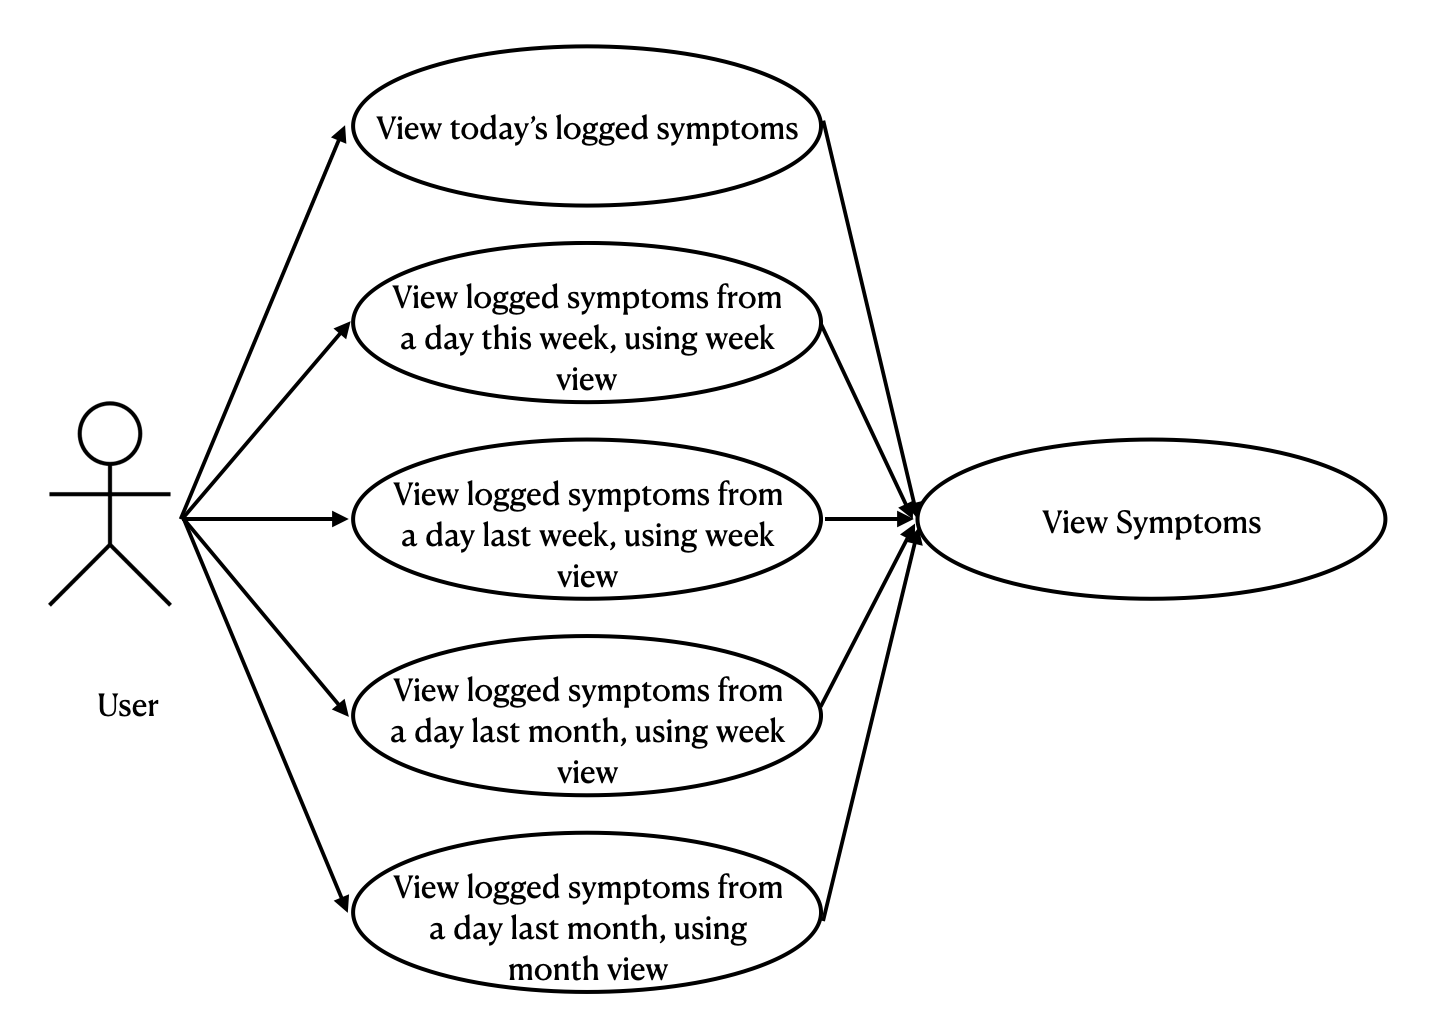
\includegraphics[width=0.75\linewidth]{thesis//chapters//images/uc-09-visual2.png}
    \caption{Use Case 09: Visual Diagram 2}
    \label{fig:uc09-visual-diagram2}
\end{figure}




\chapter{Research}

While I know a lot about OIT from my own experiences, it was important that I thoroughly researched the topic before creating my initial design – especially because OIT is a new, emerging treatment and isn't standardized, so it's different from clinic to clinic. This chapter outlines my research on OIT, shedding light on its definition and mechanisms, as well as the initial advice I received from allergists and immunologists in the field.

\section{Research}

\subsection{Background}
Oral Immunotherapy has exhibited remarkable efficacy in addressing a spectrum of food allergies, including peanuts, tree nuts, milk, and eggs. The impact on patients' quality of life is profound, offering hope and tangible relief. As revealed by recent studies, the success of OIT is particularly notable in young patients, especially those under 3 years old. For example, a study found that young patients demonstrate the highest success rates in OIT, showcasing the treatment's potential for transformative outcomes in this age group \cite{Blumchen}.

The mechanistic underpinnings of OIT unfold within the intricate interactions of the immune system. Research indicates that carefully administered doses of allergens through OIT orchestrate a controlled immune response \cite{Nairn}. This calibrated exposure triggers the production of regulatory T cells and other immune modulators, facilitating a shift from hypersensitivity to a more tolerant state. Such immune modulation is crucial for the success of OIT, and understanding these processes informs the app design to ensure patients comprehend the science behind their treatment. 

\subsection{The Patient's Journey}

The OIT patient journey is a nuanced process, beginning with a meticulous selection phase that takes into account factors such as age, allergy severity, and overall health. Recent research has highlighted the critical role of comprehensive assessments and diagnosis in guiding a tailored treatment plan. For instance, a study found that the success of OIT is intricately linked to understanding the specific allergens triggering reactions in individual patients \cite{Dominguez}. This research underscores the importance of incorporating detailed allergy testing and evaluations into the app to guide users through a personalized OIT journey.

The carefully designed OIT protocol involves a gradual introduction of allergens in controlled doses, with customization based on individual needs. Data from ongoing studies emphasizes that adapting the frequency and intensity of allergen doses to individual responses is essential for the efficacy of OIT. Incorporating this insight into the app ensures that users have a clear understanding of the gradual exposure process, fostering adherence and positive engagement.

\subsection{Predosing Medications and Precautions}

Predosing medications play a pivotal role in preparing patients for controlled allergen exposure during OIT. Recent findings, as seen in various clinical studies, underscore the importance of this precautionary step. For example, research suggests that administering medications, such as antihistamines, mitigates the risk of immediate allergic reactions, enhancing the overall safety profile of OIT \cite{Gilbert}. This crucial insight informs the app's design to include features that remind users about predosing medications and educate them on their significance in ensuring a smooth OIT progression.

The close monitoring of patient responses to predosing medications, as supported by research, further emphasizes the adaptability of treatment plans to individual sensitivities. Integrating tools in the app that allow users to track and report their responses ensures a more personalized OIT experience, aligning with the variability observed in patient reactions.

\subsection{Adherence to Strict Rules and Lifestyle Adjustments}

The path to successful Oral Immunotherapy involves a commitment to adherence to strict rules and lifestyle adjustments. Patients partaking in OIT are often advised to refrain from vigorous exercise after each session and abstain from alcohol during the treatment period. Research has demonstrated that these seemingly restrictive measures are integral to the safety and efficacy of the treatment \cite{Dominguez}.

For instance, ongoing studies have shown that adherence to guidelines significantly influences the success of OIT, reducing the risk of adverse reactions. This underscores the personalized nature of OIT, emphasizing the need for patients to actively engage in their own care. The app design takes inspiration from this research, incorporating features that not only educate users on the importance of adherence but also provide tools for tracking and maintaining lifestyle adjustments.

\subsection{Highly Personalized Treatment Plans}

A key takeaway from the research is the highly personalized nature of OIT treatment plans. Recent studies have emphasized that the success of OIT lies in recognizing the uniqueness of each patient's journey. Treatment plans are meticulously crafted based on factors such as age, medical history, specific allergens, and overall health. This tailored approach allows for adjustments in allergen dose frequency and intensity, ensuring effective and well-tolerated progress.

For example, ongoing research has shown that individualized treatment plans significantly contribute to positive outcomes in OIT. Patients progress through therapy at a pace that is both effective and well-tolerated, reducing the risk of adverse reactions. The individualized nature of OIT reflects its commitment to providing bespoke solutions, acknowledging the diversity of allergic conditions and accommodating variations in the treatment process. The app, inspired by this research, prioritizes customization, offering users a personalized roadmap for their OIT journey.

\section{Consultation with Immunologists}

After thoroughly researching OIT, the natural next step in my research and design process was to bring my app idea to doctors, and garner their advice. I collaborated with top immunologists from The Children's Hospital of Philadelphia, Mt. Sinai Hospital, and Stanford Medicine to ensure that my application aligns with expert advice and industry best practices. Here are some key pieces of advice I received:

\begin{itemize}
    \item \textbf{Pop Up to Seek Medical Care: }Immunologists recommended displaying a pop-up notification encouraging users to "Call your doctor" or "Call 911" if any aspect of their symptoms raises concerns.
    \item \textbf{Engagement through Notifications: }Immunologists emphasized the importance of subtle reminders, such as "Did you take your dose today?" These notifications not only promote adherence to treatment plans but also serve as a gentle nudge towards consistent health practices.
    \item \textbf{Emergency Preparedness: }Immunologists advised incorporating an innovative feature allowing users to upload images of their emergency action plans to the 'Resources' section. This practical addition ensures that critical information is readily accessible, fostering a sense of empowerment in navigating unforeseen health scenarios.
    \item \textbf{Educational Prompts:} In the realm of education, immunologists recommended maintaining a delicate balance to avoid offering explicit medical advice. Instead, the app should gently prompt users with thought-provoking questions like, "Did you ask your doctor about this? Or that?" This approach encourages informed discussions with healthcare providers, fostering a proactive and engaged patient community.
    \item \textbf{Autoinjector Management: }Recognizing the prevalence of autoinjectors in allergy management, immunologists suggested a dedicated section providing functionality to check the expiration status of these crucial devices. This integration aligns with the app's commitment to supporting users in maintaining the efficacy of their medical tools.
    \item \textbf{Individualization: }Immunologists highlighted the importance of individualization, guiding the development process with an unwavering commitment to recognizing the distinct needs of every user. This approach acknowledges the nuanced nature of healthcare management.
    \item \textbf{Gamification Elements: }To foster user motivation, immunologists recommended embracing an innovative approach by incorporating gamification elements. This is something I hadn't thought of adding, but if I had time, would love to incorporate it into my application.
\end{itemize}

In essence, the collaborative efforts with renowned immunologists have shaped an app that transcends conventional health management tools. By embracing flexibility, individualization, and innovative features, this application aspires to be not just a companion in healthcare but a personalized guide, empowering users to navigate their health journeys with confidence and informed decision-making.
\chapter{Design Overview}

\section{General Design}

My app design is envisioned as a tab-based application, ensuring straightforward navigation and user-friendly interaction. This approach allows users to easily access different sections of the app, keeping the user experience organized and intuitive.

I decided to place a strong emphasis on minimalistic design principles to create an uncluttered and efficient interface. By stripping away unnecessary elements and focusing on essential functionalities, the app becomes user-centric and easy to use, enhancing the overall user experience.

For the color scheme, I drew inspiration from the concept of cool colors. Cool colors, with their calming and relaxing properties, are chosen to evoke a sense of tranquility and ease within the app, ensuring users feel at ease and comfortable during their interaction with the platform \cite{Bilucaglia}.

\begin{figure}[H]
    \centering
    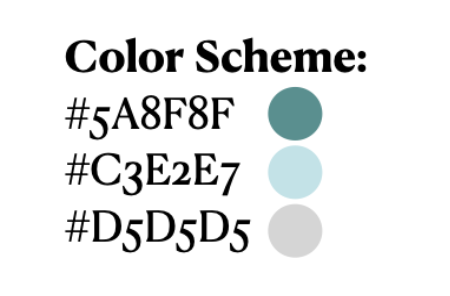
\includegraphics[width=0.2\linewidth]{thesis//chapters//images/colorScheme.png}
    \caption{Color Scheme}
    \label{fig:color-scheme}
\end{figure}

In addition, I aim to provide a design that is inclusive and accessible to all users. To achieve this, I carefully considered contrast and color choices, making sure they were tested against colorblind scales to ensure that the content is easily distinguishable and readable by a wide range of individuals.

To add a friendly and inviting touch to the app, I incorporated images and graphics that resonate with a warm and approachable feel. These images are thoughtfully chosen to create a connection with users and enhance their engagement with the app, contributing to a positive and enjoyable user experience.

In the following sections, you will see my initial prototype designs.

\section{Onboarding View}

The onboarding view consists of screens designed to introduce users to the app's key features and benefits. This view is essential for guiding new users and helping them get acquainted with the platform. The screens are simplistic and visually appealing, setting a positive tone for the user's journey.

The Set Up form asks the user to input key information, such as their name, birthdate, and allergens, and asks the user if they will allow the application to share data with Apple Health. This is a crucial step in the onboarding process, as without allowing access, the user will not have access to key insights and a tailored app experience.

\begin{figure}[H]
    \centering
    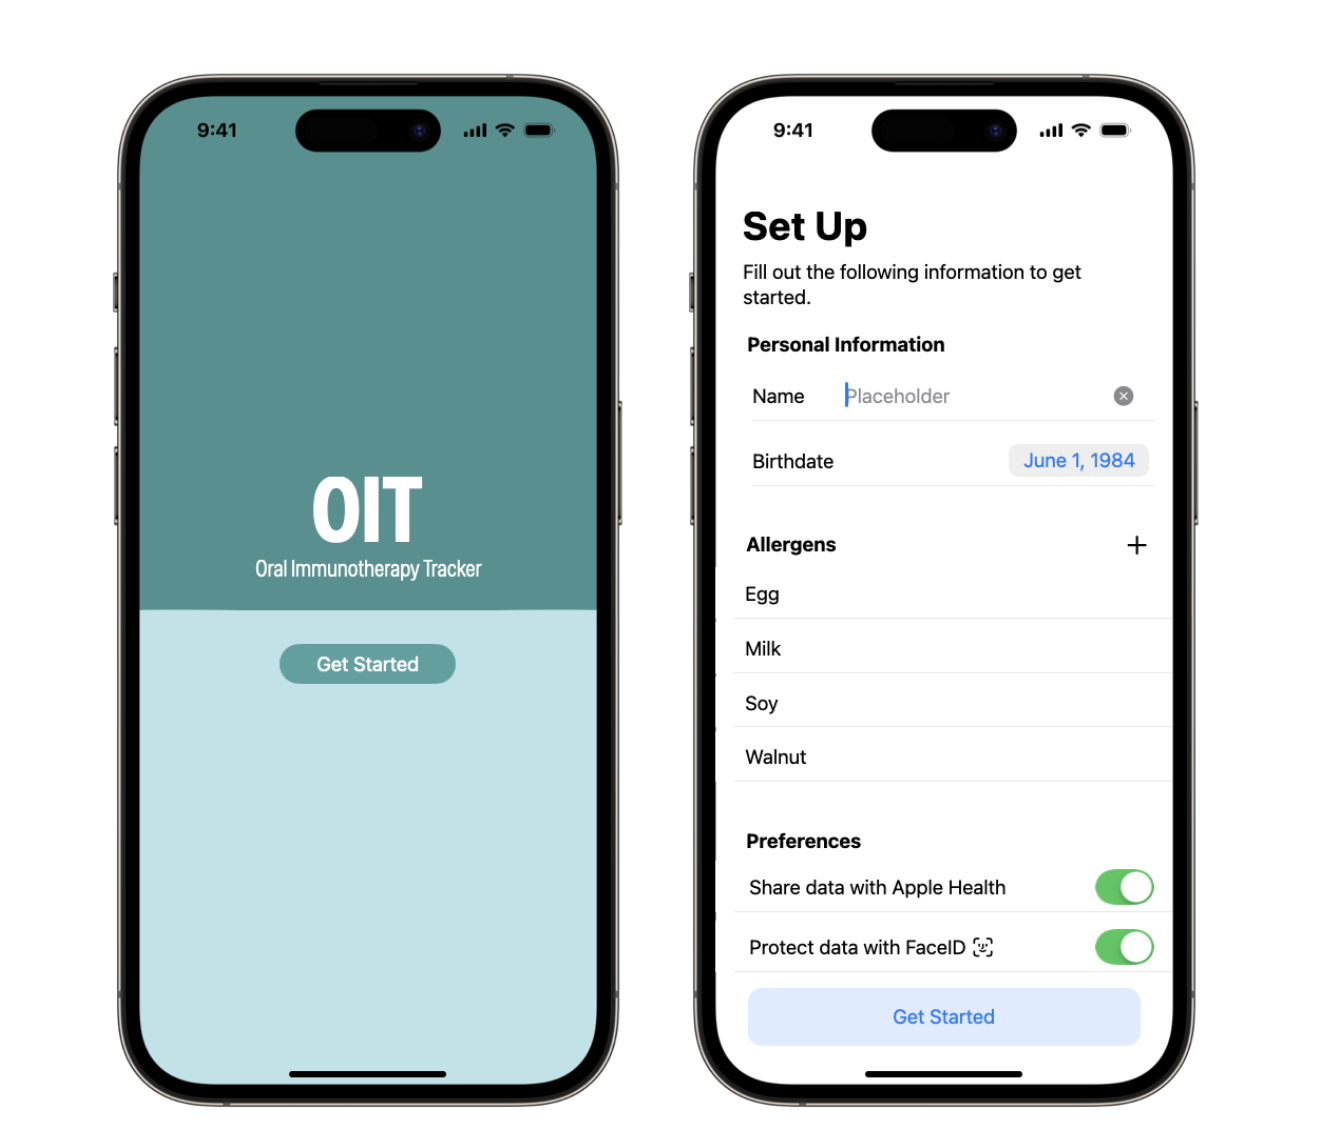
\includegraphics[width=0.7\linewidth]{thesis//chapters//images/onboarding-screens.png}
    \caption{Onboarding Screens}
    \label{fig:onboarding-screens}
\end{figure}

\section{Today Tab}

The Today Tab serves as the core of the app, where users view and log dose and symptom information for the selected date. The design prioritizes clarity and easy navigation, ensuring that users can quickly find the information they need. A sliding weekly calendar view allows the user to select a date, or the month button in the top right corner allows the user to switch to a monthly view. 

\begin{figure}[H]
    \centering
    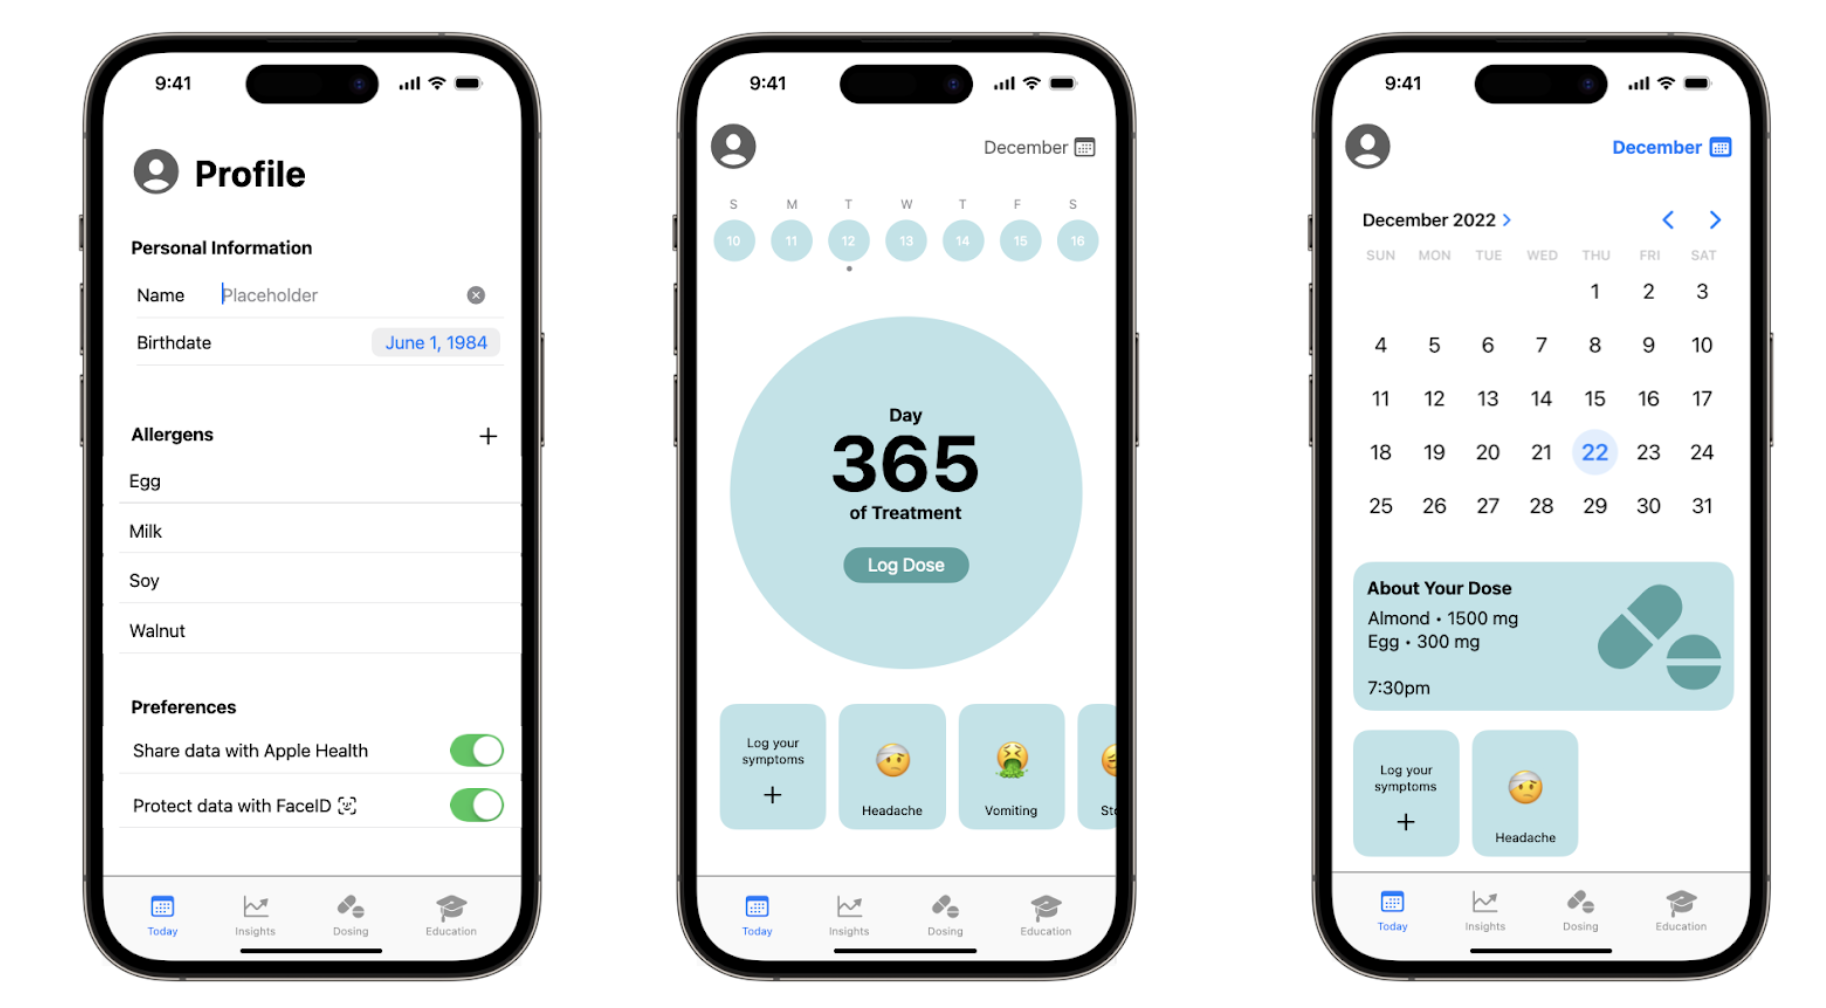
\includegraphics[width=1\linewidth]{thesis//chapters//images/todayTabScreens.png}
    \caption{Today Tab Screens}
    \label{fig:today-tab-screens}
\end{figure}

\section{Dose and Symptom Pop-Ups}

The dose and symptom pop-ups are opened when the user goes to log a dose or symptom in the Today tab. These pop-ups are designed to be user-friendly, with helpful graphics, and to make it take minimal time to log a dose or symptom.

\begin{figure}[H]
    \centering
    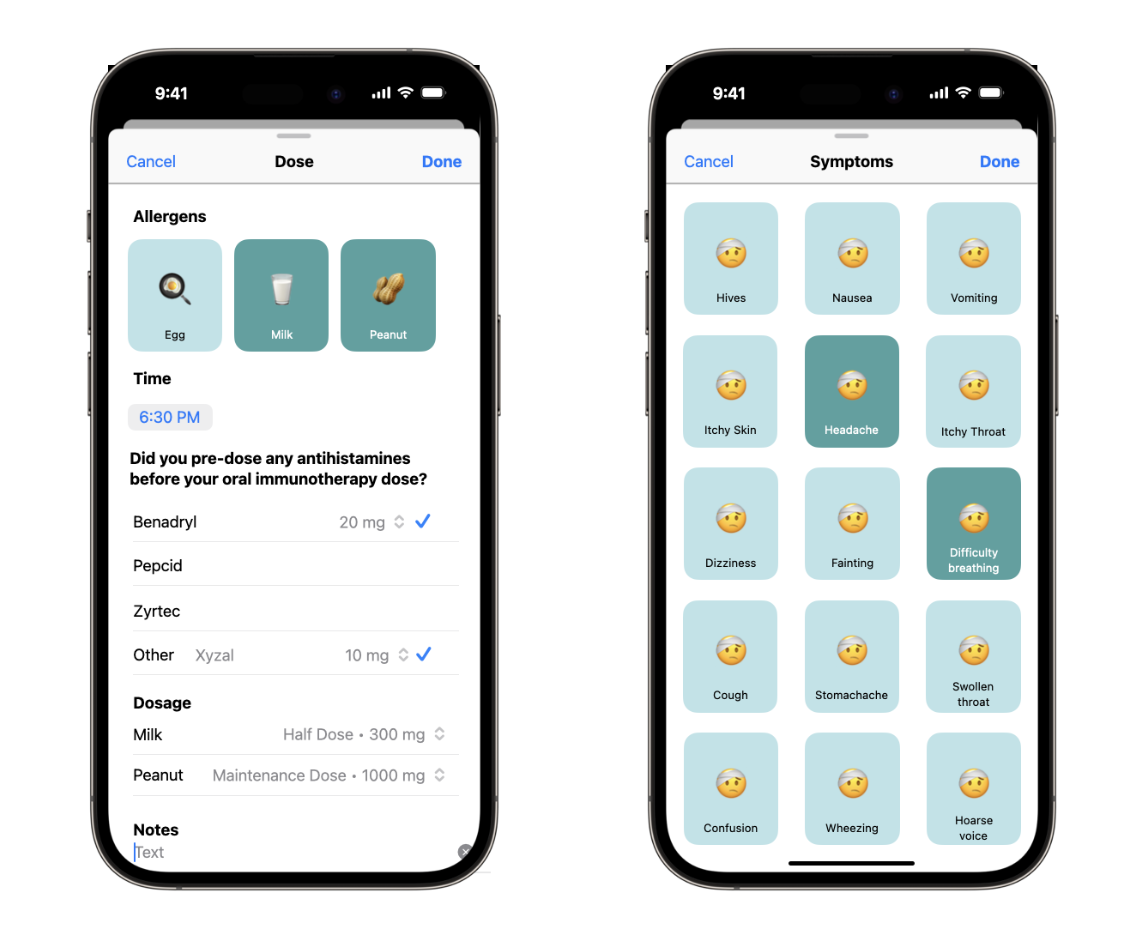
\includegraphics[width=0.7\linewidth]{thesis//chapters//images/doseAndSymptomPopUps.png}
    \caption{Dose and Symptoms Pop-Ups}
    \label{fig:dose-and-symptom-pop-ups}
\end{figure}

\section{Insights Tab}

\begin{figure}[H]
    \centering
    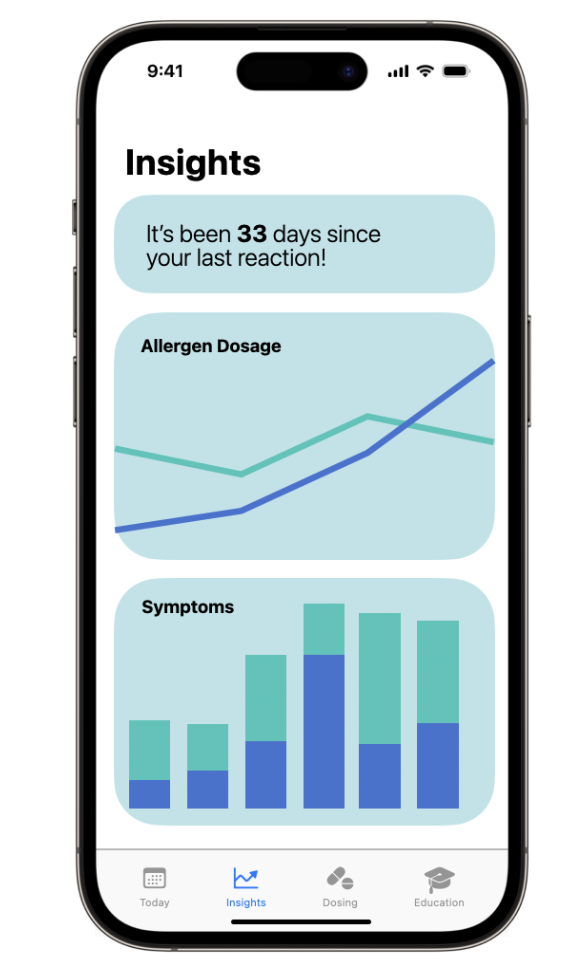
\includegraphics[width=0.3\linewidth]{thesis//chapters//images/insightsTab.png}
    \caption{Insights Tab}
    \label{fig:insights-tab}
\end{figure}

\section{Dosing Tab}

The dosing tab

\begin{figure}[H]
    \centering
    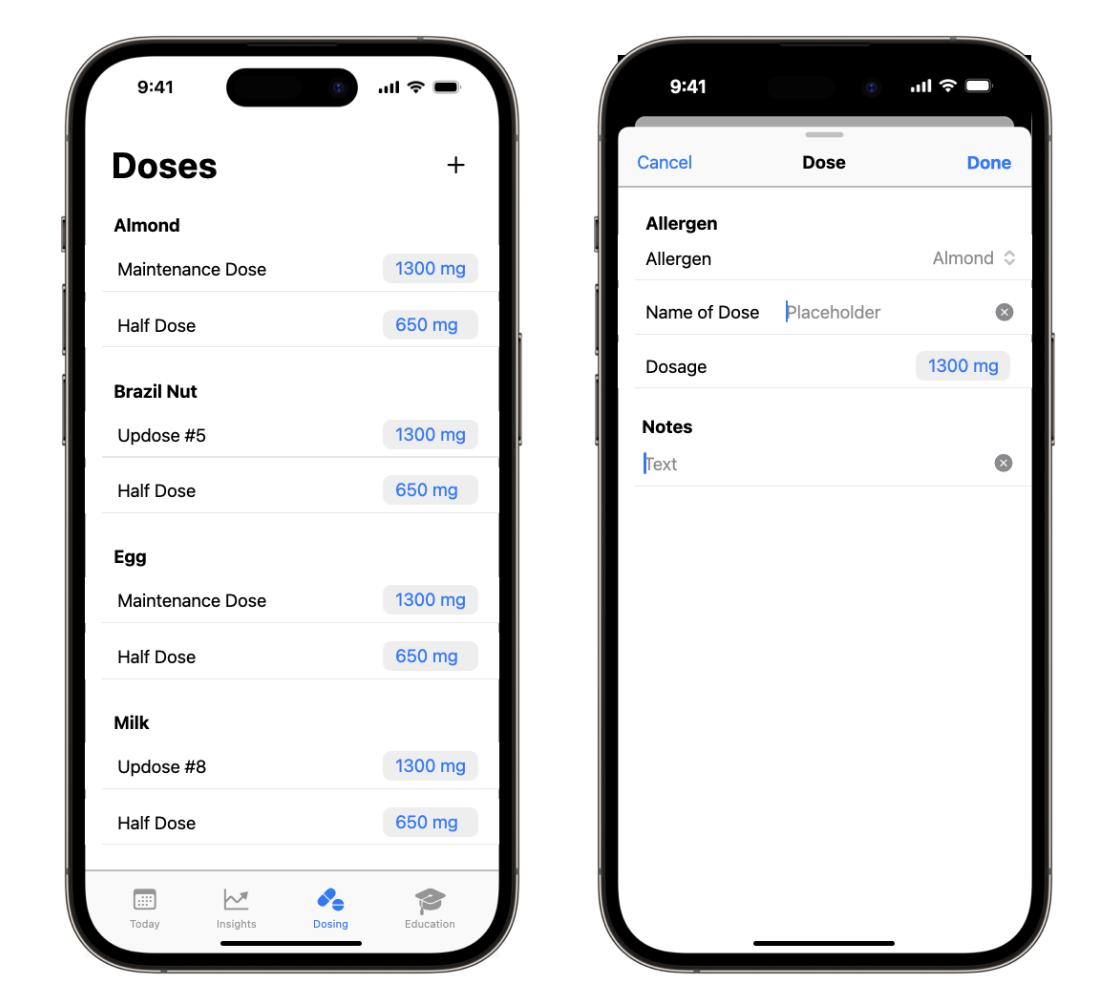
\includegraphics[width=0.7\linewidth]{thesis//chapters//images/dosingTabScreens.png}
    \caption{Dosing Tab Screens}
    \label{fig:dosing-tab}
\end{figure}

\section{Education Tab}

\begin{figure}[H]
    \centering
    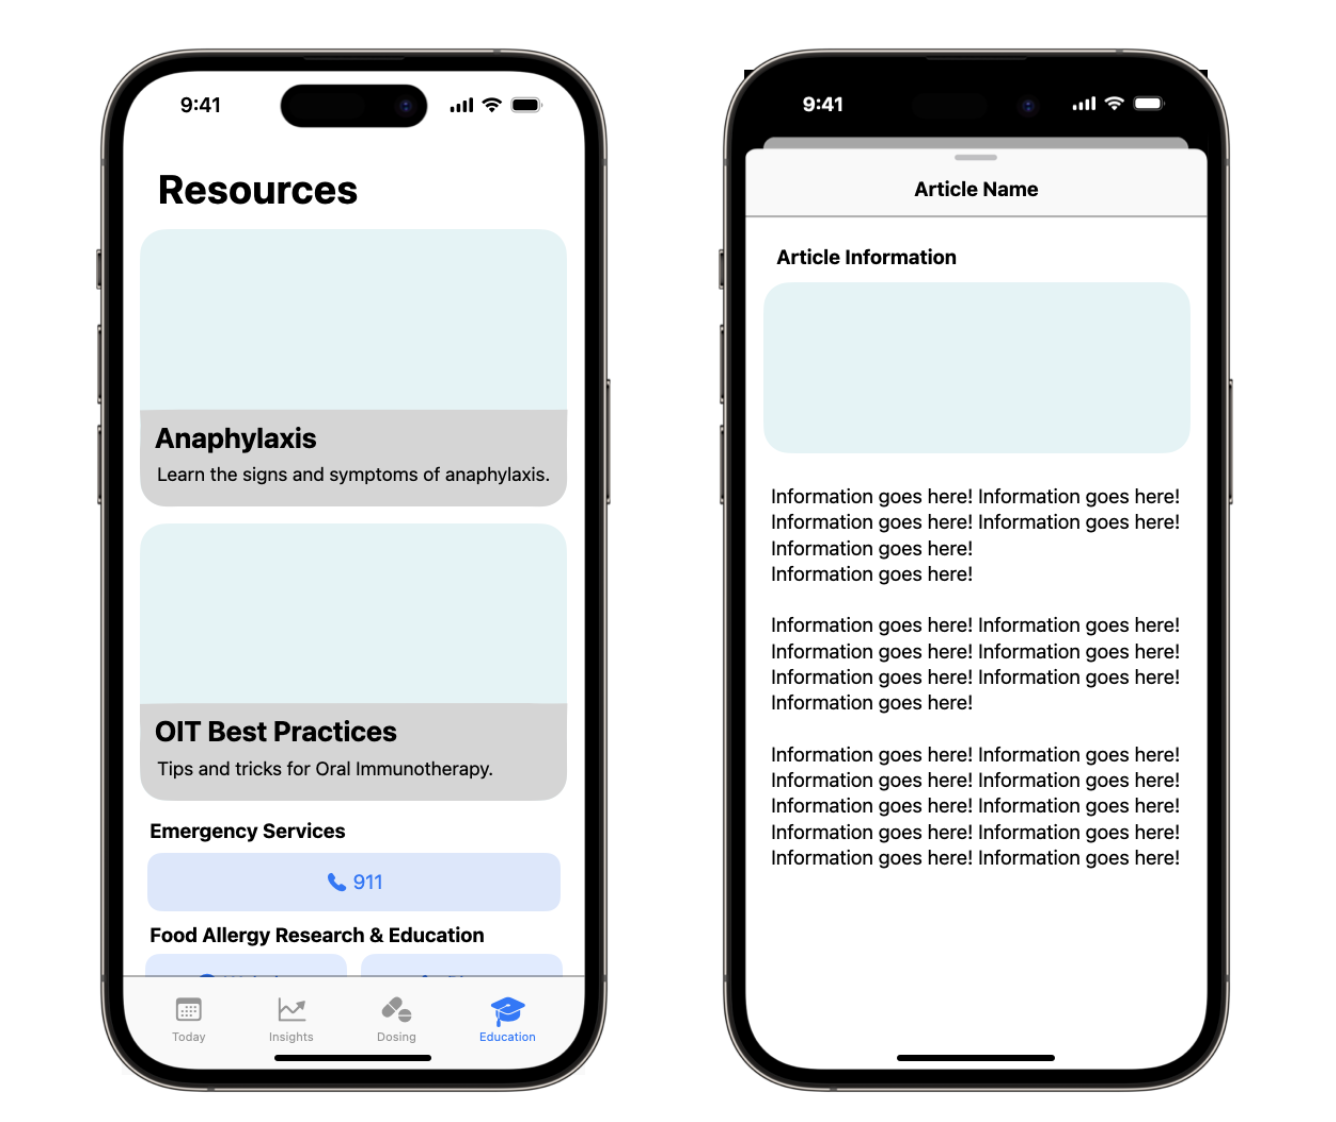
\includegraphics[width=0.7\linewidth]{thesis//chapters//images/education-tab-screens.png}
    \caption{Education Tab Screens}
    \label{fig:education-tab}
\end{figure}


\chapter{Software Design}

\section{General Architecture}

My application will be written in Swift and SwiftUI. The file architecture diagram in Figure \ref{fig:overall-file-architecture} serves as the foundational blueprint for my application. This visual representation offers a high-level overview of how data and functionalities are organized within the application. It outlines the structure of the app, showcasing the relationships between various components, data storage, and user interfaces. The teal files represent UI-level views, whereas the grey files represent classes that are at a lower level.

\begin{figure}[H]
    \centering
    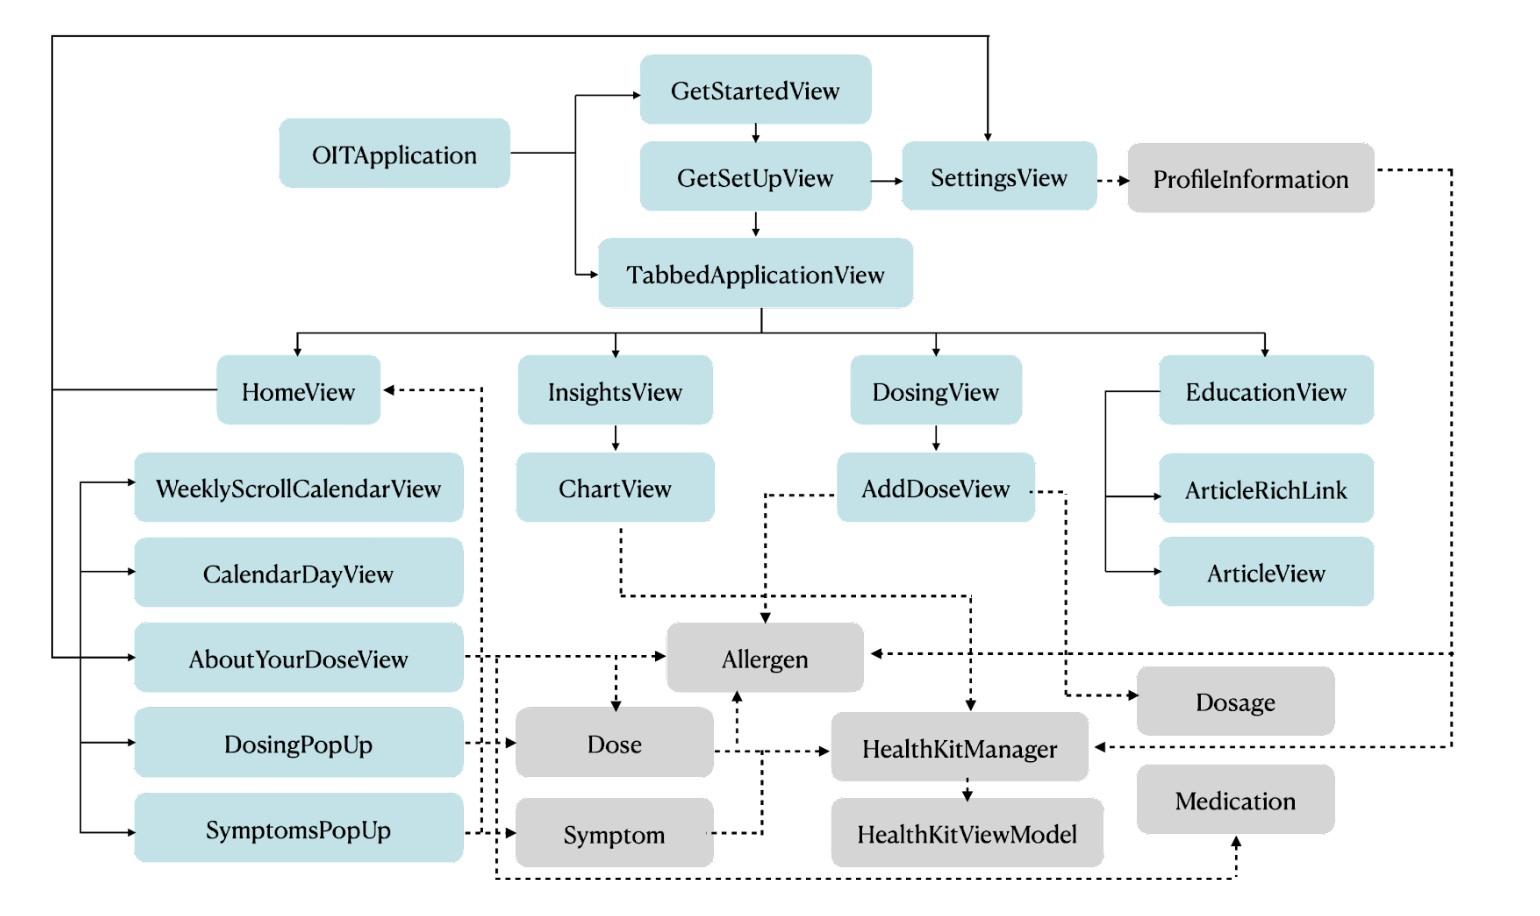
\includegraphics[width=1\linewidth]{thesis/chapters/images/overallFileArchitecture.png}
    \caption{Overall File Architecture}
    \label{fig:overall-file-architecture}
\end{figure}

\section{APIs}

Leveraging a combination of powerful APIs, my application aims to provide an enhanced and user-centric healthcare experience. I plan to utilize HealthKit, an integral component of the iOS ecosystem, which acts as a central repository for health and fitness data. With the user's explicit consent, my application will seamlessly integrate with HealthKit, facilitating the access and sharing of vital health information from the user's iPhone and Apple Watch \cite{HealthKit}. This integration will not only enable the application to provide personalized insights but also enhance the accuracy and reliability of the data we collect.

In addition, CareKit stands as another essential pillar in my app's framework. CareKit empowers users to take control of their health, enabling us to offer functionalities that support trend analysis, goal setting, and incentives. With CareKit 2.0's availability for iOS 13 and iPadOS 13 and above, my app will be able to provide a comprehensive health management experience, fostering a proactive approach to Oral Immunotherapy \cite{CareKit}.

To transform data into informative visualizations and offer a visually appealing user interface, I plan to implement the Swift Charts framework. Swift Charts offers a concise SwiftUI-based solution for creating a wide array of customizable charts \cite{SwiftCharts}. This powerful tool provides a range of essential building blocks, such as marks, scales, axes, and legends, which I can creatively combine to develop interactive and data-driven charts. These visualizations will not only enhance the user's understanding of their OIT journey but also make the app more engaging and informative.

Lastly, Swift Data will play a pivotal role in ensuring data persistence and accessibility across app launches. This framework simplifies the management of custom data types, making it easier to store and retrieve information efficiently \cite{SwiftData}. By integrating Swift Data with SwiftUI, I can seamlessly fetch and display key data, creating a seamless and reliable user experience. Whether it's preserving user progress or maintaining essential healthcare records, Swift Data will be instrumental in maintaining data integrity and availability.

By harnessing the capabilities of HealthKit, CareKit, Swift Charts, and Swift Data, I aim to deliver a comprehensive, informative, and user-friendly platform for individuals undergoing oral immunotherapy, transforming the way they manage their health and improve their overall well-being.

\section{Class diagrams}

The Class Diagrams below serve as a blueprint for the software development of the application. By visually representing classes and their attributes, this section delves into the heart of the application's design. Following UML standards, each diagram shows the private and public variables and methods for the class.

\begin{table}[ht]
\centering
\caption{Class Diagram: OITApplication}

\hspace{1em}
\renewcommand{\arraystretch}{1.7}

\begin{tabular}{|l|}
\hline
\textbf{OITApplication} \\
\hline
– hasAppBeenOpenedBefore: Bool \\
\hline
\end{tabular}
\end{table}

\begin{table}[H]
\centering
\caption{Class Diagram: TabbedApplicationView}

\hspace{1em}
\renewcommand{\arraystretch}{1.7}

\begin{tabular}{|l|}
\hline
\textbf{TabbedApplicationView} \\
\hline
– homeViewTab: NavigationView \\
– insightsViewTab: NavigationView \\
– dosingViewTab: NavigationView \\
– educationViewTab: NavigationView \\
\hline
\end{tabular}
\end{table}

\begin{table}[H]
\centering
\caption{Class Diagram: GetStartedView}

\hspace{1em}
\renewcommand{\arraystretch}{1.7}

\begin{tabular}{|l|}
\hline
\textbf{GetStartedView} \\
\hline
– getStartedButton: Button \\
– appTitle: Text \\
– backgroundColor: Color \\
\hline
\end{tabular}
\end{table}

\begin{table}[H]
\centering
\caption{Class Diagram: GetSetUpView}

\hspace{1em}
\renewcommand{\arraystretch}{1.7}

\begin{tabular}{|l|}
\hline
\textbf{GetSetUpView} \\
\hline
– title: String \\
+ personalInformation: ProfileInformation \\
– settingsView: SettingsView \\
– getStartedButton: Button \\
\hline
\end{tabular}
\end{table}

\begin{table}[H]
\centering
\caption{Class Diagram: ProfileInformation}

\hspace{1em}
\renewcommand{\arraystretch}{1.7}

\begin{tabular}{|l|}
\hline
\textbf{ProfileInformation} \\
\hline
+ name: String \\
+ birthdate: Date \\
+ allergens: [Allergen] \\
+ shareDataWithAppleHealth: Bool \\
+ protectDataWithFaceID: Bool \\
\hline
\end{tabular}
\end{table}

\begin{table}[H]
\centering
\caption{Class Diagram: Allergen}

\hspace{1em}
\renewcommand{\arraystretch}{1.7}

\begin{tabular}{|l|}
\hline
\textbf{Allergen} \\
\hline
– AllergenType: enumeration(String) \\
+ allergen: AllergenType \\
\hline
\end{tabular}
\end{table}

\begin{table}[H]
\centering
\caption{Class Diagram: Symptom}

\hspace{1em}
\renewcommand{\arraystretch}{1.7}

\begin{tabular}{|l|}
\hline
\textbf{Symptom} \\
\hline
– SymptomType: enumeration(HKCategoryType) \\
+ symptom: HKCategoryType \\
\hdashline
+ getSymptomString( ): String \\
\hline
\end{tabular}
\end{table}

\begin{table}[ht]
\centering
\caption{Class Diagram: Medication}

\hspace{1em}
\renewcommand{\arraystretch}{1.7}

\begin{tabular}{|l|}
\hline
\textbf{Medication} \\
\hline
– MedicationType: enumeration(HKClinicalTypeIdentifier) \\
+ medication: HKClinicalTypeIdentifier \\
\hdashline
+ getMedicationString( ): String \\
\hline
\end{tabular}
\end{table}

\begin{table}[H]
\centering
\caption{Class Diagram: SymptomsPopUp}

\hspace{1em}
\renewcommand{\arraystretch}{1.7}

\begin{tabular}{|l|}
\hline
\textbf{SymptomsPopUp} \\
\hline
+ symptomsSelected: [Symptom] \\
- symptomsButtons: [Button] \\
\hdashline
– changeButtonAppearance( ): Void \\
\hline
\end{tabular}
\end{table}

\begin{table}[H]
\centering
\caption{Class Diagram: HomeView}

\hspace{1em}
\renewcommand{\arraystretch}{1.7}

\begin{tabular}{|l|}
\hline
\textbf{HomeView} \\
\hline
– todayDate: Date \\
+ selectedDate: Date \\
– weekView: Bool \\
– logSymptoms: Bool \\
– logDose: Bool \\
– profileButton: Button \\
– calendarButton: Button \\
– weeklyScrollCalendarView: WeeklyScrollCalendarView \\
– logDoseButton: Button \\
– logSymptomsButton: Button \\
– aboutYourDoseView: AboutYourDoseView \\
– dose: Dose \\
– symptoms: Symptoms \\
\hline
\end{tabular}
\end{table}

\begin{table}[H]
\centering
\caption{Class Diagram: WeeklyScrollCalendarView}

\hspace{1em}
\renewcommand{\arraystretch}{1.7}

\begin{tabular}{|l|}
\hline
\textbf{WeeklyScrollCalendarView} \\
\hline
– scrollView: ScrollView \\
– dayCircle: CalendarDayView \\
\hdashline
+ startOfWeek( ): Date \\
+ monthHeader( ): String \\
\hline
\end{tabular}
\end{table}

\begin{table}[ht]
\centering
\caption{Class Diagram: CalendarDayView}

\hspace{1em}
\renewcommand{\arraystretch}{1.7}

\begin{tabular}{|l|}
\hline
\textbf{CalendarDayView} \\
\hline
– date: Date \\
– isSelected: Bool \\
– dayText: Text \\
– dateText: Text \\
\hdashline
+ getDayText( ): String \\
+ getDateText( ): String \\
\hline
\end{tabular}
\end{table}

\begin{table}[H]
\centering
\caption{Class Diagram: AboutYourDoseView}

\hspace{1em}
\renewcommand{\arraystretch}{1.7}

\begin{tabular}{|l|}
\hline
\textbf{AboutYourDoseView} \\
\hline
– titleText: Text \\
– allergenText: Text \\
– timeOfDose: Date \\
– dose: Dose \\
– doseIcon: Image \\
\hline
\end{tabular}
\end{table}

\begin{table}[ht]
\centering
\caption{Class Diagram: Dose}

\hspace{1em}
\renewcommand{\arraystretch}{1.7}

\begin{tabular}{|l|}
\hline
\textbf{Dose} \\
\hline
+ name: String \\
+ allergens: [Allergen] \\
+ dosages: [[Allergen, float]] \\
+ dateOfDose: Date \\
+ timeOfDose: Date \\
+ preDoseMedications: [Medication] \\
+ notes: String \\
\hline
\end{tabular}
\end{table}

\begin{table}[H]
\centering
\caption{Class Diagram: DosingPopUp}

\hspace{1em}
\renewcommand{\arraystretch}{1.7}

\begin{tabular}{|l|}
\hline
\textbf{DosingPopUp} \\
\hline
+ dose: Dose \\
– allergenButtons: [Button] \\
– saveDoseButton: Button \\
\hdashline
– saveDose( ): Void \\
\hline
\end{tabular}
\end{table}

\begin{table}[H]
\centering
\caption{Class Diagram: SettingsView}

\hspace{1em}
\renewcommand{\arraystretch}{1.7}

\begin{tabular}{|l|}
\hline
\textbf{SettingsView} \\
\hline
+ personalInformation: ProfileInformation \\
- nameTextField: TextField \\
- birthdateDatePicker: DatePicker \\
- addAllergenButton: Button \\
- shareDataWithAppleHealth: Toggle \\
- enableFaceID: Toggle \\
\hline
\end{tabular}
\end{table}

\begin{table}[H]
\centering
\caption{Class Diagram: HealthKitManager}

\hspace{1em}
\renewcommand{\arraystretch}{1.7}

\begin{tabular}{|l|}
\hline
\textbf{HealthKitManager} \\
\hline
+ symptoms: [HKCategoryType] \\
– dataToRead: [HKCategoryType] \\
– dataToWrite: [HategoryType] \\
\hdashline
+ setUpHealthRequest() \\
\hline
\end{tabular}
\end{table}

\begin{table}[H]
\centering
\caption{Class Diagram: HealthKitViewModel}

\hspace{1em}
\renewcommand{\arraystretch}{1.7}

\begin{tabular}{|l|}
\hline
\textbf{HealthKitViewModel} \\
\hline
+ healthStore: HKHealthStore \\
+ healthKitManager: HKManager \\
+ isAuthorized: Bool \\
\hdashline
+ healthRequest() \\
+ changeAuthorizationStatus() \\
\hline
\end{tabular}
\end{table}

\begin{table}[H]
\centering
\caption{Class Diagram: InsightsView}

\hspace{1em}
\renewcommand{\arraystretch}{1.7}

\begin{tabular}{|l|}
\hline
\textbf{InsightsView} \\
\hline
– title: Text \\
- charts: [ChartView] \\
\hline
\end{tabular}
\end{table}

\begin{table}[H]
\centering
\caption{Class Diagram: ChartView}

\hspace{1em}
\renewcommand{\arraystretch}{1.7}

\begin{tabular}{|l|}
\hline
\textbf{ChartView} \\
\hline
– chartType: Chart \\
– chartData: [AnyObject] \\
\hline
\end{tabular}
\end{table}

\begin{table}[H]
\centering
\caption{Class Diagram: DosingView}

\hspace{1em}
\renewcommand{\arraystretch}{1.7}

\begin{tabular}{|l|}
\hline
\textbf{DosingView} \\
\hline
- title: Text \\
– addNewDoseButton: Button \\
+ allergensAndDoses: [Allergen, [Dosage]] \\
- tableView: TableView \\
\hline
\end{tabular}
\end{table}

\begin{table}[H]
\centering
\caption{Class Diagram: AddDoseView}

\hspace{1em}
\renewcommand{\arraystretch}{1.7}

\begin{tabular}{|l|}
\hline
\textbf{AddDoseView} \\
\hline
– allergen: Picker \\
– nameOfDose: TextField \\
– dosage: TextField \\
– notes: TextField \\
– saveDosageButton: Button \\
+ savedDosage: Dosage \\
\hline
\end{tabular}
\end{table}

\begin{table}[H]
\centering
\caption{Class Diagram: Dosage}

\hspace{1em}
\renewcommand{\arraystretch}{1.7}

\begin{tabular}{|l|}
\hline
\textbf{Dosage} \\
\hline
+ allergen: Allergen \\
+ nameOfDose: String \\
+ dosage: Int \\
+ notes: String \\
\hline
\end{tabular}
\end{table}

\begin{table}[H]
\centering
\caption{Class Diagram: EducationView}

\hspace{1em}
\renewcommand{\arraystretch}{1.7}

\begin{tabular}{|l|}
\hline
\textbf{EducationView} \\
\hline
- title: Text \\
– articles: [ArticleRichLink] \\
- resourceHeadings: [String] \\
- resourceButtons: [Button] \\
\hline
\end{tabular}
\end{table}

\begin{table}[H]
\centering
\caption{Class Diagram: ArticleRichLink}

\hspace{1em}
\renewcommand{\arraystretch}{1.7}

\begin{tabular}{|l|}
\hline
\textbf{ArticleRichLink} \\
\hline
– title: Text \\
– description: Text \\
– image: Image \\
– article: ArticleView \\
\hline
\end{tabular}
\end{table}

\begin{table}[H]
\centering
\caption{Class Diagram: ArticleView}

\hspace{1em}
\renewcommand{\arraystretch}{1.7}

\begin{tabular}{|l|}
\hline
\textbf{ArticleView} \\
\hline
– title: Text \\
– description: Text \\
– image: Image \\
– articleInformation: Text \\
\hline
\end{tabular}
\end{table}


\chapter{Constraints and Standards}

Before diving into the development process, it is important to recognize and address the various constraints and standards that shape and govern the project, so that I can plan for them. This section delves into the constraints that have influenced the project's trajectory, ranging from time limitations imposed by academic schedules to legal considerations in ensuring the utmost user privacy. Simultaneously, the section explores the standards adhered to throughout the development process, aligning the project with recognized benchmarks in software engineering, accessibility, and interoperability. By understanding and adhering to these constraints and standards, my application will not only fit within the confines of practical realities but also conform to industry best practices, fostering a robust and ethically sound healthcare solution.

\section{Constraints}

Developing a software application as a solo endeavor brings its own set of challenges, and recognizing and navigating these constraints is paramount for success. While financial considerations are mitigated in this context, time and legal factors emerge as critical constraints that demand careful attention.

\begin{itemize}
    \item \textbf{Time:} The timeline of the senior capstone experience and academic deadlines impose significant time constraints on all phases of the project. Structuring the project plan and development process within these allocated timeframes is essential for meeting deliverables and achieving project goals.
    \item \textbf{Legal:} Legal considerations, particularly healthcare privacy regulations such as HIPAA, stand as significant factors influencing the project. Ensuring strict compliance with these regulations is non-negotiable to safeguard patient data and uphold legal standards. This legal awareness adds complexity to the development process, demanding meticulous attention to detail.
    \item \textbf{Maintenance Considerations:} Planning for the long-term maintenance of the project post-deployment is a critical aspect of the development process. Designing the system with foresight for future updates and enhancements ensures that ongoing maintenance can be executed seamlessly. This forward-thinking approach aims to maximize the application's lifespan and adaptability, addressing potential challenges before they arise.
\end{itemize}

In navigating these constraints, a strategic allocation of resources and a proactive approach to time management will be key to the success of the project. By addressing these challenges head-on, I hope to lay the foundation for a robust and sustainable software solution.

\section{Standards}

Ensuring that the developed application aligns with established industry standards is paramount for creating a robust, reliable, and inclusive healthcare solution. The adherence to specific standards across various facets of the project speaks to a commitment to excellence and user-centric design.

\begin{itemize}
    \item \textbf{Unified Modeling Language (UML) Standards}: Unified Modeling Language (UML) Standards constitute a crucial framework for expressing and communicating the structural and behavioral aspects of a software system in a standardized visual notation. UML provides a common language for software developers, analysts, and designers to collaboratively conceptualize, design, and document complex systems. These standards encompass a variety of diagram types, including class diagrams, sequence diagrams, and use case diagrams, each serving a distinct purpose in capturing different facets of system architecture and functionality \cite{UML}. In creating my diagrams and plans for this project, I've utilized UML standards, ensuring ease of readability in the software engineering community.
    \item \textbf{IEEE Standards:} Adhering to a suite of IEEE standards has been integral to the development process. Particularly, in the realm of software engineering practices, these standards have acted as guiding principles \cite{IEEEStd}. I've outlined some of the IEEE standards I've followed below:
        \begin{itemize}
        \item \textbf{IEEE 830 - Software Requirements Specification:}
        This standard provides guidelines for preparing a software requirements specification document, ensuring clarity and completeness in documenting the functional and non-functional requirements of the software \cite{IEEE830}.
        \item \textbf{IEEE 1016 - Software Design Descriptions:}
        This standard outlines the structure and content of software design descriptions, aiding in the effective communication of design details among project stakeholders \cite{IEEE1016}.
        \item \textbf{IEEE 1471 - Architecture Description:}
        Focused on architectural descriptions, this standard offers guidance on documenting and presenting system architectures, helping to ensure consistency and comprehensibility \cite{IEEE1471}.
        \item \textbf{IEEE 830.1 - Recommended Practice for Software Requirements Specifications Extensions:}
        This standard offers additional guidance on extending and customizing IEEE 830 for specific project needs, potentially useful in tailoring requirements specifications \cite{IEEE830.1}.
        \end{itemize}
    \item \textbf{ISO Standards:} The application also adheres to ISO standards, encompassing programming languages and design methodologies, some of which are listed below \cite{ISO}.
        \begin{itemize}
        \item \textbf{ISO/IEC 9126 - Software Engineering - Product Quality:} This standard provides a framework for defining and evaluating software quality characteristics, including functionality, reliability, usability, efficiency, maintainability, and portability \cite{ISO9126}.
        \item \textbf{ISO/IEC 25000 - Systems and software engineering - Systems and software Quality Requirements and Evaluation (SQuaRE):} This series of standards provides guidance on the application of the ISO/IEC 9126 quality model and defines a set of quality requirements and evaluation standards for software products \cite{ISO25000}.
        \item \textbf{ISO 9241-171:} This ISO standard provides guidelines for designing software that is accessible to people with disabilities. It covers aspects like visual, auditory, and cognitive accessibility \cite{ISO9241-171}.
        \end{itemize}
    \item \textbf{Apple Standards}: Because I am creating an iPhone application, it is important to follow the Apple-specific standards listed below.
        \begin{itemize}
            \item \textbf{Human Interface Guidelines (HIG):} Apple's HIG provides design principles and recommendations for creating a consistent and intuitive user experience across iOS, macOS, watchOS, and tvOS. When designing the UI of my application, I closely followed the HIG \cite{HIG}.
            \item \textbf{App Store Review Guidelines:} These guidelines outline the criteria that apps must meet to be accepted on the App Store. It covers various aspects including app functionality, design, security, and more \cite{AppStore}.
            \item \textbf{Accessibility Guidelines:} Apple provides comprehensive accessibility guidelines for developers. This includes guidance on designing accessible user interfaces, providing alternative content for multimedia, and ensuring compatibility with VoiceOver, Apple's built-in screen reader \cite{AppleAccessibility}.
        \end{itemize}
    \item \textbf{Health Insurance Portability and Accountability Act (HIPAA) Compliance Standards:} HIPAA sets the standard for protecting sensitive patient data and defines how this information should be handled, stored, and transmitted \cite{HIPPA}.
    \begin{itemize}
        \item \textbf{Secure Data Transmission:} Ensure that all patient data transmitted between the application and any backend servers or databases is encrypted. HIPAA requires the use of secure communication protocols, such as TLS, to protect patient information during transmission.
        \item \textbf{Data Storage and Encryption:} Implement robust encryption mechanisms for stored patient data. This includes data at rest on servers or devices. Encryption helps safeguard patient information in the event of unauthorized access.
        \item \textbf{Access Controls:} Enforce strict access controls to limit who can access patient data within the application. Implement user authentication and authorization mechanisms to ensure that only authorized personnel can view or modify sensitive information.
    \end{itemize}
    
\end{itemize}
\chapter{Schedule}

This project requires a meticulously planned roadmap to navigate the complexities and milestones that lie ahead. The Gantt Chart in Figure \ref{fig:project-gantt-chart} serves as a visual compass, delineating the chronological sequence of tasks and deadlines essential for the successful completion of the project. Each bar, carefully plotted along the timeline, represents a crucial aspect of the thesis development process, offering a comprehensive overview of the project's progression. This dynamic tool not only aids in project management but also provides a clear visualization of interdependencies, helping to anticipate potential challenges and facilitating effective decision-making throughout the thesis endeavor.

\begin{figure} [H]
    \centering
    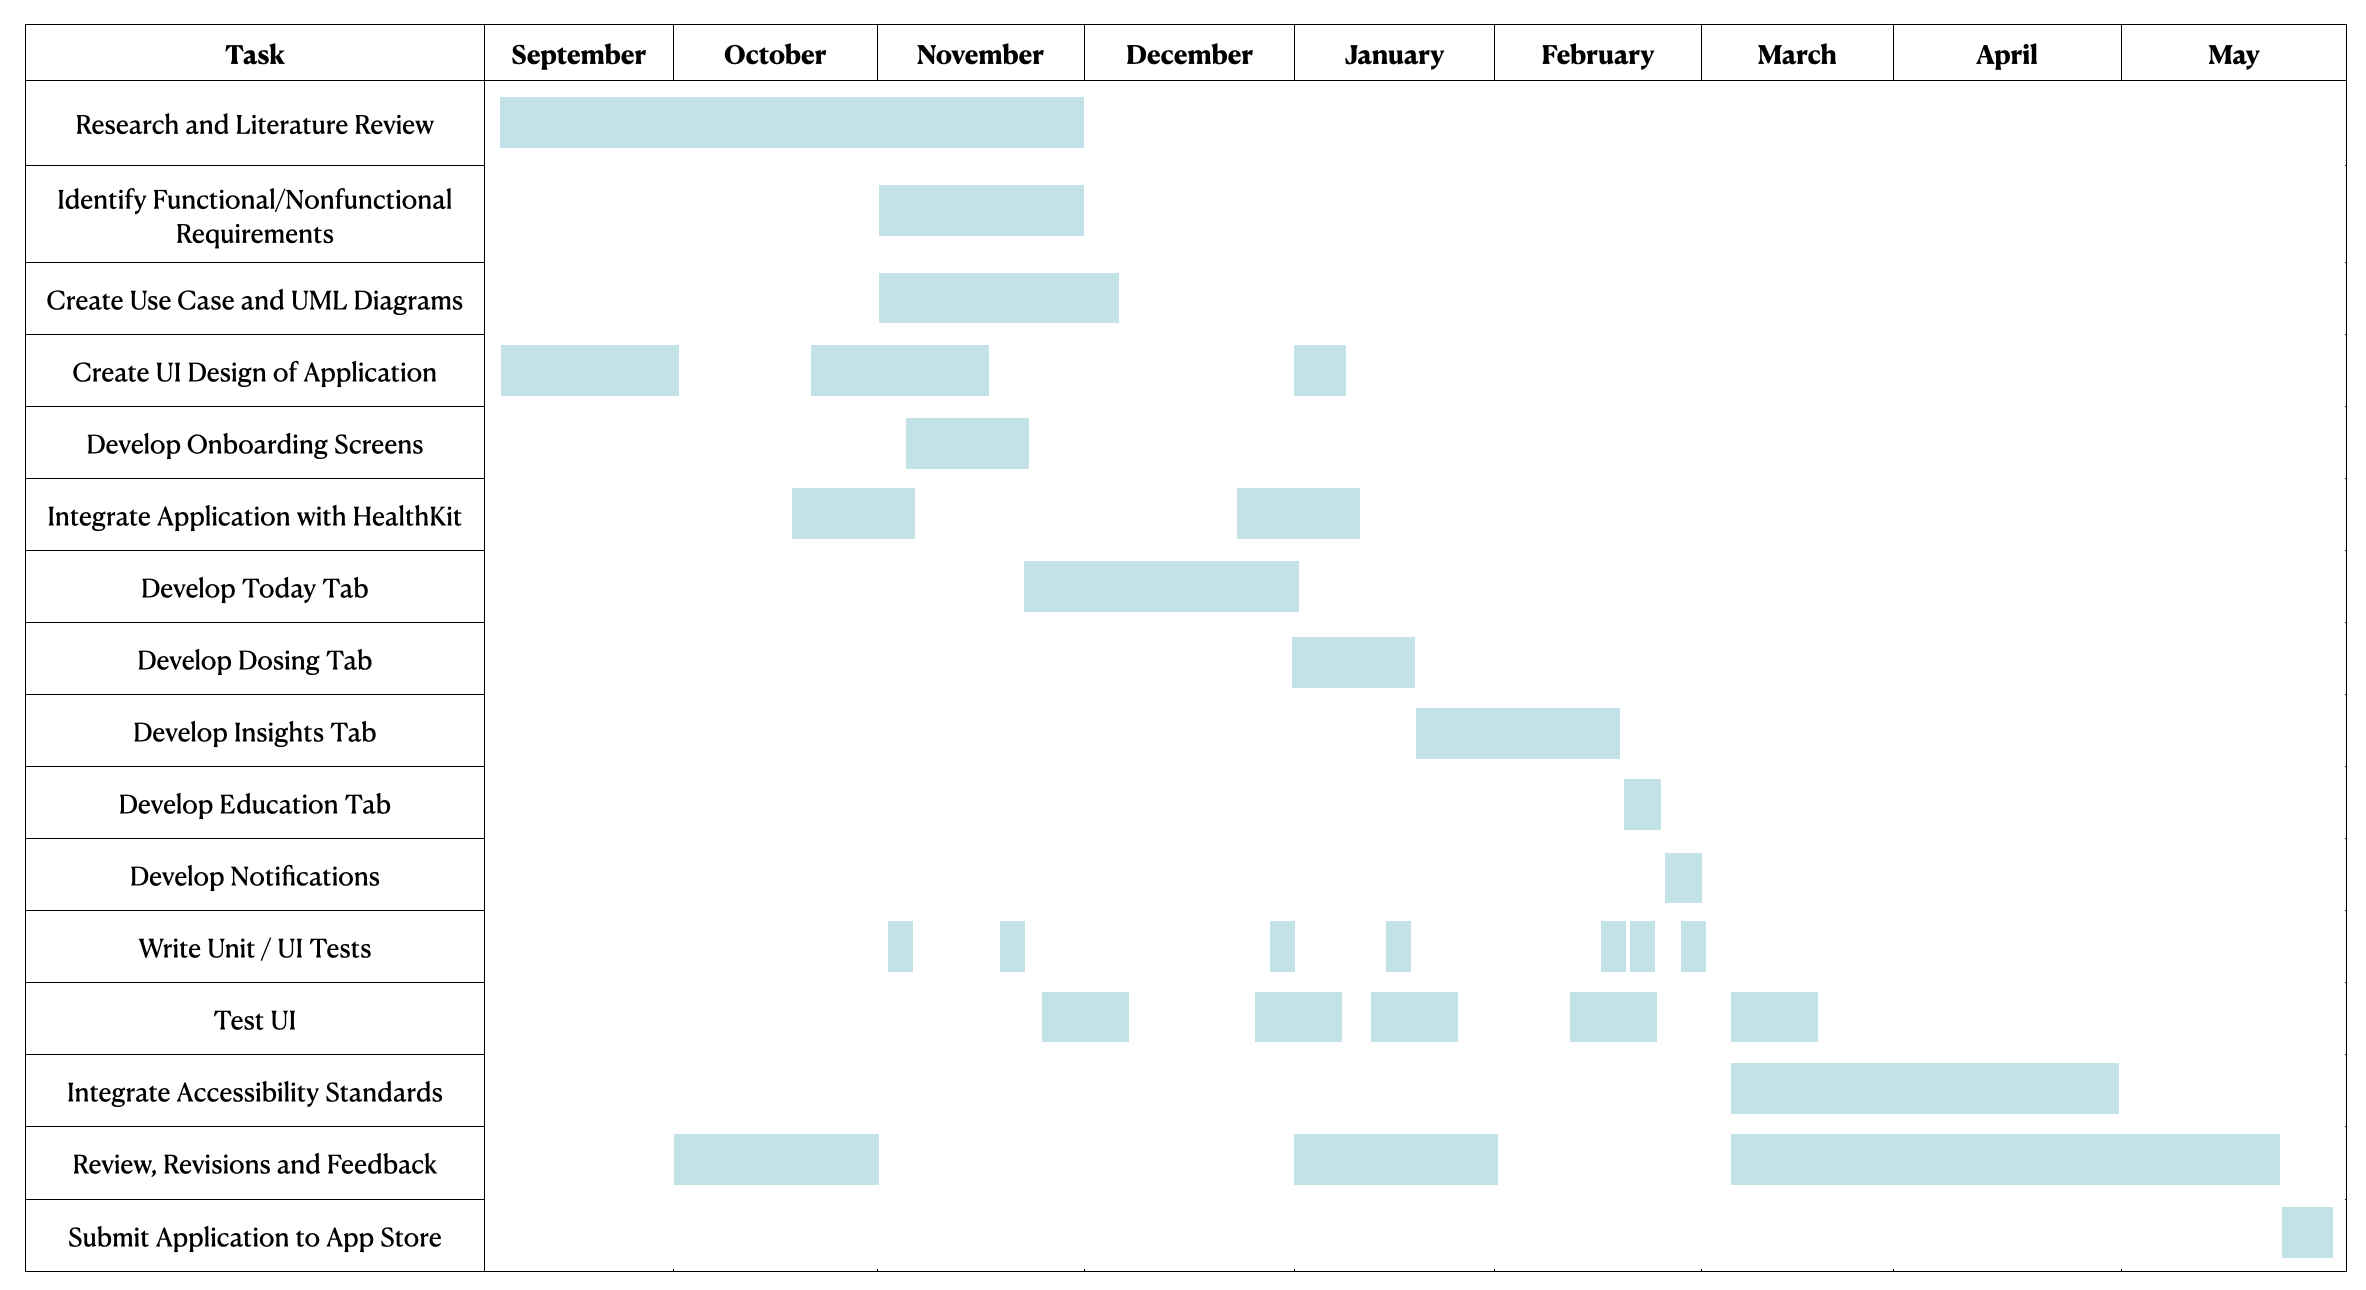
\includegraphics[width=1\linewidth]{thesis//chapters//images/ganttChart.png}
    \caption{Project Gantt Chart}
    \label{fig:project-gantt-chart}
\end{figure}


\chapter{Risk Analysis}

The development process is inherently complex, marked by uncertainties and challenges that have the potential to influence the successful completion of any project. In recognizing the dynamic nature of software development, it becomes crucial to proactively identify and analyze potential risks. This approach not only facilitates early detection but also enables the formulation of effective mitigation strategies to safeguard the project's trajectory.

Risk analysis is an indispensable component of project management, providing a structured framework for understanding, assessing, and addressing potential threats. It involves a systematic evaluation of uncertainties that could impact project objectives, timelines, and deliverables. By undertaking a comprehensive risk analysis, project teams can anticipate, prioritize, and respond to potential issues, minimizing the likelihood of disruptions and ensuring a smoother project progression.

The risk analysis table presented below serves as a strategic tool for capturing and categorizing risks that may manifest at various stages of the project lifecycle. Each entry in the table delineates a specific risk, accompanied by its probability of occurrence, severity, potential consequences, and recommended preventative measures. The probability is quantified on a scale from 0 to 1, severity is ranked from 1 to 10, and the impact is calculated as the product of probability and severity.

\begin{table} [H]
    \centering
    \hspace{1em}
    \renewcommand{\arraystretch}{1.5}
    \begin{tabular}{|p{10em}|c|c|c|p{10em}|p{10em}|}
        \hline
        \textbf{Risk} & \textbf{Probability} & \textbf{Severity} & \textbf{Impact} & \textbf{Consequences} & \textbf{Mitigation} \\
         \hline
         Constraints are not met & 0.5 & 8 & 4 & Application is incomplete & Consult with advisor for clarification, and check initial progress before proceeding \\
         \hline
         Unable to integrate with Apple HealthKit & 0.2 & 10 & 2 & User is unable to view their data in the Health app, or share data with their doctor & Research HealthKit, and abstract the HealthKit portion of the code, so that if this area isn't implemented, the app still works \\
         \hline
         Unable to implement feature(s) & 0.7 & 8 & 5.6 & Code is unfinished, or is finished, but with less features than originally planned & Ask for assistance to keep up with timeline, and prioritize tasks, so that lower priority items can be dropped if needed \\
         \hline
         App store policies are not met & 0.05 & 10 & 0.5 & Unable to submit the application to the App Store & Regularly check App Store policies, and update app criteria as needed \\
         \hline
         Application is not compatible with iPhone model & 0.1 & 10 & 1 & User is unable to use the application & Ensure that the APIs and technologies used have an appropriate minimum iOS, and that the code is tested on various iPhone models \\
         \hline
         Source control error & 0.4 & 4 & 1.6 & Setback in development, due to loss of work & Back up work in GitHub, and ensure code is pushed after major code changes \\
         \hline
         Not enough time & 0.5 & 7 & 3.5 & Unable to complete the project by the due date & Allow for more time than expected for development, and keep to the schedule defined in the previous chapter \\
         \hline
         Bugs & 1.0 & 4 & 4 & Subpar user experience, and implementation not working fully & Develop unit and UI tests as features are developed, and check functionality of each feature before continuing to the next \\
         \hline
         Developer unable to contribute & 0.2 & 10 & 2 & Progress on the project becomes stagnant, as there is only a single developer & Regularly check in with advisor on progress, and prioritize tasks, so that if the developer becomes indisposed for a period of time, lower priority items can be dropped \\
         \hline
    \end{tabular}
    \caption{Risk Analysis Table}
    \label{tab:risk_analysis}
\end{table}
\chapter{Implementation}


\chapter{Testing}

Testing is a pivotal component in the development lifecycle of the Oral Immunotherapy application, ensuring the reliability, functionality, and user experience align with the project goals. This chapter delves into the comprehensive testing strategies I employed throughout the project's development, encompassing Visual Testing, XCTests, and User Testing.

\section{Visual Testing}

Visual testing played a crucial role in ensuring the graphical elements and user interface (UI) components of the application met the desired standards. Leveraging Xcode's SwiftUI Canvas's previews, I systematically examined the visual representation of the app across different devices, screen sizes, phone orientations, and color schemes (e.g. light and dark modes). This approach allowed me to identify and rectify any layout inconsistencies, aesthetic issues, or UI element misalignments. 

In Figures \ref{fig:swiftUICanvas}, \ref{fig:swiftUICanvasColorVar}, \ref{fig:swiftUICanvasOrientationVar}, \ref{fig:swiftUICanvasDTVar}, and \ref{fig:deviceVar} you can see an example of the previews given in Xcode's SwiftUI Canvas.

\begin{figure} [H]
    \centering
    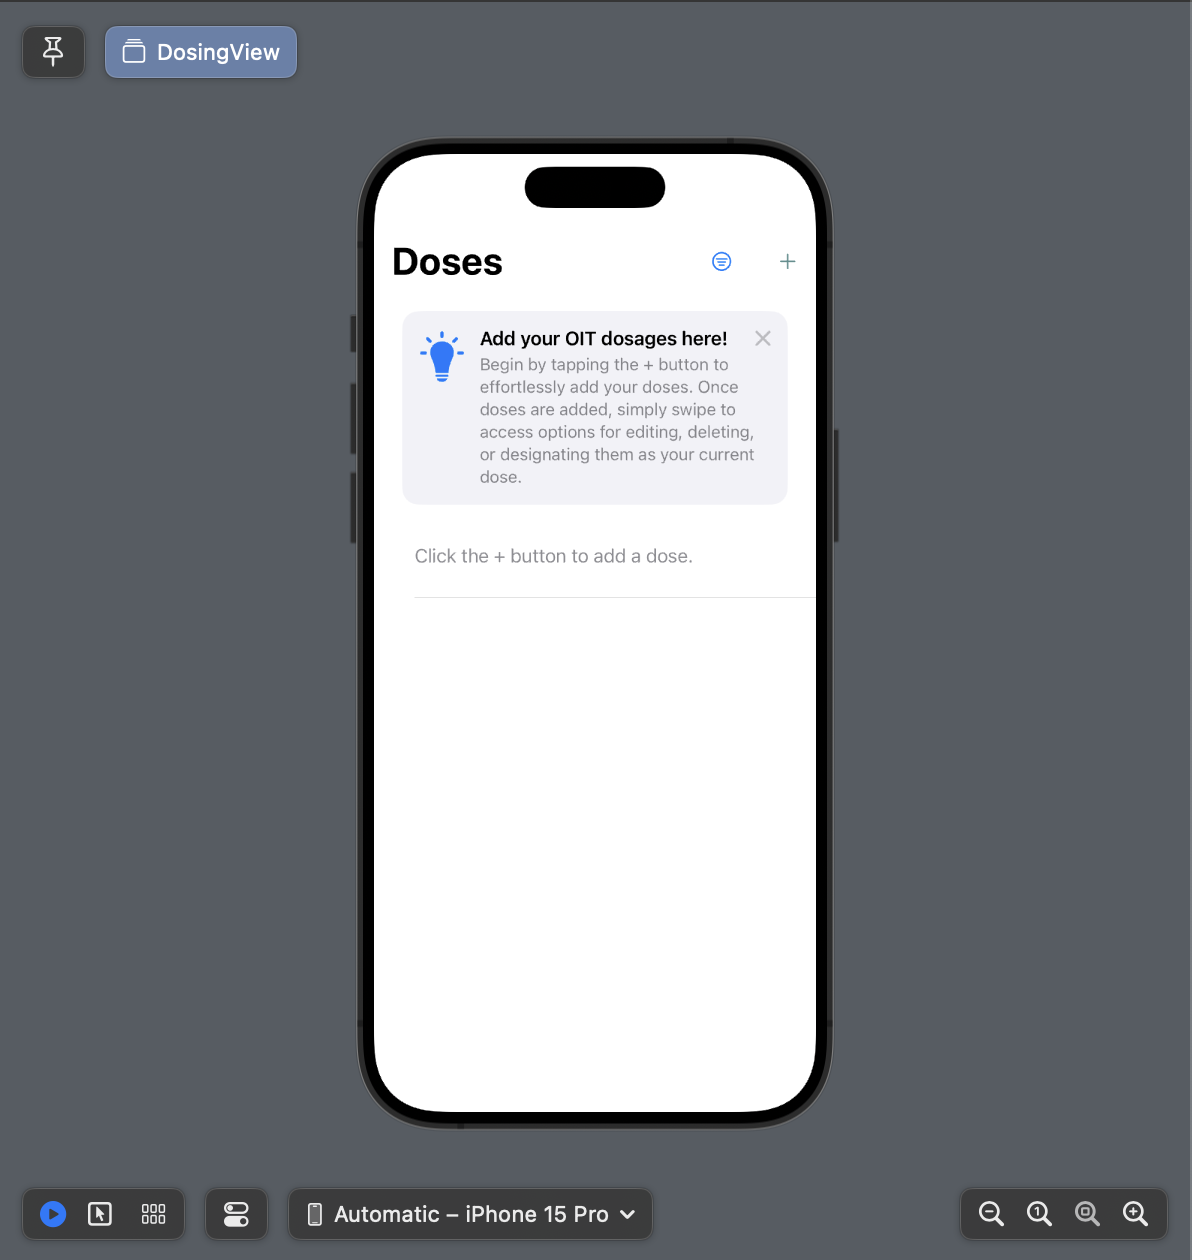
\includegraphics[width=0.5\linewidth]{thesis//chapters//images/SwiftUICanvas.png}
    \caption{SwiftUI Canvas}
    \label{fig:swiftUICanvas}
\end{figure}

\begin{figure} [H]
    \centering
    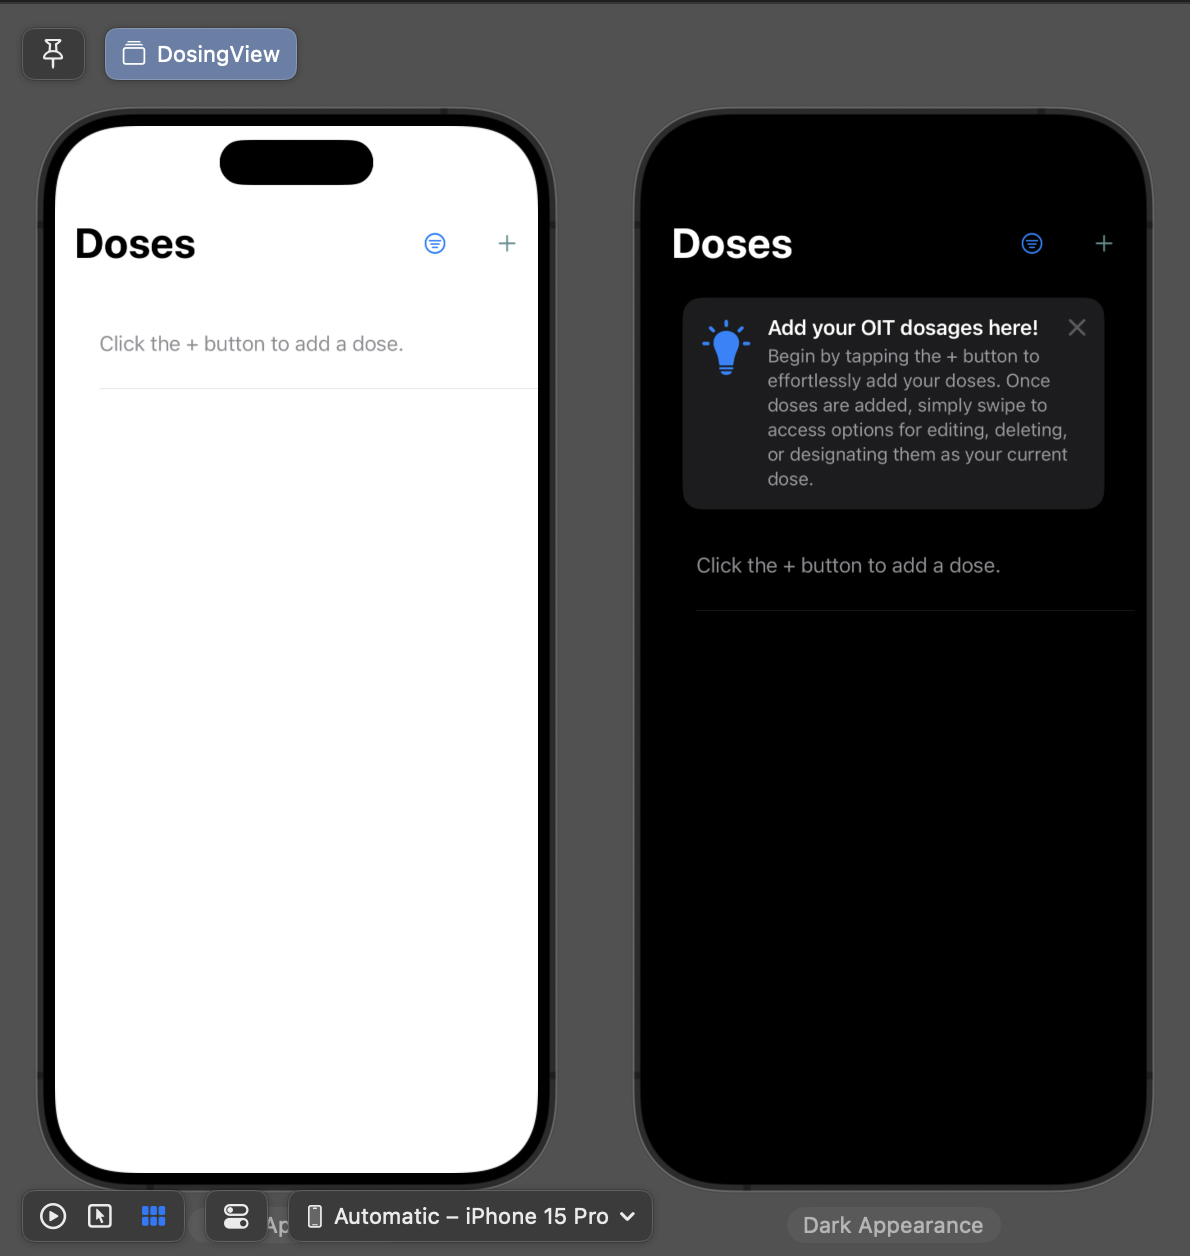
\includegraphics[width=0.5\linewidth]{thesis//chapters//images/SwiftUICanvasColorSchemeVariants.png}
    \caption{Swift UI Canvas Color Scheme Variants}
    \label{fig:swiftUICanvasColorVar}
\end{figure}

\begin{figure} [H]
    \centering
    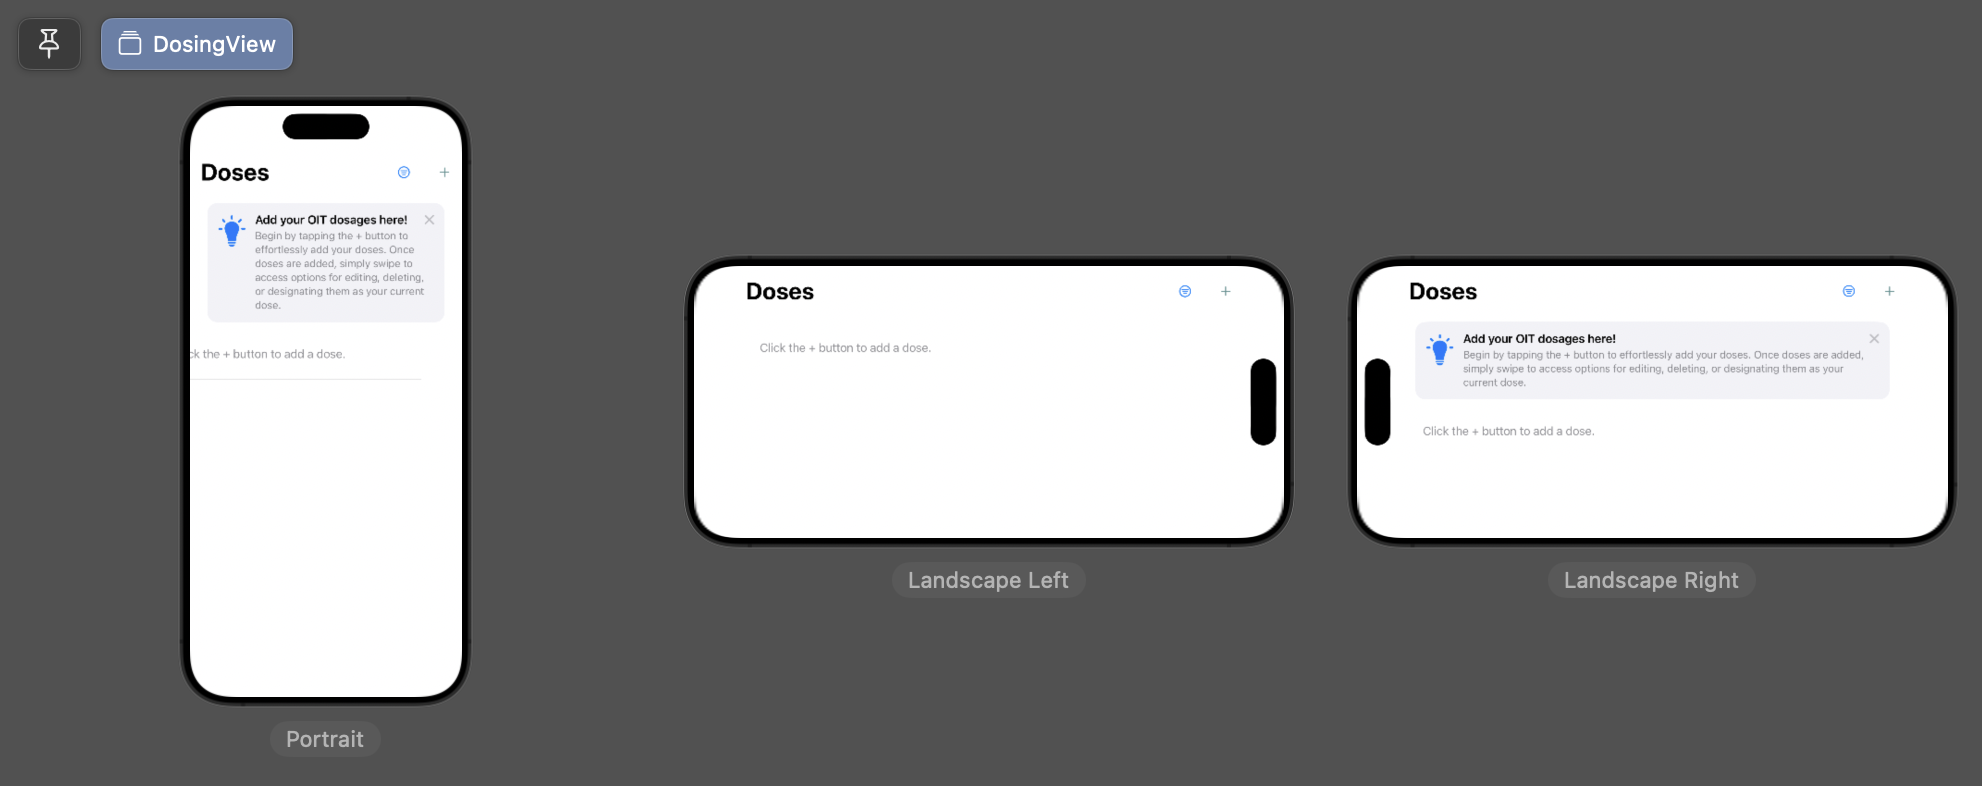
\includegraphics[width=1\linewidth]{thesis//chapters//images/SwiftUICanvasOrientationVariants.png}
    \caption{Swift UI Canvas Orientation Variants}
    \label{fig:swiftUICanvasOrientationVar}
\end{figure}

\begin{figure} [H]
    \centering
    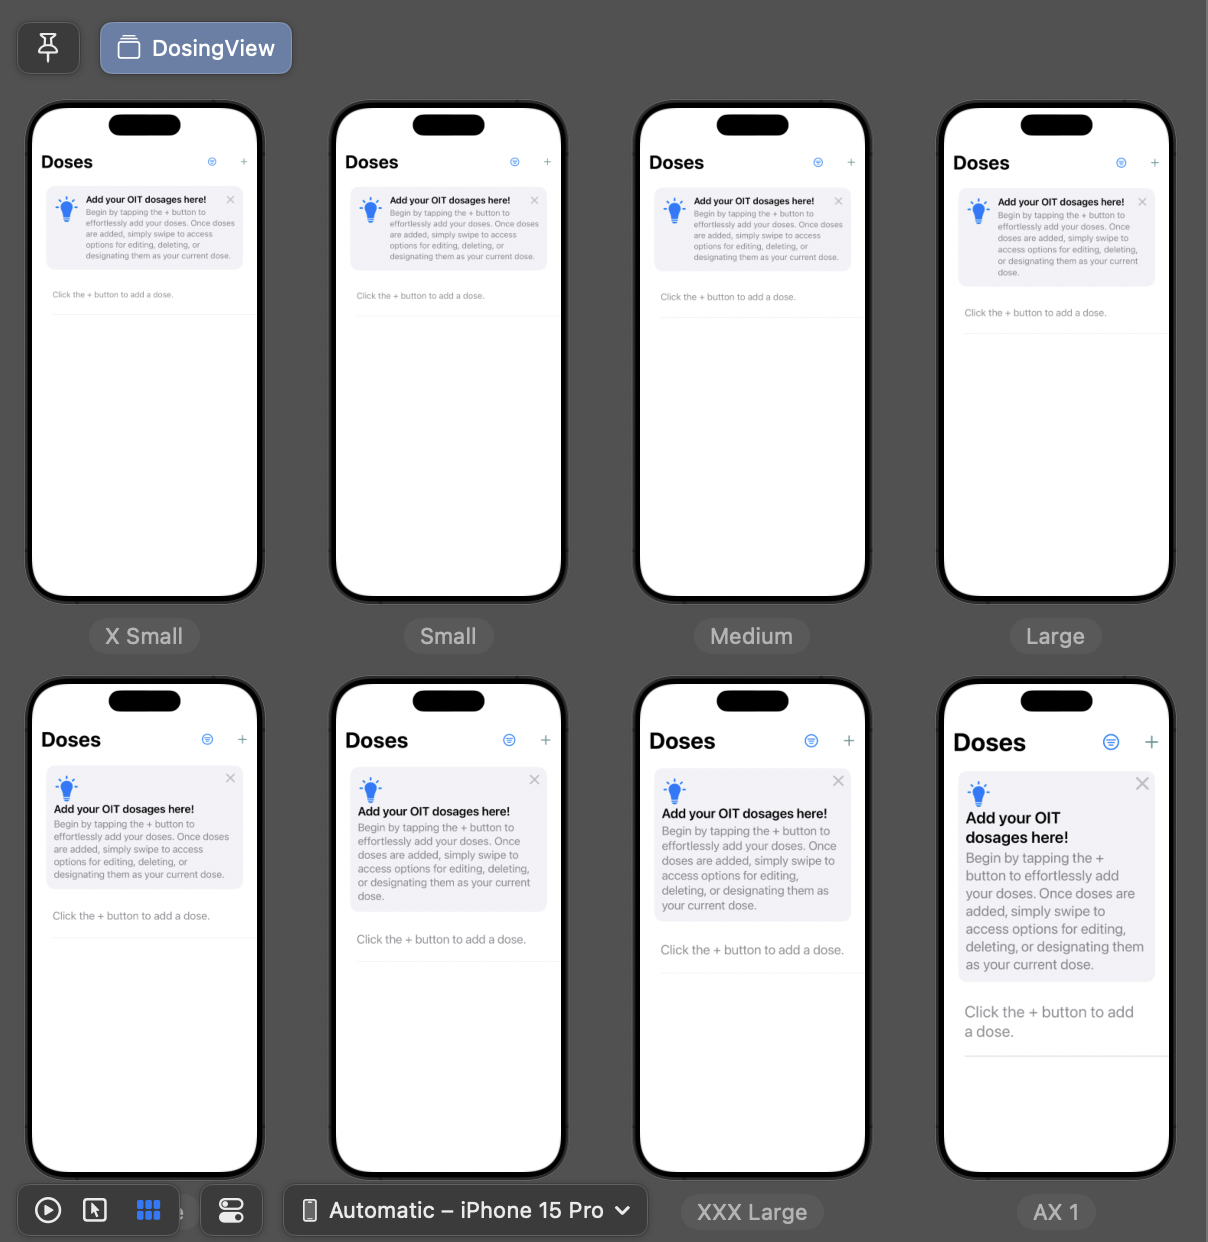
\includegraphics[width=0.75\linewidth]{thesis//chapters//images/SwiftUIDynamicTypeVariants.png}
    \caption{Swift UI Canvas Dynamic Type Variants}
    \label{fig:swiftUICanvasDTVar}
\end{figure}

\begin{figure} [H]
    \centering
    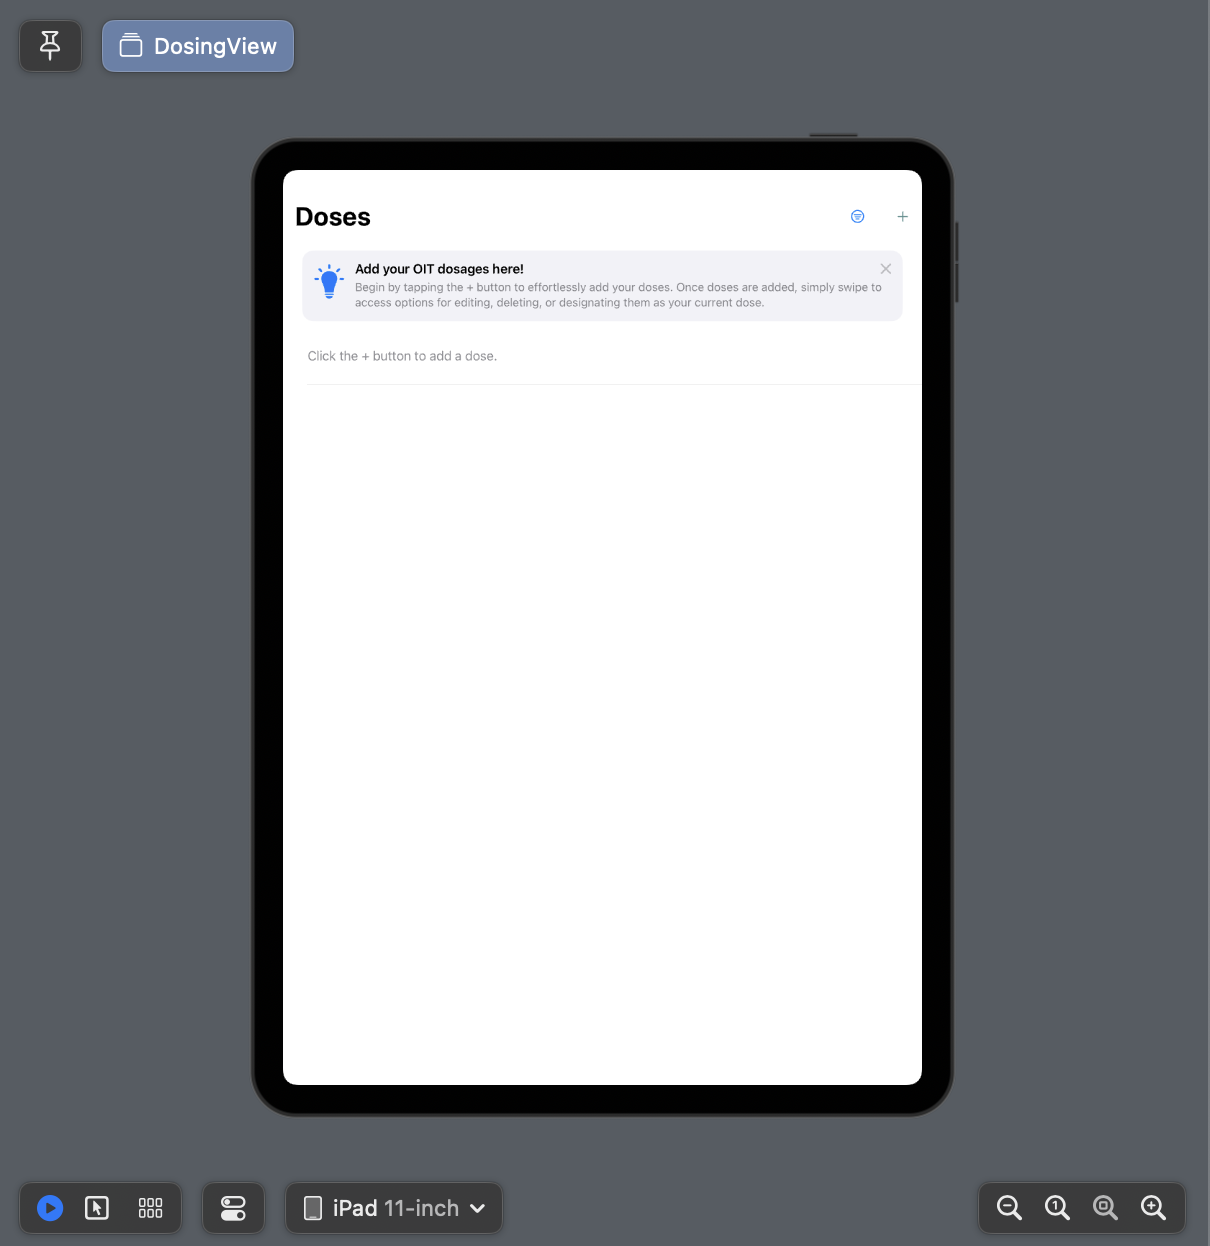
\includegraphics[width=0.75\linewidth]{thesis//chapters//images/SwiftUIDeviceVariant.png}
    \caption{Swift UI Canvas Device Variant}
    \label{fig:deviceVar}
\end{figure}

Additionally, I deployed the application onto my own phone and simulator devices, in order to test the UI in a real world scenario. This was a very helpful way to test the UI and visuals, as certain issues only replicated on device and didn't show up in the Xcode previews.

By conducting comprehensive visual testing, I aimed to guarantee a visually cohesive and appealing user experience.

\section{XCTests and XCUITests}

XCTests and XCUITests served as integral tools for validating the functional aspects of the application throughout its development. These testing frameworks facilitated the creation and execution of unit tests, ensuring the reliability and correctness of the underlying codebase. Regularly running XCTests enabled me to catch and address potential bugs or regressions early in the development process, contributing to the overall stability of the app. Additionally, the use of XCUITests allowed for the automated testing of the app's user interface, simulating user interactions and verifying the correct behavior of UI components.

\section{User Testing}

The user testing phase involved a personalized and hands-on approach to evaluating the application's practical utility.

As a patient undergoing daily maintenance doses of Oral Immunotherapy, I immersed myself in the user experience by utilizing the app in my daily routine. This enabled me to assess the real-world applicability of the application, focusing on aspects such as ease of use, convenience, and the integration of the app into my daily life. Throughout this process, I meticulously logged doses and symptoms, providing valuable insights into the app's functionality and user-friendlines

Although I didn't conduct a formal user study with other users, I did thoroughly design a study below, which could be implemented as a next step.

\subsection{User Study}

To extend the evaluation of the Oral Immunotherapy application beyond individual testing, a formal user study is proposed. The study aims to gather diverse feedback from a representative user population, ensuring a comprehensive understanding of the app's usability, effectiveness, and overall user satisfaction.

\subsubsection{Objectives}

The primary objectives of the user study are as follows:

\begin{itemize}
    \item \textbf{Usability Assessment:} Evaluate the ease of use and user-friendliness of the application, focusing on navigation, feature discoverability, and overall interaction.
    \item \textbf{Effectiveness Evaluation:} Assess the effectiveness of the app in aiding users with daily maintenance doses of Oral Immunotherapy, emphasizing its ability to provide accurate information, timely reminders, and useful insights.
    \item \textbf{Integration into Daily Life: }Examine how well the application integrates into users' daily routines and lifestyles, considering factors such as convenience, time efficiency, and overall impact on their oral immunotherapy management.
    \item \textbf{Feedback Collection:} Gather qualitative and quantitative feedback from participants to identify strengths, weaknesses, and areas for improvement in the application
\end{itemize}

\subsubsection{Participant Recruitment}

Participants for the user study will be recruited from the target user demographic of individuals undergoing oral immunotherapy. Recruitment will aim for diversity in age, technological proficiency, and length of time they have been undergoing oral immunotherapy.

\subsubsection{Methodology}

The user study will adopt a mixed-methods approach, combining quantitative surveys and qualitative interviews to provide a comprehensive assessment.

\begin{itemize}
    \item \textbf{Pre-Study Questionnaire:} Participants will complete a pre-study questionnaire to gather baseline information, including demographics, technological proficiency, and any prior experience with oral immunotherapy management apps.
    \item \textbf{Task-based Testing:} Participants will be given a set of predefined tasks within the application to perform. These tasks will cover essential functionalities, such as setting up their account, logging doses, and accessing relevant information.
    \item \textbf{Post-Task Surveys:} After completing each task, participants will provide feedback through structured surveys, rating their experience based on predefined criteria.
    \item \textbf{Interviews:} A subset of participants will be selected for in-depth interviews to explore their overall impressions, challenges encountered, and suggestions for improvement. These interviews will provide qualitative insights into user experiences and perceptions.
\end{itemize}

\subsubsection{Data Analysis}

Quantitative data from surveys will be analyzed using statistical tools to derive overall performance metrics and identify patterns. Qualitative data from interviews will be analyzed thematically to uncover nuanced feedback and user narratives.

\subsection{Conclusion}

While my personal testing provided valuable insights, the proposed user study is designed to offer a more extensive and diverse evaluation of the Oral Immunotherapy application. Implementing this study as the next step will not only enhance the application's refinement based on collective user feedback but also contribute to its broader acceptance and effectiveness within the target user population.
\chapter{Societal Issues}

When developing a project like this, it is crucial to consider a broad spectrum of societal issues to ensure responsible and ethical innovation. This chapter explores various dimensions, including ethical, social, political, economic, health and safety, manufacturability, sustainability, environmental impact, usability, lifelong learning, and compassion.

\section{Ethical}

Ethical considerations are fundamental to the creation and utilization of any medical application. The oral immunotherapy application adheres to strict ethical standards in terms of user privacy, data security, and informed consent. The collection and handling of user data prioritize confidentiality and comply with relevant data protection regulations. Additionally, the application does not promote any form of discrimination or bias, ensuring fair and equitable access to its benefits. A full, more detailed ethical analysis of the application can be found in Chapter \ref{section:ethics}.

\section{Social}

The social dimension of the oral immunotherapy application focuses on its broader impact on individuals and the community. While the app does not include forums or community features, it still contributes significantly to the social aspect of oral immunotherapy management. By providing a tool for individuals to effectively manage their treatment, the app promotes a sense of autonomy and self-efficacy. This empowerment can lead to improved social interactions and a more active engagement with one's personal health journey. Moreover, the app facilitates better communication between patients and healthcare providers, fostering a collaborative and supportive relationship within the broader healthcare system. The social impact of the application extends beyond user interactions, playing a vital role in enhancing the overall quality of life for individuals undergoing oral immunotherapy.

\section{Political}

Political considerations encompass the alignment of the oral immunotherapy app with healthcare policies and regulations. The application complies with relevant medical standards and guidelines, contributing to the political goal of enhancing patient care and treatment adherence.

\section{Economic}

Economic factors focus on the financial implications of developing and adopting the oral immunotherapy app. The application is designed to be freely accessible to a wide range of users. Additionally, by promoting self-management and reducing healthcare visits, the app has the potential to alleviate economic burdens associated with oral immunotherapy treatments.

\section{Health and Safety}

Health and safety considerations are paramount in the development of a medical application. The app prioritizes user safety by providing accurate information, timely reminders, and emergency protocols. The app encourages responsible self-management while emphasizing the importance of consulting healthcare professionals for critical decisions. Finally, the application complies with Apple Health's constraints and standards, ensuring the data is stored safely and accurately.

\section{Manufacturability}

Manufacturability considerations revolve around the scalability and efficiency of the app's production and distribution. The oral immunotherapy app is designed to be easily scalable, with updates and improvements seamlessly integrated into the user experience. The manufacturing process, in this context, involves software development practices that prioritize reliability, security, and ease of deployment.

\section{Sustainability}

Sustainability considerations encompass the long-term viability and relevance of the oral immunotherapy app. The application is built with a modular and adaptable architecture, allowing for continuous updates and enhancements to meet evolving healthcare needs. Sustainable development practices ensure the app remains effective and relevant in the ever-changing landscape of oral immunotherapy.

\section{Environmental Impact}

The environmental impact of the oral immunotherapy app is predominantly associated with its digital nature, minimizing physical waste and resource consumption. By promoting digital interactions and reducing the need for physical documentation, the app aligns with environmentally conscious practices.

\section{Usability}

Usability is a crucial societal factor that influences the app's acceptance and effectiveness. The oral immunotherapy app prioritizes a user-friendly interface, intuitive navigation, and accessibility features to cater to a diverse user base. Enhancing usability contributes to the app's overall positive societal impact by ensuring broad accessibility and inclusivity.

\section{Lifelong learning}

Lifelong learning considerations emphasize the app's role in providing continuous education and support to users throughout their oral immunotherapy journey. The application incorporates educational resources, updates, and relevant information to foster ongoing learning and empowerment for users, promoting informed decision-making and self-management.

\section{Compassion}

Compassion is woven into the fabric of the oral immunotherapy app, recognizing the challenges individuals face in managing their oral immunotherapy treatments. The app is designed not only to provide practical support but also to empathize with users, acknowledging the emotional and physical aspects of their journey. Through features like personalized reminders and motivational messages, the app aims to instill a sense of compassion and understanding in its interaction with users.
\chapter{An Ethical Analysis}
\label{section:ethics}

Ethical considerations play a crucial role in engineering projects, particularly in the realm of healthcare and medical technology. Engineering endeavors, especially those aimed at improving healthcare outcomes, inherently involve decisions that impact individuals' well-being, safety, and autonomy. Therefore, in this paper, I seek to explore these ethical dimensions within the context of OIT application development, explaining how I designed a solution that not only enhances patient experience and treatment outcomes but also aligns with ethical principles governing healthcare innovation.

The following sections will outline the ethical justification for my project, identify significant ethical issues, provide reasons for decisions and actions, draw on ethical resources, and conclude with reflections on the ethical implications of the project for the broader healthcare landscape. Throughout this paper, I will draw upon established ethical frameworks, engineering codes of ethics, and additional ethical concepts to ensure a comprehensive analysis of the ethical considerations surrounding the development and implementation of the OIT application.

\section{Ethical Justification for the Project}

The very foundation of my project is built upon ethics – particularly the ethical principle of beneficence, which underscores the moral obligation to act for the benefit of others, promoting their well-being and preventing harm. 

As philosopher Immanuel Kant eloquently stated, ``Act in such a way that you treat humanity, whether in your own person or in the person of any other, never merely as a means to an end, but always at the same time as an end'' \cite{Kant}. This principle resonates deeply in the fields of healthcare and technology, where a commitment to improving human welfare should guide innovations. The development of my application embodies this principle by seeking to enhance the lives of individuals undergoing oral immunotherapy. By providing a user-friendly platform for dose tracking, symptom monitoring, and educational resources, my project aims to empower patients to manage their condition and care effectively. In doing so, it not only promotes patients' physical well-being but also acknowledges their autonomy and agency in healthcare decision-making. 

Shifting gears to a utilitarian perspective, it is apparent that my application serves to maximize utility and happiness for the greatest number of people. John Stuart Mill famously posited, ``The creed which accepts as the foundation of morals, Utility, or the Greatest Happiness Principle, holds that actions are right in proportion as they tend to promote happiness, wrong as they tend to produce the reverse of happiness'' \cite{Mill}. From this standpoint, my project is justified by its potential to alleviate suffering and enhance the quality of life for a significant portion of the population affected by food allergies. Furthermore, as outlined in the Introduction, existing systems for logging OIT symptoms and doses rely on cumbersome handwritten logs and papers, causing frustration for both users managing the information and doctors analyzing it. Introducing a centralized digital platform to collect and aggregate this data not only maximizes happiness for patients by simplifying their experience, but also for healthcare providers, streamlining data management and analysis processes.

Drawing inspiration from contemporary philosopher Martha Nussbaum, my project also reflects a commitment to social justice by addressing disparities in healthcare access and information. As Nussbaum asserts, ``Central human capabilities provide the normative focus for political principles and public policy'' \cite{Nussbaum}. By facilitating access to vital resources and information through a mobile application, my project strives to promote equity in healthcare and empower individuals to advocate for their own well-being.

In essence, the ethical justification for my project extends beyond mere technological innovation – it embodies a commitment to compassion, autonomy, and social justice. By drawing upon philosophical insights on beneficence and social justice, my project seeks to contribute meaningfully to the advancement of healthcare and the promotion of human rights.

\section{Identification of Significant Ethical Issues}

The development and implementation of my application necessitate careful consideration of several significant ethical considerations. These encompass privacy and data security, informed consent, equitable access, and the accuracy and reliability of information. Each of these areas presents unique challenges and ethical dilemmas that must be addressed to ensure the ethical integrity of the application and the well-being of its users.

\subsection{Privacy and Data Security}
The issue of privacy and data security within the OIT application is multifaceted and demands careful deliberation. With the collection and storage of sensitive health information, users inherently entrust the application with personal data that can include medical history, allergy profiles, and treatment progress. This data is not only personal but also revealing of vulnerabilities and health conditions. Therefore, the responsibility falls on me, as the developer, to implement stringent security measures to safeguard this information against unauthorized access, breaches, or misuse.

Central to addressing privacy concerns is adherence to regulatory frameworks, such as the Health Insurance Portability and Accountability Act (HIPAA). Compliance with HIPAA standards ensures that patient confidentiality is upheld, and appropriate safeguards are in place to protect health information from unauthorized disclosure. This includes measures such as encryption, access controls, audit trails, and regular security audits to mitigate the risk of data breaches.

Moreover, transparency in data handling practices is paramount to maintaining user trust and confidence in the OIT application. Users should be provided with clear and accessible information about how their data is collected, stored, and used within the application. This includes details on data retention policies and procedures for accessing or deleting personal information. By empowering users with knowledge and control over their data, the application should foster a sense of agency and accountability in its privacy practices.

\subsection{Informed Consent}
Informed consent stands as a cornerstone of ethical practice in healthcare technology, as well as computing in general. The ACM Code of Ethics states, ``Computing professionals should establish transparent policies and procedures that allow individuals to understand what data is being collected and how it is being used, to give informed consent for automatic data collection, and to review, obtain, correct inaccuracies in, and delete their personal data'' \cite{ACM} This principle embodies the principle of respect for individuals' autonomy, acknowledging their right to make informed decisions about their participation in the use of the application and the sharing of their data.

When obtaining informed consent, it is vital that users are provided with comprehensive and comprehensible information about how their data will be collected, stored, and utilized within the application. This includes transparency regarding the purposes for which their data will be used, any potential risks or limitations associated with data sharing, and the mechanisms in place to safeguard their privacy and confidentiality. By arming users with this knowledge, they are better equipped to make informed decisions about their participation in the application and the extent to which they are comfortable sharing their personal information.

Furthermore, obtaining informed consent involves more than just providing information; it also requires ensuring that users have the capacity and opportunity to comprehend and deliberate upon the information presented to them. This is particularly relevant in the context of healthcare technology, where users may vary in their level of health literacy, technological proficiency, and cognitive abilities. As such, efforts should be made to employ clear language, visual aids, and accessible formats to facilitate understanding and decision-making.

Finally, the process of obtaining informed consent should be ongoing and iterative, rather than a one-time event. Users should be allowed to revisit and revise their consent preferences over time, as their circumstances, preferences, and understanding of the application evolve. This dynamic approach to informed consent not only respects users' autonomy but also acknowledges the fluid and evolving nature of their relationship with the application and their personal health information.

\subsection{Equitable Access}
Equitable access to my application is crucial to ensure that individuals of varying ages and technological backgrounds can benefit from its features. Age and digital literacy can significantly impact individuals' ability to access and utilize the application effectively. Given that many oral immunotherapy patients are young, and it's plausible that they, or their parents acting on their behalf, will engage with the application, accommodating varying levels of digital literacy becomes particularly pertinent in my project's design and usability. Another challenge lies in making the application accessible to diverse user groups, including those who may have limited access to technology or face barriers due to socioeconomic factors. 

For older adults or individuals with limited digital literacy, the application should feature intuitive interfaces, clear instructions, and user-friendly design elements to facilitate ease of use. Providing comprehensive user support, such as tutorials or helplines, can further assist users in navigating the application regardless of their technological proficiency. Furthermore, considerations of affordability and cost should be addressed to ensure that my application remains accessible to individuals across socioeconomic backgrounds. Offering the application free of charge can help mitigate financial barriers and ensure equitable access for all.

In summary, ensuring equitable access to my application requires proactive measures to address disparities in digital literacy, socioeconomic status, and more. By prioritizing user accessibility and inclusivity in design and implementation, the application can effectively reach and benefit individuals of diverse backgrounds and circumstances.

\subsection{Accuracy and Reliability of Information}
As mentioned in the Introduction, my application serves as an educational resource for users, providing information about food allergies, oral immunotherapy, and related topics. Ensuring the accuracy and reliability of the information presented is paramount to prevent misinformation and promote informed decision-making among users. Regular updates and validation of content by reputable sources are essential to maintain the integrity of the educational materials.

\section{Ethical Design Rationale}

In light of the significant ethical issues identified in the previous section, I made several decisions regarding the development and features of my application to mitigate ethical quandaries. These decisions were guided by principles of privacy protection, user empowerment, accessibility, and accuracy of information. Below, I elaborate on the rationale behind each decision.

\subsection{Integration with Apple Health and Other Apple Frameworks}

The decision to integrate my app with Apple Health and other Apple frameworks, such as Core Data, demonstrates my commitment to protecting user privacy and ensuring data security within my application. By integrating and aligning with Apple's ecosystem, which is renowned for its stringent privacy policies and robust security measures, my application adopts a proactive approach to safeguarding user data. Apple Health serves as a centralized repository for health-related information, allowing users to securely store and manage their medical data while maintaining control over its access and usage.

One of the key advantages of integrating with Apple Health is the assurance it provides users regarding the confidentiality and integrity of their sensitive health information. Apple has established itself as a trusted steward of user data, implementing encryption, access controls, and other advanced security mechanisms to protect against unauthorized access or breaches. By leveraging Apple's privacy infrastructure, my application can offer users a heightened level of confidence in the protection of their personal health data, fostering trust and credibility in its platform.

Additionally, integration with Core Data enhances the efficiency and reliability of data management within the OIT application. Core Data provides a robust and scalable solution for storing, querying, and manipulating application data, ensuring optimal performance and data integrity. By leveraging Core Data's capabilities, the application can streamline the data storage and retrieval processes while adhering to best practices for data security and privacy.

In essence, the decision to integrate with Apple Health and other Apple frameworks reflects a commitment to prioritizing user privacy and data security within the. By aligning with Apple's ecosystem and leveraging its established privacy infrastructure, the application can offer users a trusted and secure platform for managing their health information.

\subsection{Use of Emojis and Images for Enhanced Understanding}

I decided to incorporate emojis and images throughout my application due to its diverse user base, which has the potential to span across different ages and backgrounds. 

For users who may struggle with textual information due to language barriers, age, or limited literacy skills, emojis and images provide an alternative means of communication that is intuitive and easily understood. Emojis, in particular, convey emotions, actions, and concepts in a concise and visually appealing manner, allowing users to quickly interpret and relate to the content presented. By incorporating emojis strategically throughout the application, the app creates a more inclusive and user-friendly experience, catering to the needs of a diverse audience.

Moreover, the use of images within the application serves to complement textual information, reinforcing key concepts and enhancing comprehension. Visual representations can convey information more effectively than text alone, especially for complex or abstract ideas. By integrating images that illustrate concepts, procedures, or instructions, the application provides users with additional support in understanding and retaining information, regardless of their age or educational background.

\subsection{Inclusion of Tips to Guide Users}

The deliberate inclusion of tips within the OIT application represents a commitment to empowering users and enhancing their experience by offering valuable guidance and support. Recognizing the complexity of the application's features and functionalities, these tips serve as practical suggestions and insights aimed at helping new users navigate and utilize the application effectively.

The application's tips also work to promote informed decision-making and self-management of health among users. By providing users with actionable advice and recommendations, the application equips them with the knowledge and tools needed to make informed choices regarding their health and treatment journey. Whether it's tips on setting up the app, tracking progress, or adhering to treatment protocols, these insights enable users to maximize the benefits derived from the application and optimize their overall health outcomes.

Furthermore, the inclusion of tips reflects a user-centered approach to design and development, placing the needs and preferences of users at the forefront. By anticipating common challenges or questions that users may encounter, the application proactively addresses these concerns through timely and relevant tips. This proactive support not only enhances the user experience but also fosters a sense of confidence and autonomy among users in managing their health.

\subsection{Creation of a User Guide}

The creation of a comprehensive user guide for my application underscores a commitment to transparency, user empowerment, and informed consent. The user guide empowers users with the knowledge and understanding needed to navigate the application effectively. By offering detailed explanations of the application's features and functionalities, users are equipped to make informed choices about how they engage with the application and manage their health data. Moreover, the user guide serves as a reference tool, allowing users to access information about the application's capabilities and privacy practices at their convenience.

And, importantly, the user guide plays a critical role in facilitating informed consent among users. By providing transparency regarding data collection, storage, and utilization practices, the user guide ensures that users are fully aware of how their personal information is being managed within the application. This transparency enables users to make conscious decisions about their participation in the application and the extent to which they are comfortable sharing their data.

\subsection{Making the App Free and Available on the App Store}

The decision to offer my application free of charge and make it readily available on the App Store is driven by a commitment to promoting equitable access and ensuring that individuals from diverse socioeconomic backgrounds can benefit from its features without encountering any cost-related barriers. By offering the application for free, financial constraints are eliminated as a barrier to access, ensuring that individuals of varying economic means can avail themselves of its functionalities. This approach aligns with principles of social justice and inclusivity, ensuring that essential health resources are accessible to all, regardless of their ability to pay.

Additionally, making my application available on the App Store enhances its accessibility and reach, as the platform serves as a central hub for users to discover and download a wide range of applications. By leveraging the widespread availability and convenience of the App Store, the application can reach a broader audience and fulfill its mission of providing valuable health resources to as many individuals as possible.

Offering the application on the App Store also ensures compliance with platform guidelines and standards, further enhancing user trust and credibility. By adhering to App Store regulations, the application demonstrates a commitment to quality, security, and user privacy, thereby instilling confidence in users regarding the integrity and reliability of the platform.

In addition to promoting equitable access for individuals, offering the application free of charge also opens avenues for healthcare providers, including doctors' offices, to distribute the app to their patients. By removing the financial barrier associated with app acquisition, healthcare professionals can readily recommend and provide access to the OIT application as a supplementary tool for patient care.

And, for doctors' offices, the ability to offer the application to patients aligns with a patient-centered approach to healthcare delivery. Healthcare providers can leverage the application as a resource to complement traditional treatment methods, empowering patients to take a more active role in managing their health. By equipping patients with access to the application, doctors' offices can enhance patient education, facilitate treatment adherence, and promote better health outcomes.

Furthermore, the availability of the application free of charge enables doctors' offices to integrate it seamlessly into their existing workflows and patient care protocols. Healthcare professionals can incorporate the application into patient consultations, providing personalized recommendations and guidance tailored to individual treatment plans and goals. This integration fosters a collaborative approach to healthcare, where patients and providers work together towards shared treatment objectives.

As you can see, offering my application for free encourages widespread adoption and utilization among healthcare providers and their patients. By reducing barriers to access, doctors' offices can promote the use of the application as a standard component of care for patients undergoing oral immunotherapy. This widespread adoption not only enhances patient engagement and satisfaction but also facilitates data collection and monitoring, enabling healthcare providers to track patient progress and adjust treatment plans accordingly.

\subsection{Support for Different Font Sizes and Accessibility Features}

Finally, the decision to incorporate support for different font sizes and accessibility features within the application underscores a commitment to promoting inclusivity and ensuring that all users can effectively engage with the application, regardless of their individual accessibility needs.

By offering support for different font sizes, the application acknowledges the diverse range of users who may require adjustments to accommodate visual impairments or preferences. This customization empowers users to personalize their experience with the application, ensuring that they can comfortably read and interact with content without encountering any barriers or difficulties. Whether users require larger font sizes for improved readability or prefer smaller font sizes for increased information density, the application's flexibility ensures that their needs are accommodated.

In addition to supporting different font sizes, the application also incorporates other accessibility features to enhance usability for individuals with diverse needs. By prioritizing accessibility in its design and functionality, the application ensures that all users, regardless of their abilities or limitations, can access its content and features without encountering any accessibility-related barriers.
\chapter{Conclusion}

\section{What I Learned}

\section{Future Applications}
\appendix
\chapter{Code Files}

\section{OITApp.swift}
\lstinputlisting[language=Swift]{thesis/Code/OITApp.swift}

\section{TabbedApplicationView.swift}
\lstinputlisting[language=Swift]{thesis/Code/TabbedApplicationView.swift}

\section{Extensions.swift}
\lstinputlisting[language=Swift]{thesis/Code/Extensions.swift}

\section{AllergenWithDoses.swift}
\lstinputlisting[language=Swift]{thesis/Code/DataModels/AllergenWithDoses.swift}

\section{AntihistamineDose.swift}
\lstinputlisting[language=Swift]{thesis/Code/DataModels/AntihistamineDose.swift}

\section{AntihistamineDoseTransformer.swift}
\lstinputlisting[language=Swift]{thesis/Code/DataModels/AntihistamineDoseTransformer.swift}

\section{Dose.swift}
\lstinputlisting[language=Swift]{thesis/Code/DataModels/Dose.swift}

\section{DoseTransformer.swift}
\lstinputlisting[language=Swift]{thesis/Code/DataModels/DoseTransformer.swift}

\section{DoseViewModel.swift}
\lstinputlisting[language=Swift]{thesis/Code/DataModels/DoseViewModel.swift}

\section{ProfileData}
\lstinputlisting[language=Swift]{thesis/Code/DataModels/ProfileData.swift}

\section{ProfileImageModel.swift}
\lstinputlisting[language=Swift]{thesis/Code/DataModels/ProfileImageModel.swift}

\section{ProfileImageViewModel.swift}
\lstinputlisting[language=Swift]{thesis/Code/DataModels/ProfileImageViewModel.swift}

\section{ProfileViewModel.swift}
\lstinputlisting[language=Swift]{thesis/Code/DataModels/ProfileViewModel.swift}

\section{SelectedAllergensTransformer}
\lstinputlisting[language=Swift]{thesis/Code/DataModels/SelectedAllergensTransformer.swift}

\section{SymptomDataManager.swift}
\lstinputlisting[language=Swift]{thesis/Code/DataModels/SymptomDataManager.swift}

\section{AddDoseView.swift}
\lstinputlisting[language=Swift]{thesis/Code/DosingTab/AddDoseView.swift}

\section{DoseRowView.swift}
\lstinputlisting[language=Swift]{thesis/Code/DosingTab/DoseRowView.swift}

\section{DosingView.swift}
\lstinputlisting[language=Swift]{thesis/Code/DosingTab/DosingView.swift}

\section{DosingViewTip.swift}
\lstinputlisting[language=Swift]{thesis/Code/DosingTab/DosingViewTip.swift}

\section{ArticleRichLink.swift}
\lstinputlisting[language=Swift]{thesis/Code/EducationTab/ArticleRichLink.swift}

\section{ArticleView.swift}
\lstinputlisting[language=Swift]{thesis/Code/EducationTab/ArticleView.swift}

\section{DoctorPhoneTip.swift}
\lstinputlisting[language=Swift]{thesis/Code/EducationTab/DoctorPhoneTip.swift}

\section{EducationView.swift}
\lstinputlisting[language=Swift]{thesis/Code/EducationTab/EducationView.swift}

\section{EducationViewContent.swift}
\lstinputlisting[language=Swift]{thesis/Code/EducationTab/EducationViewContent.swift}

\section{EmergencyServicesTip.swift}
\lstinputlisting[language=Swift]{thesis/Code/EducationTab/EmergencyServicesTip.swift}

\section{ImportantDocumentsTip.swift}
\lstinputlisting[language=Swift]{thesis/Code/EducationTab/ImportantDocumentsTip.swift}

\section{MultiImagePicker.swift}
\lstinputlisting[language=Swift]{thesis/Code/EducationTab/MultiImagePicker.swift}

\section{ResourcesTip.swift}
\lstinputlisting[language=Swift]{thesis/Code/EducationTab/ResourcesTip.swift}

\section{HealthKitManager.swift}
\lstinputlisting[language=Swift]{thesis/Code/HealthKit/HealthKitManager.swift}

\section{HealthKitViewModel.swift}
\lstinputlisting[language=Swift]{thesis/Code/HealthKit/HealthKitViewModel.swift}

\section{AboutYourDoseView.swift}
\lstinputlisting[language=Swift]{thesis/Code/HomeTab/AboutYourDoseView.swift}

\section{CalendarDayView.swift}
\lstinputlisting[language=Swift]{thesis/Code/HomeTab/CalendarDayView.swift}

\section{DosingPopUp.swift}
\lstinputlisting[language=Swift]{thesis/Code/HomeTab/DosingPopUp.swift}

\section{HomeView.swift}
\lstinputlisting[language=Swift]{thesis/Code/HomeTab/HomeView.swift}

\section{ProfileImage.swift}
\lstinputlisting[language=Swift]{thesis/Code/HomeTab/ProfileImage.swift}

\section{SectionHeaderView.swift}
\lstinputlisting[language=Swift]{thesis/Code/HomeTab/SectionHeaderView.swift}

\section{SettingsView.swift}
\lstinputlisting[language=Swift]{thesis/Code/HomeTab/SettingsView.swift}

\section{SymptomsPopUp.swift}
\lstinputlisting[language=Swift]{thesis/Code/HomeTab/SymptomsPopUp.swift}

\section{DosesForMonthView.swift}
\lstinputlisting[language=Swift]{thesis/Code/InsightsTab/DosesForMonthView.swift}

\section{InsightsTip.swift}
\lstinputlisting[language=Swift]{thesis/Code/InsightsTab/InsightsTip.swift}

\section{InsightsView.swift}
\lstinputlisting[language=Swift]{thesis/Code/InsightsTab/InsightsView.swift}

\section{LastReactionInsight.swift}
\lstinputlisting[language=Swift]{thesis/Code/InsightsTab/LastReactionInsight.swift}

\section{Legend.swift}
\lstinputlisting[language=Swift]{thesis/Code/InsightsTab/Legend.swift}

\section{LegendItem.swift}
\lstinputlisting[language=Swift]{thesis/Code/InsightsTab/LegendItem.swift}

\section{SymptomsOverTimeChartView.swift}
\lstinputlisting[language=Swift]{thesis/Code/InsightsTab/SymptomsOverTimeChartView.swift}

\section{SymptomsThisWeekChartView.swift}
\lstinputlisting[language=Swift]{thesis/Code/InsightsTab/SymptomsThisWeekChartView.swift}

\section{GetSetUpView.swift}
\lstinputlisting[language=Swift]{thesis/Code/Onboarding/GetSetUpView.swift}

\section{GetStartedView.swift}
\lstinputlisting[language=Swift]{thesis/Code/Onboarding/GetStartedView.swift}


\begin{thebibliography}{100}
    \bibitem{FARE}Food Allergy Research and Education, “Preventing Food Allergies: Early Interventions | FARE,” \textit{www.foodallergy.org.} https://www.foodallergy.org/research-innovation/accelerating-innovation/early-introduction-and-food-allergy-prevention
    
    \bibitem{Brown} D. Brown et al., “Food allergy-related bullying and associated peer dynamics among black and white children in the forward study,” \textit{Annals of Allergy, Asthma and Immunology, vol. 126, no. 3}, 2021. doi:10.1016/j.anai.2020.10.013
    
    \bibitem{AAAAI} American Academy of Allergy Asthma and Immunology, “The Current State of Oral Immunotherapy (OIT) for the Treatment of Food Allergy,” \textit{Aaaai.org}, 2020. https://www.aaaai.org/Tools-for-the-Public/Conditions-Library/Allergies/The-Current-State-of-Oral-Immunotherapy 

    \bibitem{ACAAI} The American College of Allergy, Asthma and Immunology, “Food Allergy Avoidance,” ACAAI Public Website. https://acaai.org/allergies/management-treatment/living-with-allergies/food-allergy-avoidance/

    \bibitem{Bilucaglia} M. Bilucaglia et al., "Looking through blue glasses: bioelectrical measures to assess the awakening after a calm situation," \textit{2019 41st Annual International Conference of the IEEE Engineering in Medicine and Biology Society (EMBC)}, Berlin, Germany, 2019, pp. 526-529, doi: 10.1109/EMBC.2019.8856486.

    \bibitem{Blumchen} K. Blumchen et al., “Post hoc analysis examining symptom severity reduction and symptom absence during food challenges in individuals who underwent oral immunotherapy for peanut allergy: results from three trials,” Allergy, Asthma, and Clinical Immunology: Official Journal of the Canadian Society of Allergy and Clinical Immunology, vol. 19, no. 1, p. 21, Mar. 2023, doi: https://doi.org/10.1186/s13223-023-00757-8.

    \bibitem{Wanniang} N. Wanniang et al., “Immune signatures predicting the clinical outcome of peanut oral immunotherapy: where we stand,” Frontiers in Allergy, vol. 4, Oct. 2023, doi: https://doi.org/10.3389/falgy.2023.1270344.

    \bibitem{Nairn} S. A. Nairn, “Creating an (ethical) epistemic space for the normalization of clinical and ‘real food’ oral immunotherapy for food allergy,” Health: An Interdisciplinary Journal for the Social Study of Health, Illness and Medicine, p. 136345932211096, Jul. 2022, doi: https://doi.org/10.1177/13634593221109679.

    \bibitem{Dominguez} T. Dominguez, “Food Allergy, Oral Food Challenges, and Oral Immunotherapy,” Physician Assistant Clinics, vol. 8, no. 4, pp. 675–684, Oct. 2023, doi: https://doi.org/10.1016/j.cpha.2023.05.003.

    \bibitem{Gilbert} M. Gilbert T. Chua et al., “Real-world safety and effectiveness analysis of low-dose preschool sesame oral immunotherapy,” Journal of Allergy and Clinical Immunology: Global, vol. 3, no. 1, p. 100171, Feb. 2024, Accessed: Nov. 29, 2023. [Online]. Available: https://doaj.org/article/419f5832508a49019ca3476a94bd4b3d

    \bibitem{Bird} M. D. J. Andrew Bird et al., “Long-term safety and immunologic outcomes of daily oral immunotherapy for peanut allergy,” Journal of Allergy and Clinical Immunology: Global, vol. 2, no. 3, p. 100120, Aug. 2023, Accessed: Nov. 29, 2023. [Online]. Available: https://doaj.org/article/880df47945f042aeb9a2cf79f96c1241

    \bibitem{UML} “About the Unified Modeling Language Specification Version 2.5.1,” www.omg.org. https://www.omg.org/spec/UML/

    \bibitem{IEEEStd} “IEEE Recommended Practice for Software Requirements Specifications,” IEEE Std 830-1998, pp. 1–40, Oct. 1998, doi: https://doi.org/10.1109/IEEESTD.1998.88286.

    \bibitem{ISO} ISO, “ISO/IEC 25010:2011,” ISO, 2011. https://www.iso.org/standard/35733.html 

    \bibitem{HIG} Apple, “Human Interface Guidelines - Design - Apple Developer,” Apple.com, 2019. https://developer.apple.com/design/human-interface-guidelines/

    \bibitem{AppStore} Apple, “App Store Review Guidelines - Apple Developer,” Apple.com, 2019. https://developer.apple.com/app-store/review/guidelines/

    \bibitem{AppleAccessibility} Apple, “Accessibility - Apple Developer,” Apple.com, 2019. https://developer.apple.com/accessibility/

    \bibitem{HIPPA} H. Health, “U.S. Department of Health and Human Services,” HHS.gov, 2019. https://www.hhs.gov

    \bibitem{HealthKit} Apple, “HealthKit | Apple Developer Documentation,” developer.apple.com. https://developer.apple.com/documentation/healthkit

    \bibitem{CareKit} Apple, “CareKit - Apple Developer,” developer.apple.com. https://developer.apple.com/carekit/

    \bibitem{SwiftCharts} [17]Apple, “Apple Developer Documentation,” developer.apple.com. https://developer.apple.com/documentation/charts

    \bibitem{SwiftData} Apple, “SwiftData,” Apple Developer Documentation. https://developer.apple.com/documentation/swiftdata

    \bibitem{Kant} Kant, Immanuel. "Groundwork of the Metaphysics of Morals." Cambridge University Press, 1998.

    \bibitem{Mill} Mill, John Stuart. "Utilitarianism." Edited by George Sher. Hackett Publishing Company, 2001.

    \bibitem{Nussbaum} Nussbaum, Martha C. "Creating Capabilities: The Human Development Approach." Harvard University Press, 2011.

    \bibitem{ACM} ACM Code 2018 Task Force. “ACM Code of Ethics and Professional Conduct.” ACM: Association for Computing Machinery, 2018, https://www.acm.org/code-of-ethics. 

\end{thebibliography}

\backmatter
\end{document}
